% Options for packages loaded elsewhere
\PassOptionsToPackage{unicode}{hyperref}
\PassOptionsToPackage{hyphens}{url}
%
\documentclass[
]{article}
\usepackage{amsmath,amssymb}
\usepackage{lmodern}
\usepackage{iftex}
\ifPDFTeX
  \usepackage[T1]{fontenc}
  \usepackage[utf8]{inputenc}
  \usepackage{textcomp} % provide euro and other symbols
\else % if luatex or xetex
  \usepackage{unicode-math}
  \defaultfontfeatures{Scale=MatchLowercase}
  \defaultfontfeatures[\rmfamily]{Ligatures=TeX,Scale=1}
\fi
% Use upquote if available, for straight quotes in verbatim environments
\IfFileExists{upquote.sty}{\usepackage{upquote}}{}
\IfFileExists{microtype.sty}{% use microtype if available
  \usepackage[]{microtype}
  \UseMicrotypeSet[protrusion]{basicmath} % disable protrusion for tt fonts
}{}
\makeatletter
\@ifundefined{KOMAClassName}{% if non-KOMA class
  \IfFileExists{parskip.sty}{%
    \usepackage{parskip}
  }{% else
    \setlength{\parindent}{0pt}
    \setlength{\parskip}{6pt plus 2pt minus 1pt}}
}{% if KOMA class
  \KOMAoptions{parskip=half}}
\makeatother
\usepackage{xcolor}
\usepackage[margin=1in]{geometry}
\usepackage{color}
\usepackage{fancyvrb}
\newcommand{\VerbBar}{|}
\newcommand{\VERB}{\Verb[commandchars=\\\{\}]}
\DefineVerbatimEnvironment{Highlighting}{Verbatim}{commandchars=\\\{\}}
% Add ',fontsize=\small' for more characters per line
\usepackage{framed}
\definecolor{shadecolor}{RGB}{248,248,248}
\newenvironment{Shaded}{\begin{snugshade}}{\end{snugshade}}
\newcommand{\AlertTok}[1]{\textcolor[rgb]{0.94,0.16,0.16}{#1}}
\newcommand{\AnnotationTok}[1]{\textcolor[rgb]{0.56,0.35,0.01}{\textbf{\textit{#1}}}}
\newcommand{\AttributeTok}[1]{\textcolor[rgb]{0.77,0.63,0.00}{#1}}
\newcommand{\BaseNTok}[1]{\textcolor[rgb]{0.00,0.00,0.81}{#1}}
\newcommand{\BuiltInTok}[1]{#1}
\newcommand{\CharTok}[1]{\textcolor[rgb]{0.31,0.60,0.02}{#1}}
\newcommand{\CommentTok}[1]{\textcolor[rgb]{0.56,0.35,0.01}{\textit{#1}}}
\newcommand{\CommentVarTok}[1]{\textcolor[rgb]{0.56,0.35,0.01}{\textbf{\textit{#1}}}}
\newcommand{\ConstantTok}[1]{\textcolor[rgb]{0.00,0.00,0.00}{#1}}
\newcommand{\ControlFlowTok}[1]{\textcolor[rgb]{0.13,0.29,0.53}{\textbf{#1}}}
\newcommand{\DataTypeTok}[1]{\textcolor[rgb]{0.13,0.29,0.53}{#1}}
\newcommand{\DecValTok}[1]{\textcolor[rgb]{0.00,0.00,0.81}{#1}}
\newcommand{\DocumentationTok}[1]{\textcolor[rgb]{0.56,0.35,0.01}{\textbf{\textit{#1}}}}
\newcommand{\ErrorTok}[1]{\textcolor[rgb]{0.64,0.00,0.00}{\textbf{#1}}}
\newcommand{\ExtensionTok}[1]{#1}
\newcommand{\FloatTok}[1]{\textcolor[rgb]{0.00,0.00,0.81}{#1}}
\newcommand{\FunctionTok}[1]{\textcolor[rgb]{0.00,0.00,0.00}{#1}}
\newcommand{\ImportTok}[1]{#1}
\newcommand{\InformationTok}[1]{\textcolor[rgb]{0.56,0.35,0.01}{\textbf{\textit{#1}}}}
\newcommand{\KeywordTok}[1]{\textcolor[rgb]{0.13,0.29,0.53}{\textbf{#1}}}
\newcommand{\NormalTok}[1]{#1}
\newcommand{\OperatorTok}[1]{\textcolor[rgb]{0.81,0.36,0.00}{\textbf{#1}}}
\newcommand{\OtherTok}[1]{\textcolor[rgb]{0.56,0.35,0.01}{#1}}
\newcommand{\PreprocessorTok}[1]{\textcolor[rgb]{0.56,0.35,0.01}{\textit{#1}}}
\newcommand{\RegionMarkerTok}[1]{#1}
\newcommand{\SpecialCharTok}[1]{\textcolor[rgb]{0.00,0.00,0.00}{#1}}
\newcommand{\SpecialStringTok}[1]{\textcolor[rgb]{0.31,0.60,0.02}{#1}}
\newcommand{\StringTok}[1]{\textcolor[rgb]{0.31,0.60,0.02}{#1}}
\newcommand{\VariableTok}[1]{\textcolor[rgb]{0.00,0.00,0.00}{#1}}
\newcommand{\VerbatimStringTok}[1]{\textcolor[rgb]{0.31,0.60,0.02}{#1}}
\newcommand{\WarningTok}[1]{\textcolor[rgb]{0.56,0.35,0.01}{\textbf{\textit{#1}}}}
\usepackage{longtable,booktabs,array}
\usepackage{calc} % for calculating minipage widths
% Correct order of tables after \paragraph or \subparagraph
\usepackage{etoolbox}
\makeatletter
\patchcmd\longtable{\par}{\if@noskipsec\mbox{}\fi\par}{}{}
\makeatother
% Allow footnotes in longtable head/foot
\IfFileExists{footnotehyper.sty}{\usepackage{footnotehyper}}{\usepackage{footnote}}
\makesavenoteenv{longtable}
\usepackage{graphicx}
\makeatletter
\def\maxwidth{\ifdim\Gin@nat@width>\linewidth\linewidth\else\Gin@nat@width\fi}
\def\maxheight{\ifdim\Gin@nat@height>\textheight\textheight\else\Gin@nat@height\fi}
\makeatother
% Scale images if necessary, so that they will not overflow the page
% margins by default, and it is still possible to overwrite the defaults
% using explicit options in \includegraphics[width, height, ...]{}
\setkeys{Gin}{width=\maxwidth,height=\maxheight,keepaspectratio}
% Set default figure placement to htbp
\makeatletter
\def\fps@figure{htbp}
\makeatother
\setlength{\emergencystretch}{3em} % prevent overfull lines
\providecommand{\tightlist}{%
  \setlength{\itemsep}{0pt}\setlength{\parskip}{0pt}}
\setcounter{secnumdepth}{-\maxdimen} % remove section numbering
\usepackage{fontspec}
\usepackage{tikz}
\usepackage{ctable}
\usepackage{url}
\ifLuaTeX
  \usepackage{selnolig}  % disable illegal ligatures
\fi
\IfFileExists{bookmark.sty}{\usepackage{bookmark}}{\usepackage{hyperref}}
\IfFileExists{xurl.sty}{\usepackage{xurl}}{} % add URL line breaks if available
\urlstyle{same} % disable monospaced font for URLs
\hypersetup{
  pdftitle={MATHS 7107 Data Taming Assignment Final Report},
  pdfauthor={Chang Dong},
  hidelinks,
  pdfcreator={LaTeX via pandoc}}

\title{MATHS 7107 Data Taming Assignment Final Report}
\author{Chang Dong}
\date{2023-04-24}

\begin{document}
\maketitle

\hypertarget{appendix}{%
\section{Appendix}\label{appendix}}

\begin{Shaded}
\begin{Highlighting}[]
\NormalTok{pacman}\SpecialCharTok{::}\FunctionTok{p\_load}\NormalTok{(skimr, tidyverse, tidymodels, themis, recipes, dials,kknn, vip,forcats,caret,MASS,discrim,yardstick,pROC)}
\end{Highlighting}
\end{Shaded}

\hypertarget{data-import}{%
\subsection{1.1 Data import}\label{data-import}}

\begin{Shaded}
\begin{Highlighting}[]
\NormalTok{spotify\_songs\_origin }\OtherTok{\textless{}{-}}\NormalTok{ readr}\SpecialCharTok{::}\FunctionTok{read\_csv}\NormalTok{(}\StringTok{\textquotesingle{}https://raw.githubusercontent.com/rfordatascience/tidytuesday/master/data/2020/2020{-}01{-}21/spotify\_songs.csv\textquotesingle{}}\NormalTok{)}
\end{Highlighting}
\end{Shaded}

\begin{verbatim}
## Rows: 32833 Columns: 23
## -- Column specification --------------------------------------------------------
## Delimiter: ","
## chr (10): track_id, track_name, track_artist, track_album_id, track_album_na...
## dbl (13): track_popularity, danceability, energy, key, loudness, mode, speec...
## 
## i Use `spec()` to retrieve the full column specification for this data.
## i Specify the column types or set `show_col_types = FALSE` to quiet this message.
\end{verbatim}

\begin{Shaded}
\begin{Highlighting}[]
\FunctionTok{skim}\NormalTok{(spotify\_songs\_origin)}
\end{Highlighting}
\end{Shaded}

\begin{longtable}[]{@{}ll@{}}
\caption{Data summary}\tabularnewline
\toprule()
\endhead
Name & spotify\_songs\_origin \\
Number of rows & 32833 \\
Number of columns & 23 \\
\_\_\_\_\_\_\_\_\_\_\_\_\_\_\_\_\_\_\_\_\_\_\_ & \\
Column type frequency: & \\
character & 10 \\
numeric & 13 \\
\_\_\_\_\_\_\_\_\_\_\_\_\_\_\_\_\_\_\_\_\_\_\_\_ & \\
Group variables & None \\
\bottomrule()
\end{longtable}

\textbf{Variable type: character}

\begin{longtable}[]{@{}
  >{\raggedright\arraybackslash}p{(\columnwidth - 14\tabcolsep) * \real{0.3012}}
  >{\raggedleft\arraybackslash}p{(\columnwidth - 14\tabcolsep) * \real{0.1205}}
  >{\raggedleft\arraybackslash}p{(\columnwidth - 14\tabcolsep) * \real{0.1687}}
  >{\raggedleft\arraybackslash}p{(\columnwidth - 14\tabcolsep) * \real{0.0482}}
  >{\raggedleft\arraybackslash}p{(\columnwidth - 14\tabcolsep) * \real{0.0482}}
  >{\raggedleft\arraybackslash}p{(\columnwidth - 14\tabcolsep) * \real{0.0723}}
  >{\raggedleft\arraybackslash}p{(\columnwidth - 14\tabcolsep) * \real{0.1084}}
  >{\raggedleft\arraybackslash}p{(\columnwidth - 14\tabcolsep) * \real{0.1325}}@{}}
\toprule()
\begin{minipage}[b]{\linewidth}\raggedright
skim\_variable
\end{minipage} & \begin{minipage}[b]{\linewidth}\raggedleft
n\_missing
\end{minipage} & \begin{minipage}[b]{\linewidth}\raggedleft
complete\_rate
\end{minipage} & \begin{minipage}[b]{\linewidth}\raggedleft
min
\end{minipage} & \begin{minipage}[b]{\linewidth}\raggedleft
max
\end{minipage} & \begin{minipage}[b]{\linewidth}\raggedleft
empty
\end{minipage} & \begin{minipage}[b]{\linewidth}\raggedleft
n\_unique
\end{minipage} & \begin{minipage}[b]{\linewidth}\raggedleft
whitespace
\end{minipage} \\
\midrule()
\endhead
track\_id & 0 & 1 & 22 & 22 & 0 & 28356 & 0 \\
track\_name & 5 & 1 & 1 & 144 & 0 & 23449 & 0 \\
track\_artist & 5 & 1 & 2 & 69 & 0 & 10692 & 0 \\
track\_album\_id & 0 & 1 & 22 & 22 & 0 & 22545 & 0 \\
track\_album\_name & 5 & 1 & 1 & 151 & 0 & 19743 & 0 \\
track\_album\_release\_date & 0 & 1 & 4 & 10 & 0 & 4530 & 0 \\
playlist\_name & 0 & 1 & 6 & 120 & 0 & 449 & 0 \\
playlist\_id & 0 & 1 & 22 & 22 & 0 & 471 & 0 \\
playlist\_genre & 0 & 1 & 3 & 5 & 0 & 6 & 0 \\
playlist\_subgenre & 0 & 1 & 4 & 25 & 0 & 24 & 0 \\
\bottomrule()
\end{longtable}

\textbf{Variable type: numeric}

\begin{longtable}[]{@{}
  >{\raggedright\arraybackslash}p{(\columnwidth - 20\tabcolsep) * \real{0.1491}}
  >{\raggedleft\arraybackslash}p{(\columnwidth - 20\tabcolsep) * \real{0.0877}}
  >{\raggedleft\arraybackslash}p{(\columnwidth - 20\tabcolsep) * \real{0.1228}}
  >{\raggedleft\arraybackslash}p{(\columnwidth - 20\tabcolsep) * \real{0.0877}}
  >{\raggedleft\arraybackslash}p{(\columnwidth - 20\tabcolsep) * \real{0.0789}}
  >{\raggedleft\arraybackslash}p{(\columnwidth - 20\tabcolsep) * \real{0.0702}}
  >{\raggedleft\arraybackslash}p{(\columnwidth - 20\tabcolsep) * \real{0.0877}}
  >{\raggedleft\arraybackslash}p{(\columnwidth - 20\tabcolsep) * \real{0.0877}}
  >{\raggedleft\arraybackslash}p{(\columnwidth - 20\tabcolsep) * \real{0.0877}}
  >{\raggedleft\arraybackslash}p{(\columnwidth - 20\tabcolsep) * \real{0.0877}}
  >{\raggedright\arraybackslash}p{(\columnwidth - 20\tabcolsep) * \real{0.0526}}@{}}
\toprule()
\begin{minipage}[b]{\linewidth}\raggedright
skim\_variable
\end{minipage} & \begin{minipage}[b]{\linewidth}\raggedleft
n\_missing
\end{minipage} & \begin{minipage}[b]{\linewidth}\raggedleft
complete\_rate
\end{minipage} & \begin{minipage}[b]{\linewidth}\raggedleft
mean
\end{minipage} & \begin{minipage}[b]{\linewidth}\raggedleft
sd
\end{minipage} & \begin{minipage}[b]{\linewidth}\raggedleft
p0
\end{minipage} & \begin{minipage}[b]{\linewidth}\raggedleft
p25
\end{minipage} & \begin{minipage}[b]{\linewidth}\raggedleft
p50
\end{minipage} & \begin{minipage}[b]{\linewidth}\raggedleft
p75
\end{minipage} & \begin{minipage}[b]{\linewidth}\raggedleft
p100
\end{minipage} & \begin{minipage}[b]{\linewidth}\raggedright
hist
\end{minipage} \\
\midrule()
\endhead
track\_popularity & 0 & 1 & 42.48 & 24.98 & 0.00 & 24.00 & 45.00 & 62.00
& 100.00 & ▆▆▇▆▁ \\
danceability & 0 & 1 & 0.65 & 0.15 & 0.00 & 0.56 & 0.67 & 0.76 & 0.98 &
▁▁▃▇▃ \\
energy & 0 & 1 & 0.70 & 0.18 & 0.00 & 0.58 & 0.72 & 0.84 & 1.00 &
▁▁▅▇▇ \\
key & 0 & 1 & 5.37 & 3.61 & 0.00 & 2.00 & 6.00 & 9.00 & 11.00 & ▇▂▅▅▆ \\
loudness & 0 & 1 & -6.72 & 2.99 & -46.45 & -8.17 & -6.17 & -4.64 & 1.27
& ▁▁▁▂▇ \\
mode & 0 & 1 & 0.57 & 0.50 & 0.00 & 0.00 & 1.00 & 1.00 & 1.00 & ▆▁▁▁▇ \\
speechiness & 0 & 1 & 0.11 & 0.10 & 0.00 & 0.04 & 0.06 & 0.13 & 0.92 &
▇▂▁▁▁ \\
acousticness & 0 & 1 & 0.18 & 0.22 & 0.00 & 0.02 & 0.08 & 0.26 & 0.99 &
▇▂▁▁▁ \\
instrumentalness & 0 & 1 & 0.08 & 0.22 & 0.00 & 0.00 & 0.00 & 0.00 &
0.99 & ▇▁▁▁▁ \\
liveness & 0 & 1 & 0.19 & 0.15 & 0.00 & 0.09 & 0.13 & 0.25 & 1.00 &
▇▃▁▁▁ \\
valence & 0 & 1 & 0.51 & 0.23 & 0.00 & 0.33 & 0.51 & 0.69 & 0.99 &
▃▇▇▇▃ \\
tempo & 0 & 1 & 120.88 & 26.90 & 0.00 & 99.96 & 121.98 & 133.92 & 239.44
& ▁▂▇▂▁ \\
duration\_ms & 0 & 1 & 225799.81 & 59834.01 & 4000.00 & 187819.00 &
216000.00 & 253585.00 & 517810.00 & ▁▇▇▁▁ \\
\bottomrule()
\end{longtable}

\hypertarget{data-cleanning-method}{%
\subsection{1.2 Data Cleanning Method}\label{data-cleanning-method}}

These have n\_unique more than 1000 should be considered as Text instead
of Categorical data (``track\_id'',``track\_name'', ``track\_artist'',
``track\_album\_id'', ``track\_album\_name''), ,
``track\_album\_release\_date'' is not included, because we know it is a
time series should be numerical.

\begin{Shaded}
\begin{Highlighting}[]
\NormalTok{text\_variables }\OtherTok{\textless{}{-}} \FunctionTok{c}\NormalTok{(}\StringTok{"track\_id"}\NormalTok{, }\StringTok{"track\_name"}\NormalTok{, }\StringTok{"track\_artist"}\NormalTok{, }\StringTok{"track\_album\_id"}\NormalTok{, }\StringTok{"track\_album\_name"}\NormalTok{)}

\NormalTok{spotify\_songs }\OtherTok{\textless{}{-}}\NormalTok{ spotify\_songs\_origin }\SpecialCharTok{\%\textgreater{}\%}
\NormalTok{  dplyr}\SpecialCharTok{::}\FunctionTok{select}\NormalTok{(}\SpecialCharTok{{-}}\NormalTok{dplyr}\SpecialCharTok{::}\FunctionTok{any\_of}\NormalTok{(text\_variables))}
\end{Highlighting}
\end{Shaded}

Categorical Data (factor)

\begin{Shaded}
\begin{Highlighting}[]
\NormalTok{categorical\_variables }\OtherTok{\textless{}{-}} \FunctionTok{c}\NormalTok{(}\StringTok{"playlist\_name"}\NormalTok{, }\StringTok{"playlist\_id"}\NormalTok{, }\StringTok{"playlist\_genre"}\NormalTok{, }\StringTok{"playlist\_subgenre"}\NormalTok{)}

\NormalTok{spotify\_songs }\OtherTok{\textless{}{-}}\NormalTok{ spotify\_songs }\SpecialCharTok{\%\textgreater{}\%}
  \FunctionTok{mutate}\NormalTok{(}\FunctionTok{across}\NormalTok{(}\FunctionTok{all\_of}\NormalTok{(categorical\_variables), as.factor)) }
\end{Highlighting}
\end{Shaded}

Numerical Data (numerical)

\begin{Shaded}
\begin{Highlighting}[]
\NormalTok{numerical\_variables }\OtherTok{\textless{}{-}} \FunctionTok{c}\NormalTok{(}\StringTok{"track\_popularity"}\NormalTok{,}\StringTok{"danceability"}\NormalTok{, }\StringTok{"energy"}\NormalTok{, }\StringTok{"key"}\NormalTok{, }
                           \StringTok{"loudness"}\NormalTok{,}\StringTok{"mode"}\NormalTok{, }\StringTok{"speechiness"}\NormalTok{,}\StringTok{"acousticness"}\NormalTok{,}
                           \StringTok{"instrumentalness"}\NormalTok{, }\StringTok{"liveness"}\NormalTok{, }\StringTok{"valence"}\NormalTok{, }
                           \StringTok{"tempo"}\NormalTok{, }\StringTok{"duration\_ms"}\NormalTok{)             }

\NormalTok{spotify\_songs }\OtherTok{\textless{}{-}}\NormalTok{ spotify\_songs }\SpecialCharTok{\%\textgreater{}\%}
  \FunctionTok{mutate}\NormalTok{(}\FunctionTok{across}\NormalTok{(}\FunctionTok{all\_of}\NormalTok{(numerical\_variables), as.numeric))}

\NormalTok{spotify\_songs }\OtherTok{\textless{}{-}}\NormalTok{ spotify\_songs }\SpecialCharTok{\%\textgreater{}\%}
  \FunctionTok{mutate}\NormalTok{(}\AttributeTok{track\_album\_release\_year =} \FunctionTok{as.numeric}\NormalTok{(}\FunctionTok{format}\NormalTok{(}\FunctionTok{as.Date}\NormalTok{(track\_album\_release\_date, }\AttributeTok{format =} \StringTok{"\%Y{-}\%m{-}\%d"}\NormalTok{), }\StringTok{"\%Y"}\NormalTok{))) }\SpecialCharTok{\%\textgreater{}\%}
\NormalTok{  dplyr}\SpecialCharTok{::}\FunctionTok{select}\NormalTok{(}\SpecialCharTok{{-}}\NormalTok{track\_album\_release\_date)}

\NormalTok{numerical\_variables }\OtherTok{\textless{}{-}} \FunctionTok{c}\NormalTok{(numerical\_variables, }\StringTok{"track\_album\_release\_year"}\NormalTok{)}
\end{Highlighting}
\end{Shaded}

\begin{Shaded}
\begin{Highlighting}[]
\FunctionTok{skim}\NormalTok{(spotify\_songs)}
\end{Highlighting}
\end{Shaded}

\begin{longtable}[]{@{}ll@{}}
\caption{Data summary}\tabularnewline
\toprule()
\endhead
Name & spotify\_songs \\
Number of rows & 32833 \\
Number of columns & 18 \\
\_\_\_\_\_\_\_\_\_\_\_\_\_\_\_\_\_\_\_\_\_\_\_ & \\
Column type frequency: & \\
factor & 4 \\
numeric & 14 \\
\_\_\_\_\_\_\_\_\_\_\_\_\_\_\_\_\_\_\_\_\_\_\_\_ & \\
Group variables & None \\
\bottomrule()
\end{longtable}

\textbf{Variable type: factor}

\begin{longtable}[]{@{}
  >{\raggedright\arraybackslash}p{(\columnwidth - 10\tabcolsep) * \real{0.1765}}
  >{\raggedleft\arraybackslash}p{(\columnwidth - 10\tabcolsep) * \real{0.0980}}
  >{\raggedleft\arraybackslash}p{(\columnwidth - 10\tabcolsep) * \real{0.1373}}
  >{\raggedright\arraybackslash}p{(\columnwidth - 10\tabcolsep) * \real{0.0784}}
  >{\raggedleft\arraybackslash}p{(\columnwidth - 10\tabcolsep) * \real{0.0882}}
  >{\raggedright\arraybackslash}p{(\columnwidth - 10\tabcolsep) * \real{0.4216}}@{}}
\toprule()
\begin{minipage}[b]{\linewidth}\raggedright
skim\_variable
\end{minipage} & \begin{minipage}[b]{\linewidth}\raggedleft
n\_missing
\end{minipage} & \begin{minipage}[b]{\linewidth}\raggedleft
complete\_rate
\end{minipage} & \begin{minipage}[b]{\linewidth}\raggedright
ordered
\end{minipage} & \begin{minipage}[b]{\linewidth}\raggedleft
n\_unique
\end{minipage} & \begin{minipage}[b]{\linewidth}\raggedright
top\_counts
\end{minipage} \\
\midrule()
\endhead
playlist\_name & 0 & 1 & FALSE & 449 & Ind: 308, 202: 247, Per: 244,
Har: 219 \\
playlist\_id & 0 & 1 & FALSE & 471 & 4Jk: 247, 37i: 198, 6Kn: 195, 3xM:
189 \\
playlist\_genre & 0 & 1 & FALSE & 6 & edm: 6043, rap: 5746, pop: 5507,
r\&b: 5431 \\
playlist\_subgenre & 0 & 1 & FALSE & 24 & pro: 1809, sou: 1675, ind:
1672, lat: 1656 \\
\bottomrule()
\end{longtable}

\textbf{Variable type: numeric}

\begin{longtable}[]{@{}
  >{\raggedright\arraybackslash}p{(\columnwidth - 20\tabcolsep) * \real{0.2049}}
  >{\raggedleft\arraybackslash}p{(\columnwidth - 20\tabcolsep) * \real{0.0820}}
  >{\raggedleft\arraybackslash}p{(\columnwidth - 20\tabcolsep) * \real{0.1148}}
  >{\raggedleft\arraybackslash}p{(\columnwidth - 20\tabcolsep) * \real{0.0820}}
  >{\raggedleft\arraybackslash}p{(\columnwidth - 20\tabcolsep) * \real{0.0738}}
  >{\raggedleft\arraybackslash}p{(\columnwidth - 20\tabcolsep) * \real{0.0656}}
  >{\raggedleft\arraybackslash}p{(\columnwidth - 20\tabcolsep) * \real{0.0820}}
  >{\raggedleft\arraybackslash}p{(\columnwidth - 20\tabcolsep) * \real{0.0820}}
  >{\raggedleft\arraybackslash}p{(\columnwidth - 20\tabcolsep) * \real{0.0820}}
  >{\raggedleft\arraybackslash}p{(\columnwidth - 20\tabcolsep) * \real{0.0820}}
  >{\raggedright\arraybackslash}p{(\columnwidth - 20\tabcolsep) * \real{0.0492}}@{}}
\toprule()
\begin{minipage}[b]{\linewidth}\raggedright
skim\_variable
\end{minipage} & \begin{minipage}[b]{\linewidth}\raggedleft
n\_missing
\end{minipage} & \begin{minipage}[b]{\linewidth}\raggedleft
complete\_rate
\end{minipage} & \begin{minipage}[b]{\linewidth}\raggedleft
mean
\end{minipage} & \begin{minipage}[b]{\linewidth}\raggedleft
sd
\end{minipage} & \begin{minipage}[b]{\linewidth}\raggedleft
p0
\end{minipage} & \begin{minipage}[b]{\linewidth}\raggedleft
p25
\end{minipage} & \begin{minipage}[b]{\linewidth}\raggedleft
p50
\end{minipage} & \begin{minipage}[b]{\linewidth}\raggedleft
p75
\end{minipage} & \begin{minipage}[b]{\linewidth}\raggedleft
p100
\end{minipage} & \begin{minipage}[b]{\linewidth}\raggedright
hist
\end{minipage} \\
\midrule()
\endhead
track\_popularity & 0 & 1.00 & 42.48 & 24.98 & 0.00 & 24.00 & 45.00 &
62.00 & 100.00 & ▆▆▇▆▁ \\
danceability & 0 & 1.00 & 0.65 & 0.15 & 0.00 & 0.56 & 0.67 & 0.76 & 0.98
& ▁▁▃▇▃ \\
energy & 0 & 1.00 & 0.70 & 0.18 & 0.00 & 0.58 & 0.72 & 0.84 & 1.00 &
▁▁▅▇▇ \\
key & 0 & 1.00 & 5.37 & 3.61 & 0.00 & 2.00 & 6.00 & 9.00 & 11.00 &
▇▂▅▅▆ \\
loudness & 0 & 1.00 & -6.72 & 2.99 & -46.45 & -8.17 & -6.17 & -4.64 &
1.27 & ▁▁▁▂▇ \\
mode & 0 & 1.00 & 0.57 & 0.50 & 0.00 & 0.00 & 1.00 & 1.00 & 1.00 &
▆▁▁▁▇ \\
speechiness & 0 & 1.00 & 0.11 & 0.10 & 0.00 & 0.04 & 0.06 & 0.13 & 0.92
& ▇▂▁▁▁ \\
acousticness & 0 & 1.00 & 0.18 & 0.22 & 0.00 & 0.02 & 0.08 & 0.26 & 0.99
& ▇▂▁▁▁ \\
instrumentalness & 0 & 1.00 & 0.08 & 0.22 & 0.00 & 0.00 & 0.00 & 0.00 &
0.99 & ▇▁▁▁▁ \\
liveness & 0 & 1.00 & 0.19 & 0.15 & 0.00 & 0.09 & 0.13 & 0.25 & 1.00 &
▇▃▁▁▁ \\
valence & 0 & 1.00 & 0.51 & 0.23 & 0.00 & 0.33 & 0.51 & 0.69 & 0.99 &
▃▇▇▇▃ \\
tempo & 0 & 1.00 & 120.88 & 26.90 & 0.00 & 99.96 & 121.98 & 133.92 &
239.44 & ▁▂▇▂▁ \\
duration\_ms & 0 & 1.00 & 225799.81 & 59834.01 & 4000.00 & 187819.00 &
216000.00 & 253585.00 & 517810.00 & ▁▇▇▁▁ \\
track\_album\_release\_year & 1886 & 0.94 & 2012.20 & 10.40 & 1957.00 &
2010.00 & 2017.00 & 2019.00 & 2020.00 & ▁▁▁▁▇ \\
\bottomrule()
\end{longtable}

\begin{Shaded}
\begin{Highlighting}[]
\NormalTok{spotify\_songs }\OtherTok{\textless{}{-}}\NormalTok{ spotify\_songs }\SpecialCharTok{\%\textgreater{}\%}
  \FunctionTok{drop\_na}\NormalTok{()}

\FunctionTok{skim}\NormalTok{(spotify\_songs)}
\end{Highlighting}
\end{Shaded}

\begin{longtable}[]{@{}ll@{}}
\caption{Data summary}\tabularnewline
\toprule()
\endhead
Name & spotify\_songs \\
Number of rows & 30947 \\
Number of columns & 18 \\
\_\_\_\_\_\_\_\_\_\_\_\_\_\_\_\_\_\_\_\_\_\_\_ & \\
Column type frequency: & \\
factor & 4 \\
numeric & 14 \\
\_\_\_\_\_\_\_\_\_\_\_\_\_\_\_\_\_\_\_\_\_\_\_\_ & \\
Group variables & None \\
\bottomrule()
\end{longtable}

\textbf{Variable type: factor}

\begin{longtable}[]{@{}
  >{\raggedright\arraybackslash}p{(\columnwidth - 10\tabcolsep) * \real{0.1765}}
  >{\raggedleft\arraybackslash}p{(\columnwidth - 10\tabcolsep) * \real{0.0980}}
  >{\raggedleft\arraybackslash}p{(\columnwidth - 10\tabcolsep) * \real{0.1373}}
  >{\raggedright\arraybackslash}p{(\columnwidth - 10\tabcolsep) * \real{0.0784}}
  >{\raggedleft\arraybackslash}p{(\columnwidth - 10\tabcolsep) * \real{0.0882}}
  >{\raggedright\arraybackslash}p{(\columnwidth - 10\tabcolsep) * \real{0.4216}}@{}}
\toprule()
\begin{minipage}[b]{\linewidth}\raggedright
skim\_variable
\end{minipage} & \begin{minipage}[b]{\linewidth}\raggedleft
n\_missing
\end{minipage} & \begin{minipage}[b]{\linewidth}\raggedleft
complete\_rate
\end{minipage} & \begin{minipage}[b]{\linewidth}\raggedright
ordered
\end{minipage} & \begin{minipage}[b]{\linewidth}\raggedleft
n\_unique
\end{minipage} & \begin{minipage}[b]{\linewidth}\raggedright
top\_counts
\end{minipage} \\
\midrule()
\endhead
playlist\_name & 0 & 1 & FALSE & 449 & Ind: 299, 202: 247, Per: 212,
Har: 211 \\
playlist\_id & 0 & 1 & FALSE & 471 & 4Jk: 247, 6Kn: 195, 37i: 190, 3xM:
189 \\
playlist\_genre & 0 & 1 & FALSE & 6 & edm: 5969, rap: 5471, pop: 5303,
r\&b: 5094 \\
playlist\_subgenre & 0 & 1 & FALSE & 24 & pro: 1760, ind: 1647, lat:
1573, neo: 1547 \\
\bottomrule()
\end{longtable}

\textbf{Variable type: numeric}

\begin{longtable}[]{@{}
  >{\raggedright\arraybackslash}p{(\columnwidth - 20\tabcolsep) * \real{0.2049}}
  >{\raggedleft\arraybackslash}p{(\columnwidth - 20\tabcolsep) * \real{0.0820}}
  >{\raggedleft\arraybackslash}p{(\columnwidth - 20\tabcolsep) * \real{0.1148}}
  >{\raggedleft\arraybackslash}p{(\columnwidth - 20\tabcolsep) * \real{0.0820}}
  >{\raggedleft\arraybackslash}p{(\columnwidth - 20\tabcolsep) * \real{0.0738}}
  >{\raggedleft\arraybackslash}p{(\columnwidth - 20\tabcolsep) * \real{0.0656}}
  >{\raggedleft\arraybackslash}p{(\columnwidth - 20\tabcolsep) * \real{0.0820}}
  >{\raggedleft\arraybackslash}p{(\columnwidth - 20\tabcolsep) * \real{0.0820}}
  >{\raggedleft\arraybackslash}p{(\columnwidth - 20\tabcolsep) * \real{0.0820}}
  >{\raggedleft\arraybackslash}p{(\columnwidth - 20\tabcolsep) * \real{0.0820}}
  >{\raggedright\arraybackslash}p{(\columnwidth - 20\tabcolsep) * \real{0.0492}}@{}}
\toprule()
\begin{minipage}[b]{\linewidth}\raggedright
skim\_variable
\end{minipage} & \begin{minipage}[b]{\linewidth}\raggedleft
n\_missing
\end{minipage} & \begin{minipage}[b]{\linewidth}\raggedleft
complete\_rate
\end{minipage} & \begin{minipage}[b]{\linewidth}\raggedleft
mean
\end{minipage} & \begin{minipage}[b]{\linewidth}\raggedleft
sd
\end{minipage} & \begin{minipage}[b]{\linewidth}\raggedleft
p0
\end{minipage} & \begin{minipage}[b]{\linewidth}\raggedleft
p25
\end{minipage} & \begin{minipage}[b]{\linewidth}\raggedleft
p50
\end{minipage} & \begin{minipage}[b]{\linewidth}\raggedleft
p75
\end{minipage} & \begin{minipage}[b]{\linewidth}\raggedleft
p100
\end{minipage} & \begin{minipage}[b]{\linewidth}\raggedright
hist
\end{minipage} \\
\midrule()
\endhead
track\_popularity & 0 & 1 & 42.75 & 24.96 & 0.00 & 25.00 & 45.00 & 62.00
& 100.00 & ▆▆▇▆▁ \\
danceability & 0 & 1 & 0.66 & 0.14 & 0.00 & 0.57 & 0.67 & 0.76 & 0.98 &
▁▁▃▇▃ \\
energy & 0 & 1 & 0.70 & 0.18 & 0.00 & 0.58 & 0.72 & 0.84 & 1.00 &
▁▁▅▇▇ \\
key & 0 & 1 & 5.37 & 3.61 & 0.00 & 2.00 & 6.00 & 9.00 & 11.00 & ▇▂▅▅▆ \\
loudness & 0 & 1 & -6.64 & 2.95 & -46.45 & -8.07 & -6.09 & -4.61 & 1.27
& ▁▁▁▂▇ \\
mode & 0 & 1 & 0.56 & 0.50 & 0.00 & 0.00 & 1.00 & 1.00 & 1.00 & ▆▁▁▁▇ \\
speechiness & 0 & 1 & 0.11 & 0.10 & 0.00 & 0.04 & 0.06 & 0.13 & 0.92 &
▇▂▁▁▁ \\
acousticness & 0 & 1 & 0.18 & 0.22 & 0.00 & 0.02 & 0.08 & 0.26 & 0.99 &
▇▂▁▁▁ \\
instrumentalness & 0 & 1 & 0.09 & 0.23 & 0.00 & 0.00 & 0.00 & 0.01 &
0.99 & ▇▁▁▁▁ \\
liveness & 0 & 1 & 0.19 & 0.15 & 0.00 & 0.09 & 0.13 & 0.25 & 1.00 &
▇▃▁▁▁ \\
valence & 0 & 1 & 0.51 & 0.23 & 0.00 & 0.33 & 0.51 & 0.69 & 0.99 &
▃▇▇▇▃ \\
tempo & 0 & 1 & 120.94 & 26.85 & 0.00 & 99.97 & 122.00 & 133.52 & 239.44
& ▁▂▇▂▁ \\
duration\_ms & 0 & 1 & 223950.10 & 59113.89 & 4000.00 & 186750.00 &
214400.00 & 251133.00 & 517810.00 & ▁▇▇▁▁ \\
track\_album\_release\_year & 0 & 1 & 2012.20 & 10.40 & 1957.00 &
2010.00 & 2017.00 & 2019.00 & 2020.00 & ▁▁▁▁▇ \\
\bottomrule()
\end{longtable}

\hypertarget{exploratory-data-analysiseda-method}{%
\subsection{1.3 Exploratory Data Analysis(EDA)
Method}\label{exploratory-data-analysiseda-method}}

\hypertarget{categorical-variable}{%
\subsubsection{Categorical variable}\label{categorical-variable}}

\textbf{playlist\_id}

\begin{Shaded}
\begin{Highlighting}[]
\NormalTok{playlist\_id\_counts }\OtherTok{\textless{}{-}}\NormalTok{ spotify\_songs }\SpecialCharTok{\%\textgreater{}\%}
  \FunctionTok{count}\NormalTok{(playlist\_id) }\SpecialCharTok{\%\textgreater{}\%}
  \FunctionTok{arrange}\NormalTok{(}\FunctionTok{desc}\NormalTok{(n))}
\NormalTok{playlist\_id\_counts }\SpecialCharTok{\%\textgreater{}\%} \FunctionTok{ggplot}\NormalTok{(}\FunctionTok{aes}\NormalTok{(}\AttributeTok{x=}\NormalTok{ n)) }\SpecialCharTok{+} \FunctionTok{geom\_histogram}\NormalTok{(}\AttributeTok{bins =} \DecValTok{30}\NormalTok{, }\AttributeTok{color =} \StringTok{"white"}\NormalTok{) }\SpecialCharTok{+}
  \FunctionTok{ggtitle}\NormalTok{(}\StringTok{"Fig1. Playlist id counts Distribution"}\NormalTok{) }\SpecialCharTok{+}\FunctionTok{xlab}\NormalTok{(}\StringTok{"playlist id counts"}\NormalTok{) }\SpecialCharTok{+}\FunctionTok{ylab}\NormalTok{(}\StringTok{"count"}\NormalTok{)}
\end{Highlighting}
\end{Shaded}

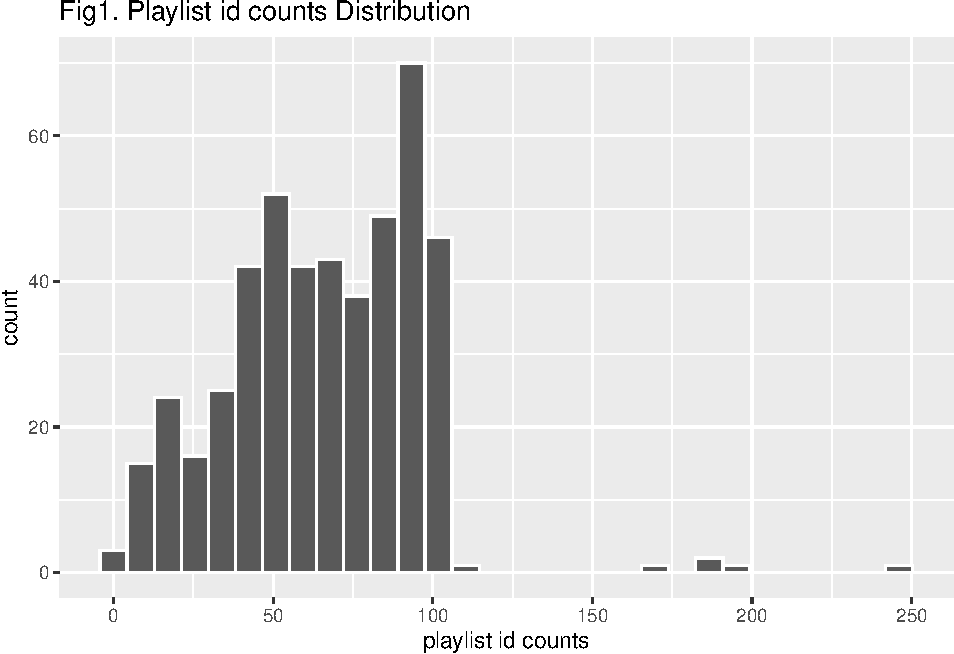
\includegraphics{Final-Report_files/figure-latex/unnamed-chunk-8-1.pdf}
\textbf{playlist\_name}

\begin{Shaded}
\begin{Highlighting}[]
\NormalTok{playlist\_name\_counts }\OtherTok{\textless{}{-}}\NormalTok{ spotify\_songs }\SpecialCharTok{\%\textgreater{}\%}
  \FunctionTok{count}\NormalTok{(playlist\_name) }\SpecialCharTok{\%\textgreater{}\%}
  \FunctionTok{arrange}\NormalTok{(}\FunctionTok{desc}\NormalTok{(n))}
\NormalTok{playlist\_name\_counts }\SpecialCharTok{\%\textgreater{}\%} \FunctionTok{ggplot}\NormalTok{(}\FunctionTok{aes}\NormalTok{(}\AttributeTok{x=}\NormalTok{ n)) }\SpecialCharTok{+} \FunctionTok{geom\_histogram}\NormalTok{(}\AttributeTok{bins =} \DecValTok{30}\NormalTok{, }\AttributeTok{color =} \StringTok{"white"}\NormalTok{) }\SpecialCharTok{+}
  \FunctionTok{ggtitle}\NormalTok{(}\StringTok{"Fig2. Playlist name counts Distribution"}\NormalTok{) }\SpecialCharTok{+}\FunctionTok{xlab}\NormalTok{(}\StringTok{"playlist name counts"}\NormalTok{) }\SpecialCharTok{+}\FunctionTok{ylab}\NormalTok{(}\StringTok{"count"}\NormalTok{)}
\end{Highlighting}
\end{Shaded}

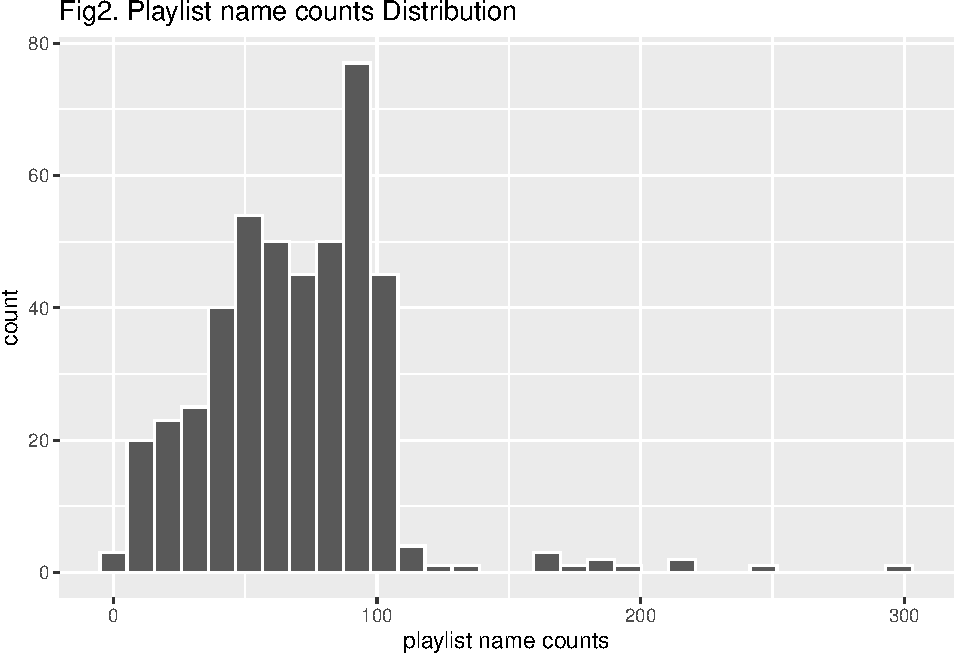
\includegraphics{Final-Report_files/figure-latex/unnamed-chunk-9-1.pdf}

\textbf{playlist\_subgenre}

\begin{Shaded}
\begin{Highlighting}[]
\NormalTok{playlist\_subgenre\_counts }\OtherTok{\textless{}{-}}\NormalTok{ spotify\_songs }\SpecialCharTok{\%\textgreater{}\%}
  \FunctionTok{count}\NormalTok{(playlist\_subgenre) }\SpecialCharTok{\%\textgreater{}\%}
  \FunctionTok{arrange}\NormalTok{(}\FunctionTok{desc}\NormalTok{(n))}

\NormalTok{playlist\_subgenre\_counts }\SpecialCharTok{\%\textgreater{}\%}
  \FunctionTok{ggplot}\NormalTok{(}\FunctionTok{aes}\NormalTok{(}\AttributeTok{x =}\NormalTok{ playlist\_subgenre, }\AttributeTok{y =}\NormalTok{ n)) }\SpecialCharTok{+}
  \FunctionTok{geom\_bar}\NormalTok{(}\AttributeTok{stat =} \StringTok{"identity"}\NormalTok{) }\SpecialCharTok{+}
  \FunctionTok{theme\_minimal}\NormalTok{() }\SpecialCharTok{+}
  \FunctionTok{theme}\NormalTok{(}\AttributeTok{axis.text.x =} \FunctionTok{element\_text}\NormalTok{(}\AttributeTok{angle =} \DecValTok{90}\NormalTok{, }\AttributeTok{vjust =} \FloatTok{0.5}\NormalTok{, }\AttributeTok{hjust =} \DecValTok{1}\NormalTok{)) }\SpecialCharTok{+}
  \FunctionTok{labs}\NormalTok{(}\AttributeTok{title =} \StringTok{"Fig3. SubGenre Counts in Playlist"}\NormalTok{,}
       \AttributeTok{x =} \StringTok{"Playlist SubGenre"}\NormalTok{,}
       \AttributeTok{y =} \StringTok{"Count"}\NormalTok{)}
\end{Highlighting}
\end{Shaded}

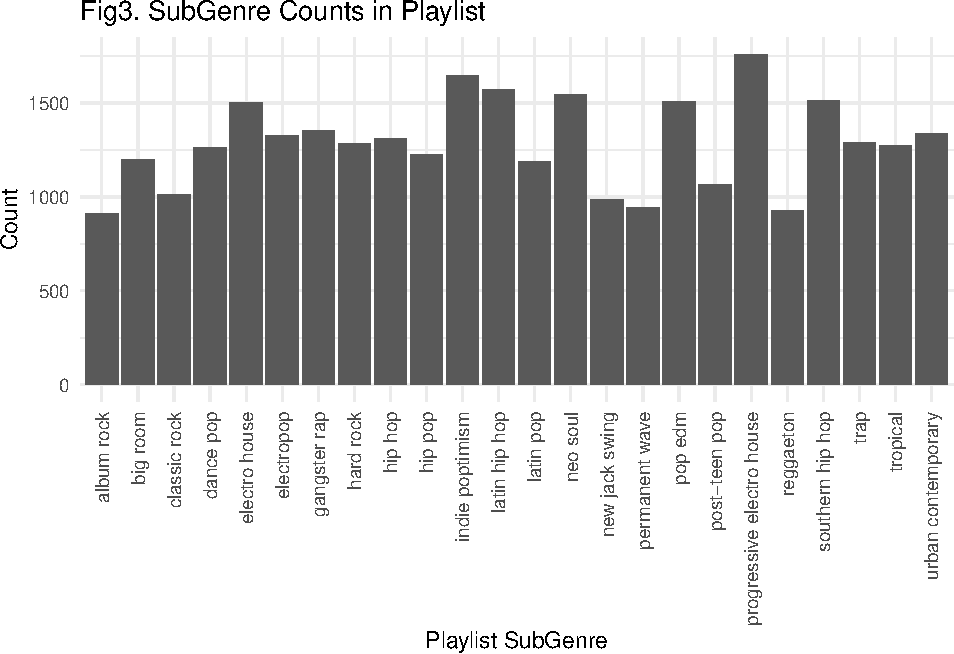
\includegraphics{Final-Report_files/figure-latex/unnamed-chunk-10-1.pdf}

\textbf{playlist\_genre (Response variable)}

\begin{Shaded}
\begin{Highlighting}[]
\NormalTok{playlist\_genre\_counts }\OtherTok{\textless{}{-}}\NormalTok{ spotify\_songs }\SpecialCharTok{\%\textgreater{}\%}
  \FunctionTok{count}\NormalTok{(playlist\_genre) }\SpecialCharTok{\%\textgreater{}\%}
  \FunctionTok{arrange}\NormalTok{(}\FunctionTok{desc}\NormalTok{(n))}

\NormalTok{playlist\_genre\_counts }\SpecialCharTok{\%\textgreater{}\%}
  \FunctionTok{ggplot}\NormalTok{(}\FunctionTok{aes}\NormalTok{(}\AttributeTok{x =}\NormalTok{ playlist\_genre, }\AttributeTok{y =}\NormalTok{ n)) }\SpecialCharTok{+}
  \FunctionTok{geom\_bar}\NormalTok{(}\AttributeTok{stat =} \StringTok{"identity"}\NormalTok{) }\SpecialCharTok{+}
  \FunctionTok{theme\_minimal}\NormalTok{() }\SpecialCharTok{+}
  \FunctionTok{labs}\NormalTok{(}\AttributeTok{title =} \StringTok{"Fig4. Genre Counts in Playlist"}\NormalTok{,}
       \AttributeTok{x =} \StringTok{"Playlist Genre"}\NormalTok{,}
       \AttributeTok{y =} \StringTok{"Count"}\NormalTok{)}
\end{Highlighting}
\end{Shaded}

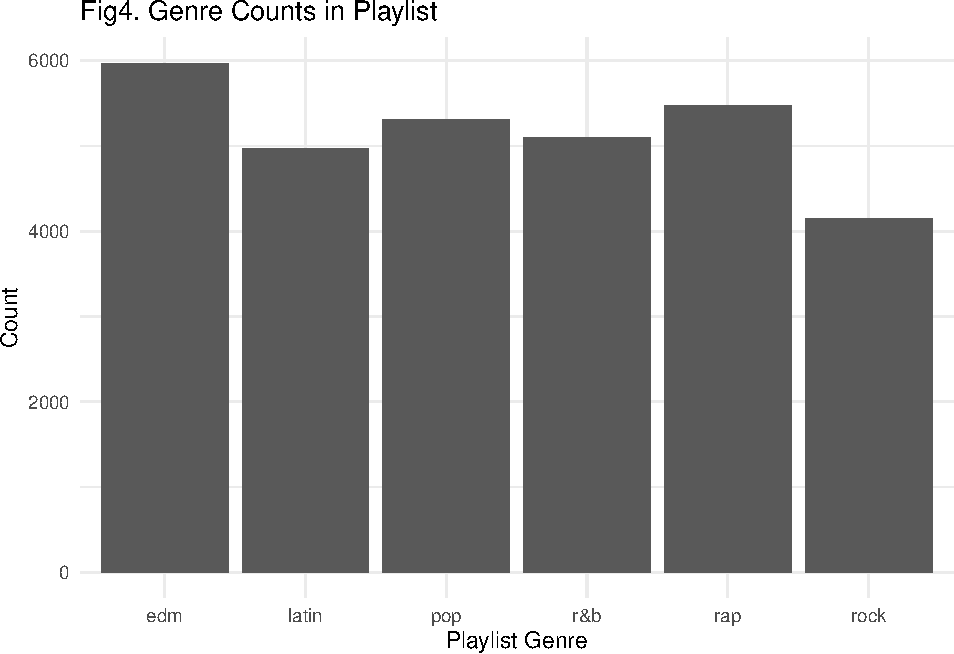
\includegraphics{Final-Report_files/figure-latex/unnamed-chunk-11-1.pdf}

\hypertarget{chi2-test-categorical-data-versus-categorical-data}{%
\paragraph{\texorpdfstring{\(Chi^2\)-Test (categorical data versus
categorical
data)}{Chi\^{}2-Test (categorical data versus categorical data)}}\label{chi2-test-categorical-data-versus-categorical-data}}

\begin{Shaded}
\begin{Highlighting}[]
\NormalTok{chisq\_test }\OtherTok{\textless{}{-}} \ControlFlowTok{function}\NormalTok{(variable\_name) \{}
\NormalTok{  contingency\_table }\OtherTok{\textless{}{-}}\NormalTok{ spotify\_songs }\SpecialCharTok{\%\textgreater{}\%}
    \FunctionTok{count}\NormalTok{(}\SpecialCharTok{!!}\FunctionTok{sym}\NormalTok{(variable\_name), playlist\_genre) }\SpecialCharTok{\%\textgreater{}\%}
    \FunctionTok{spread}\NormalTok{(}\AttributeTok{key =}\NormalTok{ playlist\_genre, }\AttributeTok{value =}\NormalTok{ n, }\AttributeTok{fill =} \DecValTok{0}\NormalTok{) }\SpecialCharTok{\%\textgreater{}\%}
    \FunctionTok{column\_to\_rownames}\NormalTok{(}\AttributeTok{var=}\NormalTok{ variable\_name)}
  
\NormalTok{  chi\_square\_test }\OtherTok{\textless{}{-}} \FunctionTok{chisq.test}\NormalTok{(contingency\_table)}
  \FunctionTok{cat}\NormalTok{(variable\_name)}
  \FunctionTok{print}\NormalTok{(chi\_square\_test)}
\NormalTok{\}}

\ControlFlowTok{for}\NormalTok{ (variable }\ControlFlowTok{in} \FunctionTok{setdiff}\NormalTok{(categorical\_variables, }\StringTok{"playlist\_genre"}\NormalTok{)) \{}
  \FunctionTok{chisq\_test}\NormalTok{(variable)}
\NormalTok{\}}
\end{Highlighting}
\end{Shaded}

\begin{verbatim}
## Warning in chisq.test(contingency_table): Chi-squared approximation may be
## incorrect
\end{verbatim}

\begin{verbatim}
## playlist_name
##  Pearson's Chi-squared test
## 
## data:  contingency_table
## X-squared = 152976, df = 2240, p-value < 2.2e-16
\end{verbatim}

\begin{verbatim}
## Warning in chisq.test(contingency_table): Chi-squared approximation may be
## incorrect
\end{verbatim}

\begin{verbatim}
## playlist_id
##  Pearson's Chi-squared test
## 
## data:  contingency_table
## X-squared = 152976, df = 2350, p-value < 2.2e-16
## 
## playlist_subgenre
##  Pearson's Chi-squared test
## 
## data:  contingency_table
## X-squared = 154735, df = 115, p-value < 2.2e-16
\end{verbatim}

\begin{Shaded}
\begin{Highlighting}[]
\NormalTok{spotify\_songs }\OtherTok{\textless{}{-}}\NormalTok{ spotify\_songs }\SpecialCharTok{\%\textgreater{}\%} 
\NormalTok{  dplyr}\SpecialCharTok{::}\FunctionTok{select}\NormalTok{(}\SpecialCharTok{{-}}\FunctionTok{setdiff}\NormalTok{(categorical\_variables, }\StringTok{"playlist\_genre"}\NormalTok{))}
\end{Highlighting}
\end{Shaded}

\hypertarget{numerical-variable}{%
\subsection{Numerical variable}\label{numerical-variable}}

\textbf{Compile a standard function for EDA}

\begin{itemize}
\tightlist
\item
  plot a histogram to check the distribution of each numerical variable
\item
  plot a box plot to check the distribution of each numerical variable
  in different genres
\item
  Anova test to check the distribution differences in different genres
\end{itemize}

\begin{Shaded}
\begin{Highlighting}[]
\NormalTok{analyze\_variable\_hist }\OtherTok{\textless{}{-}} \ControlFlowTok{function}\NormalTok{(variable\_name) \{}
  
  \CommentTok{\# histogram}
\NormalTok{  idx }\OtherTok{=} \DecValTok{4} \SpecialCharTok{+} \DecValTok{2}\SpecialCharTok{*}\FunctionTok{which}\NormalTok{(numerical\_variables }\SpecialCharTok{==}\NormalTok{ variable\_name)}\SpecialCharTok{{-}}\DecValTok{1}
\NormalTok{  histo\_gram }\OtherTok{\textless{}{-}}\NormalTok{ spotify\_songs }\SpecialCharTok{\%\textgreater{}\%} \FunctionTok{ggplot}\NormalTok{(}\FunctionTok{aes\_string}\NormalTok{(variable\_name)) }\SpecialCharTok{+} 
    \FunctionTok{geom\_histogram}\NormalTok{(}\AttributeTok{bins =} \DecValTok{30}\NormalTok{,}\AttributeTok{color=}\StringTok{"white"}\NormalTok{) }\SpecialCharTok{+}
    \FunctionTok{ggtitle}\NormalTok{(}\FunctionTok{paste}\NormalTok{(}\StringTok{"Fig"}\NormalTok{,idx,}\StringTok{". Histogram of"}\NormalTok{, variable\_name)) }\SpecialCharTok{+} 
    \FunctionTok{xlab}\NormalTok{(variable\_name) }\SpecialCharTok{+} \FunctionTok{ylab}\NormalTok{(}\StringTok{"count"}\NormalTok{)}
  \FunctionTok{print}\NormalTok{(histo\_gram)}
  
\NormalTok{\}}

\NormalTok{analyze\_variable\_box }\OtherTok{\textless{}{-}} \ControlFlowTok{function}\NormalTok{(variable\_name) \{}
\CommentTok{\# boxplot}
\NormalTok{  idx }\OtherTok{=} \DecValTok{4} \SpecialCharTok{+} \DecValTok{2}\SpecialCharTok{*}\FunctionTok{which}\NormalTok{(numerical\_variables }\SpecialCharTok{==}\NormalTok{ variable\_name)}
\NormalTok{  box\_plot }\OtherTok{\textless{}{-}}\NormalTok{ spotify\_songs }\SpecialCharTok{\%\textgreater{}\%} \FunctionTok{ggplot}\NormalTok{(}\FunctionTok{aes\_string}\NormalTok{(}\AttributeTok{x =} \StringTok{"playlist\_genre"}\NormalTok{, }
                                                  \AttributeTok{y =}\NormalTok{ variable\_name,}
                                                  \AttributeTok{fill =} \StringTok{"playlist\_genre"}\NormalTok{)) }\SpecialCharTok{+}
    \FunctionTok{geom\_boxplot}\NormalTok{() }\SpecialCharTok{+} \FunctionTok{ggtitle}\NormalTok{(}\FunctionTok{paste}\NormalTok{(}\StringTok{"Fig"}\NormalTok{,idx,}\StringTok{". Distribution of"}\NormalTok{, variable\_name, }\StringTok{"in different genres"}\NormalTok{)) }\SpecialCharTok{+} 
    \FunctionTok{xlab}\NormalTok{(}\StringTok{"Genres"}\NormalTok{) }\SpecialCharTok{+} \FunctionTok{ylab}\NormalTok{(}\FunctionTok{paste}\NormalTok{(}\StringTok{"Distribution of"}\NormalTok{, variable\_name))}
  \FunctionTok{print}\NormalTok{(box\_plot)}
\NormalTok{\}}

\NormalTok{analyze\_variable\_ANOVA }\OtherTok{\textless{}{-}} \ControlFlowTok{function}\NormalTok{(variable\_name) \{}
  \CommentTok{\#ANOVA}
\NormalTok{  avg\_by\_genre }\OtherTok{\textless{}{-}} \FunctionTok{tapply}\NormalTok{(spotify\_songs[[variable\_name]], spotify\_songs}\SpecialCharTok{$}\NormalTok{playlist\_genre, mean)}
  \FunctionTok{print}\NormalTok{(avg\_by\_genre)}
  
\NormalTok{  formula\_str }\OtherTok{\textless{}{-}} \FunctionTok{paste}\NormalTok{(variable\_name, }\StringTok{"\textasciitilde{} playlist\_genre"}\NormalTok{)}
\NormalTok{  anova\_result }\OtherTok{\textless{}{-}} \FunctionTok{aov}\NormalTok{(}\FunctionTok{as.formula}\NormalTok{(formula\_str), }\AttributeTok{data =}\NormalTok{ spotify\_songs)}
  \FunctionTok{print}\NormalTok{(}\FunctionTok{summary}\NormalTok{(anova\_result))}
  
\NormalTok{  tukey\_result }\OtherTok{\textless{}{-}} \FunctionTok{TukeyHSD}\NormalTok{(anova\_result)}
  \FunctionTok{print}\NormalTok{(tukey\_result)}
\NormalTok{\}}
\end{Highlighting}
\end{Shaded}

\begin{Shaded}
\begin{Highlighting}[]
\ControlFlowTok{for}\NormalTok{ (variable }\ControlFlowTok{in}\NormalTok{ numerical\_variables) \{}
  \FunctionTok{cat}\NormalTok{(}\StringTok{"}\SpecialCharTok{\textbackslash{}n}\StringTok{"}\NormalTok{)}
  \FunctionTok{cat}\NormalTok{(}\StringTok{"}\SpecialCharTok{\textbackslash{}n}\StringTok{"}\NormalTok{)}
  \FunctionTok{analyze\_variable\_hist}\NormalTok{(variable)}
  \FunctionTok{cat}\NormalTok{(}\StringTok{"}\SpecialCharTok{\textbackslash{}n}\StringTok{"}\NormalTok{)}
  \FunctionTok{cat}\NormalTok{(}\StringTok{"}\SpecialCharTok{\textbackslash{}n}\StringTok{"}\NormalTok{)}
  \FunctionTok{analyze\_variable\_box}\NormalTok{(variable)}
  \FunctionTok{cat}\NormalTok{(}\StringTok{"}\SpecialCharTok{\textbackslash{}n}\StringTok{"}\NormalTok{)}
  \FunctionTok{cat}\NormalTok{(variable)}
  \FunctionTok{cat}\NormalTok{(}\StringTok{"}\SpecialCharTok{\textbackslash{}n}\StringTok{"}\NormalTok{)}
  \FunctionTok{analyze\_variable\_ANOVA}\NormalTok{ (variable)}
  \FunctionTok{print}\NormalTok{(}\StringTok{"NEXT\textgreater{}\textgreater{}\textgreater{}\textgreater{}NEXT\textgreater{}\textgreater{}\textgreater{}\textgreater{}NEXT\textgreater{}\textgreater{}\textgreater{}\textgreater{}NEXT\textgreater{}\textgreater{}\textgreater{}\textgreater{}NEXT\textgreater{}\textgreater{}\textgreater{}\textgreater{}NEXT\textgreater{}\textgreater{}\textgreater{}\textgreater{}NEXT\textgreater{}\textgreater{}\textgreater{}\textgreater{}"}\NormalTok{)}
\NormalTok{\}}
\end{Highlighting}
\end{Shaded}

\begin{verbatim}
## Warning: `aes_string()` was deprecated in ggplot2 3.0.0.
## i Please use tidy evaluation ideoms with `aes()`
\end{verbatim}

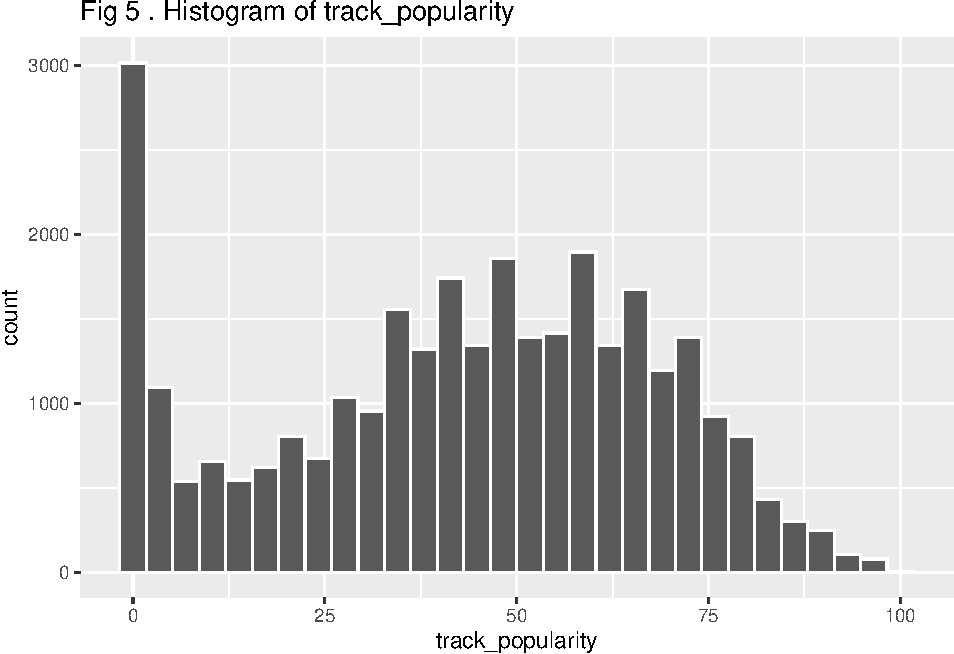
\includegraphics{Final-Report_files/figure-latex/unnamed-chunk-14-1.pdf}

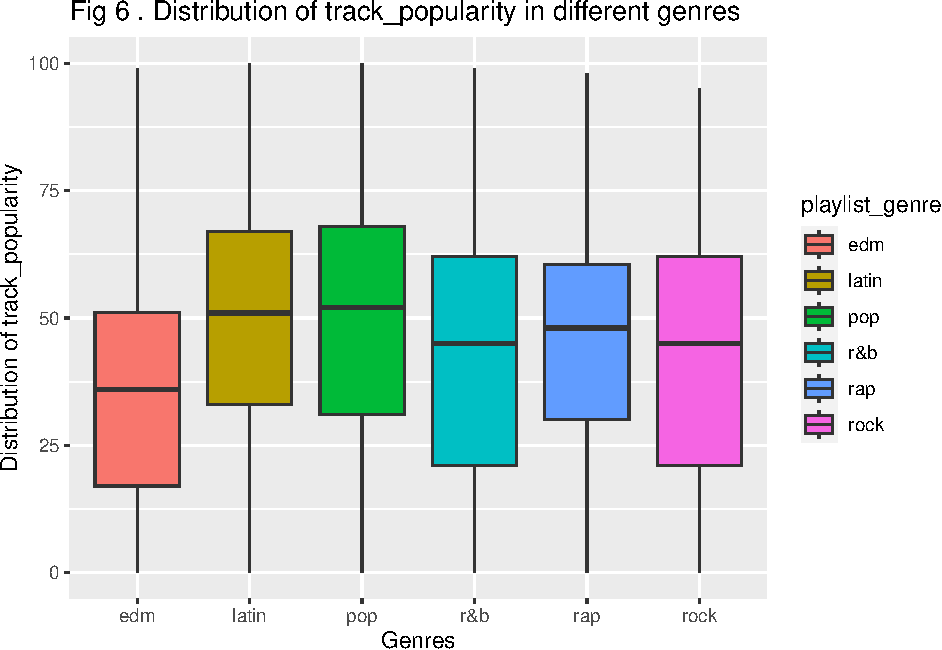
\includegraphics{Final-Report_files/figure-latex/unnamed-chunk-14-2.pdf}

\begin{verbatim}
## 
## track_popularity
##      edm    latin      pop      r&b      rap     rock 
## 34.93885 47.56679 48.07147 41.81017 43.62128 41.42247 
##                   Df   Sum Sq Mean Sq F value Pr(>F)    
## playlist_genre     5   645473  129095   214.4 <2e-16 ***
## Residuals      30941 18627072     602                   
## ---
## Signif. codes:  0 '***' 0.001 '**' 0.01 '*' 0.05 '.' 0.1 ' ' 1
##   Tukey multiple comparisons of means
##     95% family-wise confidence level
## 
## Fit: aov(formula = as.formula(formula_str), data = spotify_songs)
## 
## $playlist_genre
##                  diff        lwr        upr     p adj
## latin-edm  12.6279435 11.2847705 13.9711166 0.0000000
## pop-edm    13.1326183 11.8131651 14.4520714 0.0000000
## r&b-edm     6.8713181  5.5376085  8.2050277 0.0000000
## rap-edm     8.6824251  7.3737436  9.9911066 0.0000000
## rock-edm    6.4836233  5.0701367  7.8971099 0.0000000
## pop-latin   0.5046747 -0.8762588  1.8856082 0.9039405
## r&b-latin  -5.7566255 -7.1511871 -4.3620638 0.0000000
## rap-latin  -3.9455185 -5.3161635 -2.5748734 0.0000000
## rock-latin -6.1443202 -7.6153624 -4.6732780 0.0000000
## r&b-pop    -6.2613002 -7.6330308 -4.8895695 0.0000000
## rap-pop    -4.4501932 -5.7976020 -3.1027843 0.0000000
## rock-pop   -6.6489949 -8.0984113 -5.1995785 0.0000000
## rap-r&b     1.8111070  0.4497344  3.1724796 0.0020783
## rock-r&b   -0.3876947 -1.8501012  1.0747117 0.9747460
## rock-rap   -2.1988017 -3.6384192 -0.7591843 0.0001952
## 
## [1] "NEXT>>>>NEXT>>>>NEXT>>>>NEXT>>>>NEXT>>>>NEXT>>>>NEXT>>>>"
\end{verbatim}

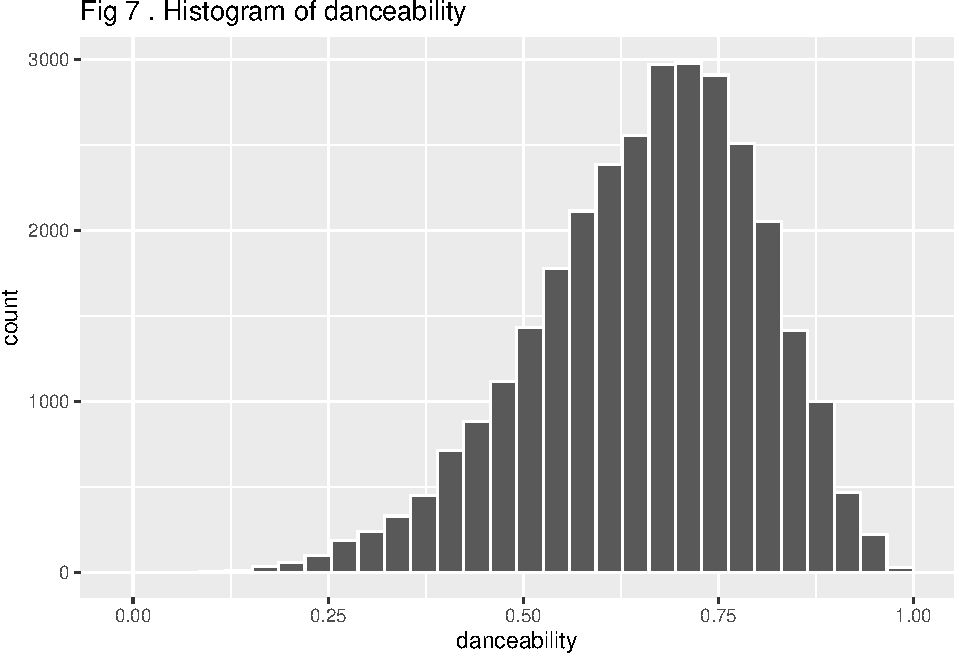
\includegraphics{Final-Report_files/figure-latex/unnamed-chunk-14-3.pdf}

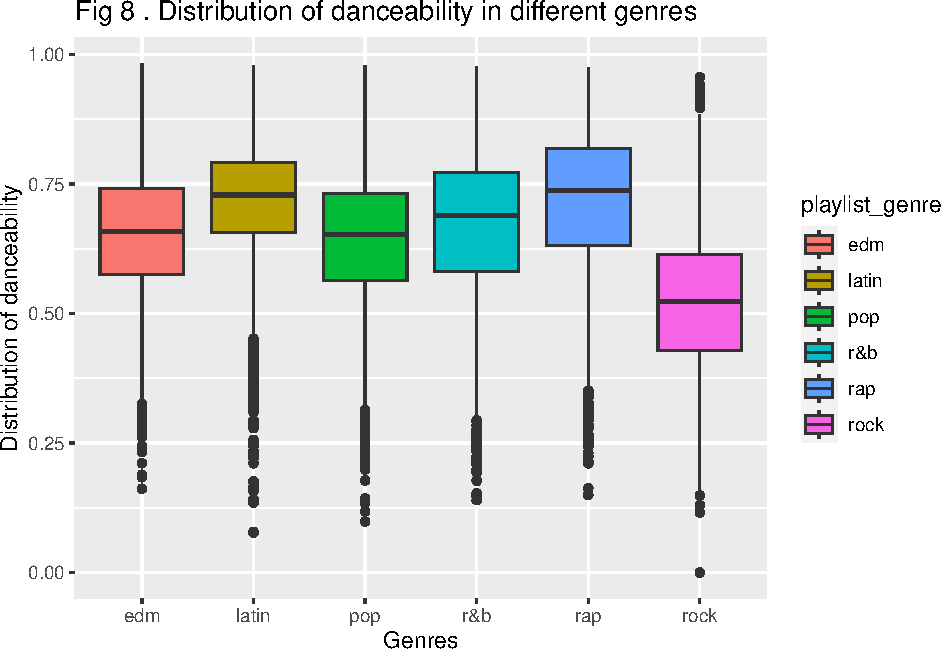
\includegraphics{Final-Report_files/figure-latex/unnamed-chunk-14-4.pdf}

\begin{verbatim}
## 
## danceability
##       edm     latin       pop       r&b       rap      rock 
## 0.6546405 0.7134672 0.6406509 0.6697148 0.7175184 0.5201989 
##                   Df Sum Sq Mean Sq F value Pr(>F)    
## playlist_genre     5  115.7  23.149    1364 <2e-16 ***
## Residuals      30941  525.3   0.017                   
## ---
## Signif. codes:  0 '***' 0.001 '**' 0.01 '*' 0.05 '.' 0.1 ' ' 1
##   Tukey multiple comparisons of means
##     95% family-wise confidence level
## 
## Fit: aov(formula = as.formula(formula_str), data = spotify_songs)
## 
## $playlist_genre
##                    diff          lwr          upr     p adj
## latin-edm   0.058826742  0.051694070  0.065959414 0.0000000
## pop-edm    -0.013989618 -0.020996330 -0.006982906 0.0000002
## r&b-edm     0.015074287  0.007991868  0.022156705 0.0000000
## rap-edm     0.062877894  0.055928383  0.069827405 0.0000000
## rock-edm   -0.134441537 -0.141947596 -0.126935478 0.0000000
## pop-latin  -0.072816359 -0.080149551 -0.065483168 0.0000000
## r&b-latin  -0.043752455 -0.051158016 -0.036346894 0.0000000
## rap-latin   0.004051152 -0.003227405  0.011329709 0.6077803
## rock-latin -0.193268278 -0.201079976 -0.185456581 0.0000000
## r&b-pop     0.029063904  0.021779583  0.036348226 0.0000000
## rap-pop     0.076867512  0.069712346  0.084022677 0.0000000
## rock-pop   -0.120451919 -0.128148776 -0.112755062 0.0000000
## rap-r&b     0.047803607  0.040574290  0.055032925 0.0000000
## rock-r&b   -0.149515823 -0.157281662 -0.141749985 0.0000000
## rock-rap   -0.197319431 -0.204964253 -0.189674609 0.0000000
## 
## [1] "NEXT>>>>NEXT>>>>NEXT>>>>NEXT>>>>NEXT>>>>NEXT>>>>NEXT>>>>"
\end{verbatim}

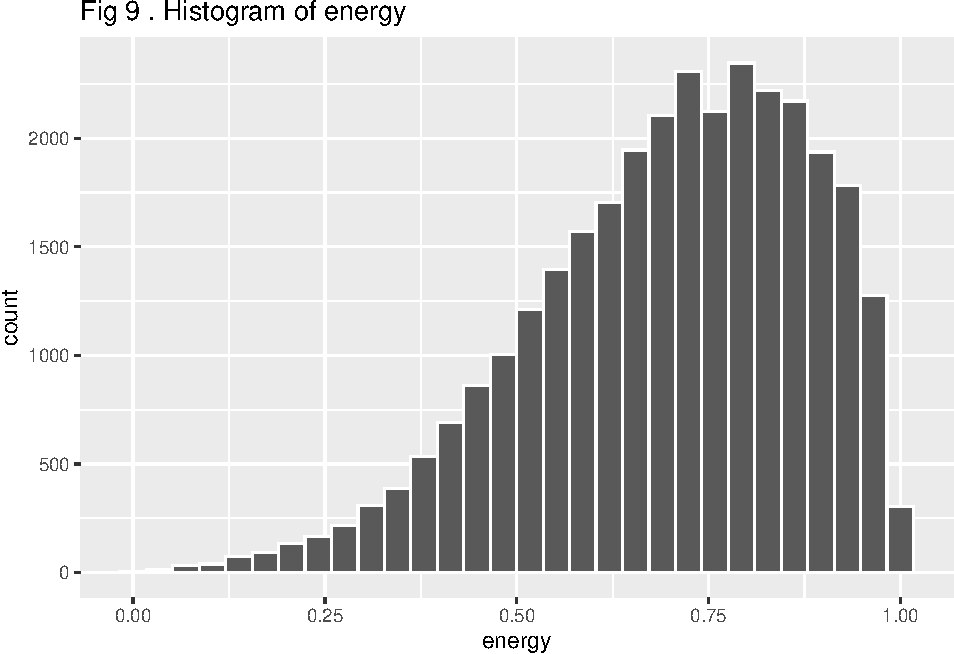
\includegraphics{Final-Report_files/figure-latex/unnamed-chunk-14-5.pdf}

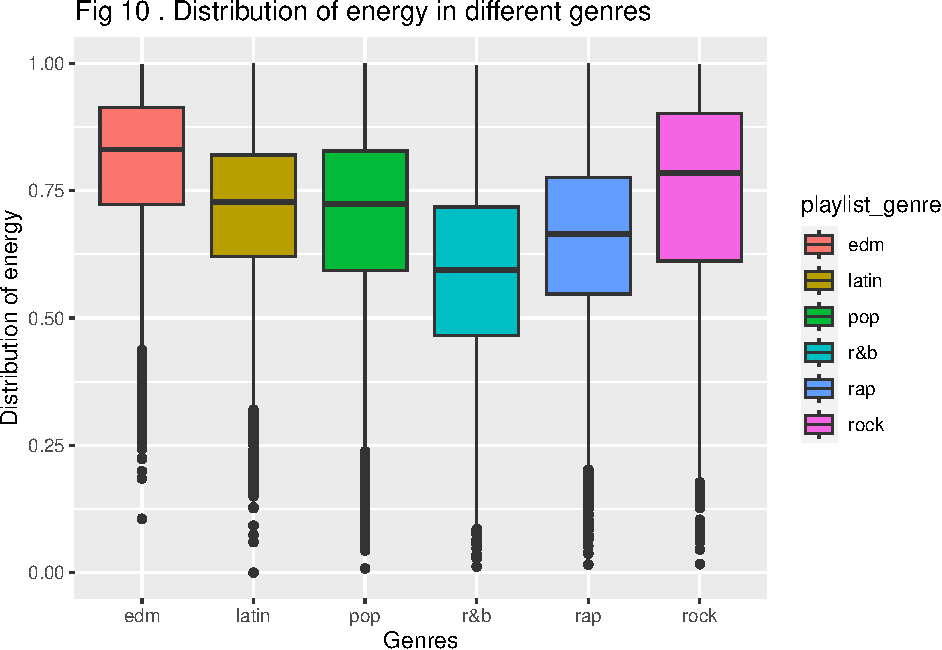
\includegraphics{Final-Report_files/figure-latex/unnamed-chunk-14-6.pdf}

\begin{verbatim}
## 
## energy
##       edm     latin       pop       r&b       rap      rock 
## 0.8029283 0.7076550 0.6983240 0.5889020 0.6502701 0.7385113 
##                   Df Sum Sq Mean Sq F value Pr(>F)    
## playlist_genre     5  146.1  29.212    1045 <2e-16 ***
## Residuals      30941  864.6   0.028                   
## ---
## Signif. codes:  0 '***' 0.001 '**' 0.01 '*' 0.05 '.' 0.1 ' ' 1
##   Tukey multiple comparisons of means
##     95% family-wise confidence level
## 
## Fit: aov(formula = as.formula(formula_str), data = spotify_songs)
## 
## $playlist_genre
##                   diff         lwr           upr     p adj
## latin-edm  -0.09527329 -0.10442416 -0.0861224264 0.0000000
## pop-edm    -0.10460426 -0.11359353 -0.0956149974 0.0000000
## r&b-edm    -0.21402625 -0.22311265 -0.2049398600 0.0000000
## rap-edm    -0.15265824 -0.16157412 -0.1437423549 0.0000000
## rock-edm   -0.06441699 -0.07404689 -0.0547870819 0.0000000
## pop-latin  -0.00933097 -0.01873910  0.0000771546 0.0533869
## r&b-latin  -0.11875296 -0.12825393 -0.1092519889 0.0000000
## rap-latin  -0.05738494 -0.06672297 -0.0480469105 0.0000000
## rock-latin  0.03085631  0.02083428  0.0408783312 0.0000000
## r&b-pop    -0.10942199 -0.11876742 -0.1000765634 0.0000000
## rap-pop    -0.04805397 -0.05723370 -0.0388742455 0.0000000
## rock-pop    0.04018728  0.03031259  0.0500619677 0.0000000
## rap-r&b     0.06136802  0.05209316  0.0706428778 0.0000000
## rock-r&b    0.14960927  0.13964608  0.1595724573 0.0000000
## rock-rap    0.08824125  0.07843332  0.0980491802 0.0000000
## 
## [1] "NEXT>>>>NEXT>>>>NEXT>>>>NEXT>>>>NEXT>>>>NEXT>>>>NEXT>>>>"
\end{verbatim}

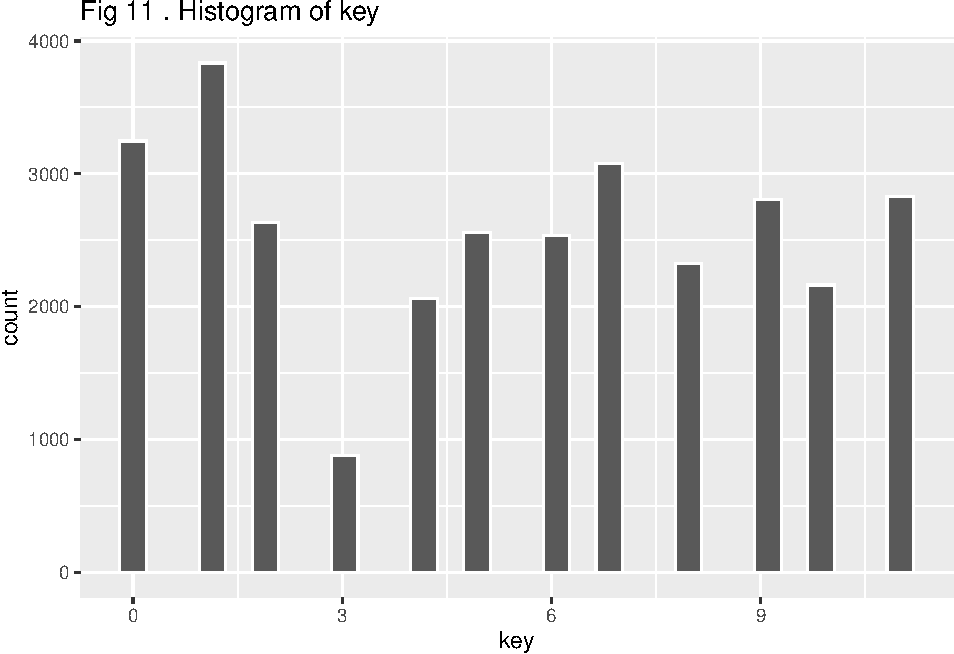
\includegraphics{Final-Report_files/figure-latex/unnamed-chunk-14-7.pdf}

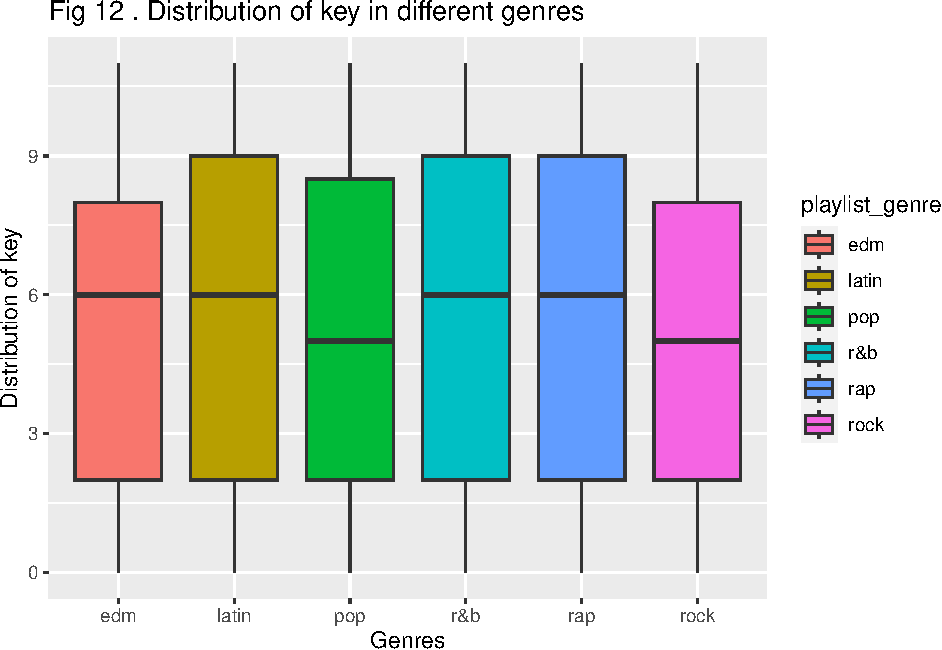
\includegraphics{Final-Report_files/figure-latex/unnamed-chunk-14-8.pdf}

\begin{verbatim}
## 
## key
##      edm    latin      pop      r&b      rap     rock 
## 5.351148 5.481161 5.301150 5.390459 5.455675 5.203279 
##                   Df Sum Sq Mean Sq F value  Pr(>F)   
## playlist_genre     5    246   49.22    3.77 0.00206 **
## Residuals      30941 403958   13.06                   
## ---
## Signif. codes:  0 '***' 0.001 '**' 0.01 '*' 0.05 '.' 0.1 ' ' 1
##   Tukey multiple comparisons of means
##     95% family-wise confidence level
## 
## Fit: aov(formula = as.formula(formula_str), data = spotify_songs)
## 
## $playlist_genre
##                   diff         lwr         upr     p adj
## latin-edm   0.13001299 -0.06778771  0.32781369 0.4188392
## pop-edm    -0.04999730 -0.24430492  0.14431031 0.9778599
## r&b-edm     0.03931177 -0.15709531  0.23571885 0.9929300
## rap-edm     0.10452778 -0.08819355  0.29724912 0.6345533
## rock-edm   -0.14786812 -0.35602345  0.06028722 0.3282987
## pop-latin  -0.18001030 -0.38337174  0.02335115 0.1175059
## r&b-latin  -0.09070122 -0.29606959  0.11466714 0.8075283
## rap-latin  -0.02548521 -0.22733154  0.17636112 0.9992140
## rock-latin -0.27788111 -0.49451229 -0.06124993 0.0034988
## r&b-pop     0.08930907 -0.11269712  0.29131526 0.8068408
## rap-pop     0.15452509 -0.04389939  0.35294957 0.2287320
## rock-pop   -0.09787081 -0.31131730  0.11557567 0.7815225
## rap-r&b     0.06521602 -0.13526482  0.26569685 0.9396816
## rock-r&b   -0.18717988 -0.40253934  0.02817957 0.1309320
## rock-rap   -0.25239590 -0.46439936 -0.04039244 0.0090504
## 
## [1] "NEXT>>>>NEXT>>>>NEXT>>>>NEXT>>>>NEXT>>>>NEXT>>>>NEXT>>>>"
\end{verbatim}

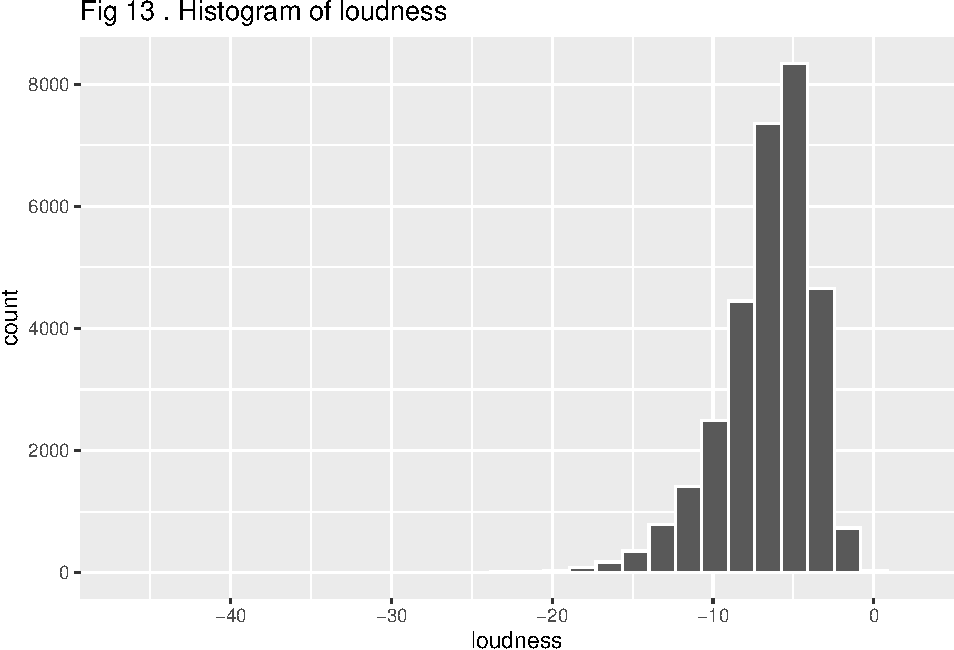
\includegraphics{Final-Report_files/figure-latex/unnamed-chunk-14-9.pdf}

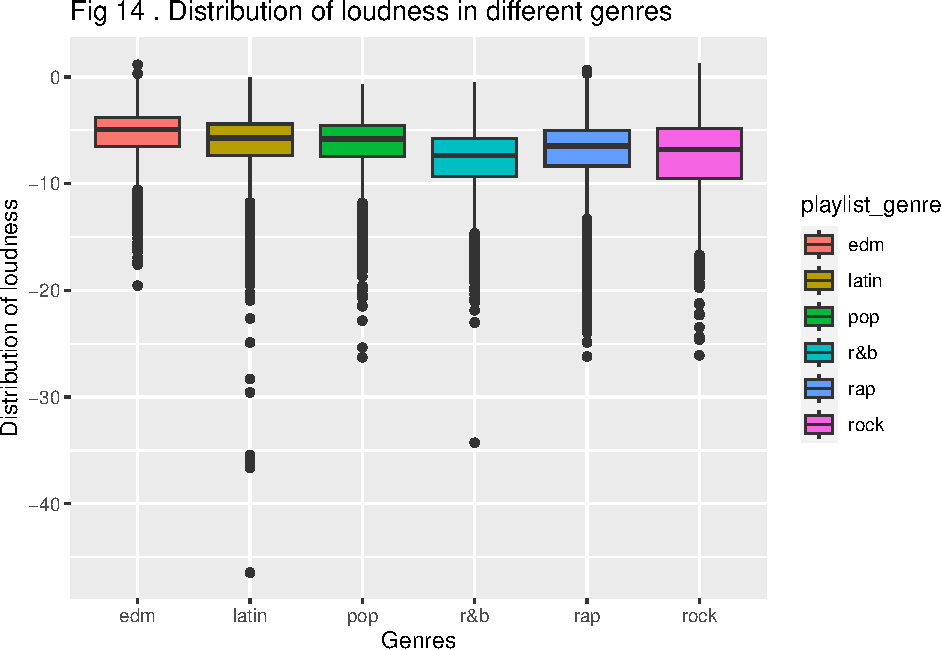
\includegraphics{Final-Report_files/figure-latex/unnamed-chunk-14-10.pdf}

\begin{verbatim}
## 
## loudness
##       edm     latin       pop       r&b       rap      rock 
## -5.411837 -6.222340 -6.300329 -7.807318 -7.013525 -7.410332 
##                   Df Sum Sq Mean Sq F value Pr(>F)    
## playlist_genre     5  20647    4129   514.2 <2e-16 ***
## Residuals      30941 248461       8                   
## ---
## Signif. codes:  0 '***' 0.001 '**' 0.01 '*' 0.05 '.' 0.1 ' ' 1
##   Tukey multiple comparisons of means
##     95% family-wise confidence level
## 
## Fit: aov(formula = as.formula(formula_str), data = spotify_songs)
## 
## $playlist_genre
##                   diff        lwr         upr    p adj
## latin-edm  -0.81050326 -0.9656307 -0.65537584 0.000000
## pop-edm    -0.88849278 -1.0408807 -0.73610485 0.000000
## r&b-edm    -2.39548156 -2.5495160 -2.24144711 0.000000
## rap-edm    -1.60168884 -1.7528327 -1.45054497 0.000000
## rock-edm   -1.99849539 -2.1617435 -1.83524724 0.000000
## pop-latin  -0.07798952 -0.2374780  0.08149897 0.731055
## r&b-latin  -1.58497830 -1.7460407 -1.42391586 0.000000
## rap-latin  -0.79118558 -0.9494858 -0.63288533 0.000000
## rock-latin -1.18799213 -1.3578876 -1.01809670 0.000000
## r&b-pop    -1.50698878 -1.6654144 -1.34856316 0.000000
## rap-pop    -0.71319606 -0.8688127 -0.55757944 0.000000
## rock-pop   -1.11000261 -1.2774004 -0.94260481 0.000000
## rap-r&b     0.79379272  0.6365634  0.95102206 0.000000
## rock-r&b    0.39698617  0.2280881  0.56588423 0.000000
## rock-rap   -0.39680655 -0.5630726 -0.23054046 0.000000
## 
## [1] "NEXT>>>>NEXT>>>>NEXT>>>>NEXT>>>>NEXT>>>>NEXT>>>>NEXT>>>>"
\end{verbatim}

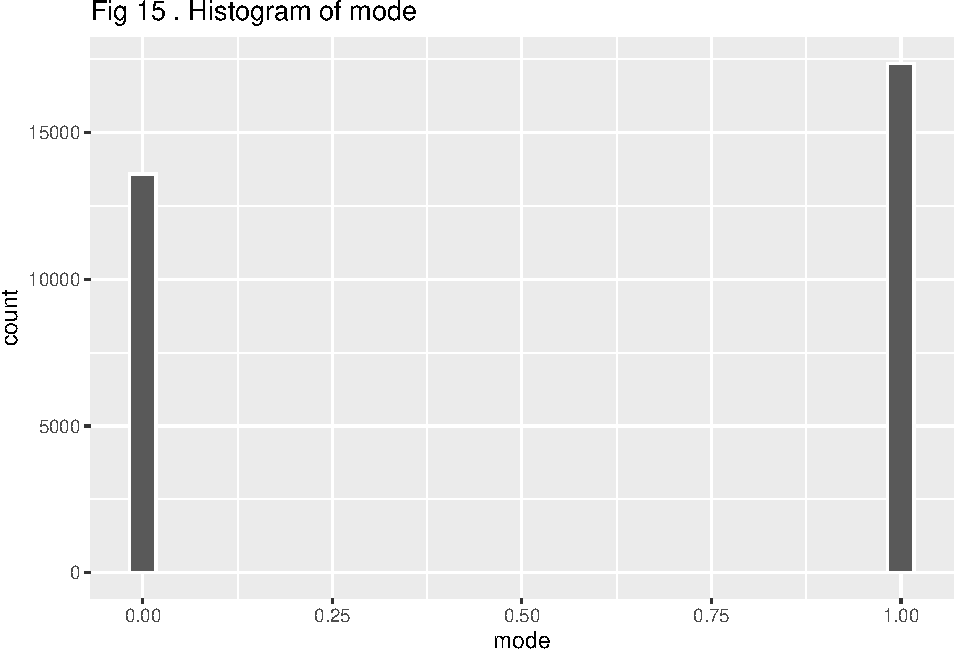
\includegraphics{Final-Report_files/figure-latex/unnamed-chunk-14-11.pdf}

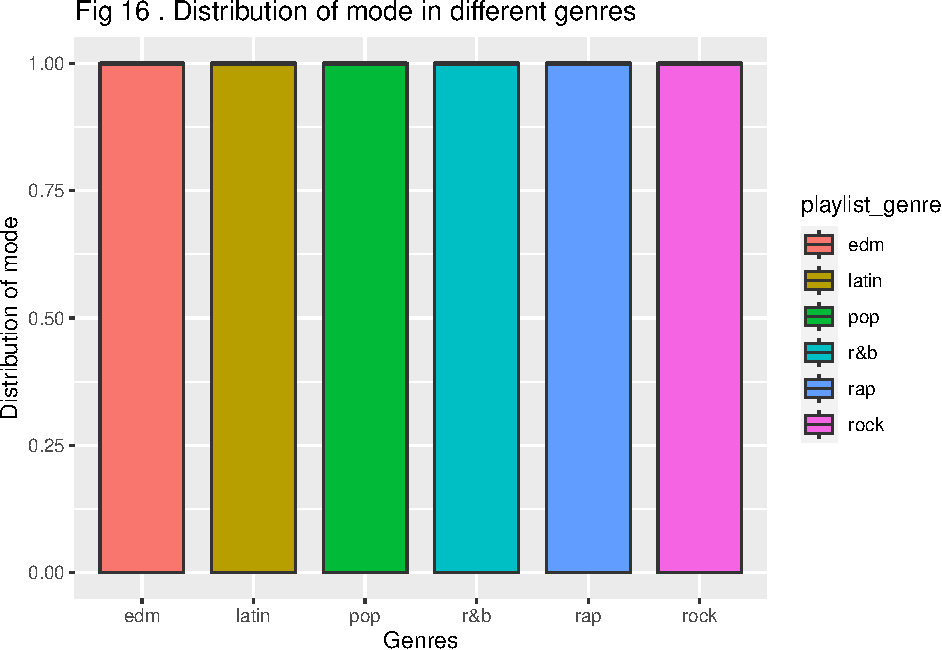
\includegraphics{Final-Report_files/figure-latex/unnamed-chunk-14-12.pdf}

\begin{verbatim}
## 
## mode
##       edm     latin       pop       r&b       rap      rock 
## 0.5191824 0.5617570 0.5855176 0.5188457 0.5189179 0.6956836 
##                   Df Sum Sq Mean Sq F value Pr(>F)    
## playlist_genre     5    108  21.519   88.61 <2e-16 ***
## Residuals      30941   7514   0.243                   
## ---
## Signif. codes:  0 '***' 0.001 '**' 0.01 '*' 0.05 '.' 0.1 ' ' 1
##   Tukey multiple comparisons of means
##     95% family-wise confidence level
## 
## Fit: aov(formula = as.formula(formula_str), data = spotify_songs)
## 
## $playlist_genre
##                     diff          lwr         upr     p adj
## latin-edm   4.257456e-02  0.015596958  0.06955216 0.0001005
## pop-edm     6.633519e-02  0.039834002  0.09283638 0.0000000
## r&b-edm    -3.367418e-04 -0.027124270  0.02645079 1.0000000
## rap-edm    -2.645117e-04 -0.026549350  0.02602033 1.0000000
## rock-edm    1.765012e-01  0.148111338  0.20489103 0.0000000
## pop-latin   2.376063e-02 -0.003975389  0.05149665 0.1421710
## r&b-latin  -4.291130e-02 -0.070921040 -0.01490156 0.0001838
## rap-latin  -4.283907e-02 -0.070368446 -0.01530970 0.0001344
## rock-latin  1.339266e-01  0.104380776  0.16347247 0.0000000
## r&b-pop    -6.667193e-02 -0.094223109 -0.03912075 0.0000000
## rap-pop    -6.659970e-02 -0.093662378 -0.03953702 0.0000000
## rock-pop    1.101660e-01  0.081054500  0.13927749 0.0000000
## rap-r&b     7.223008e-05 -0.027270908  0.02741537 1.0000000
## rock-r&b    1.768379e-01  0.147465526  0.20621033 0.0000000
## rock-rap    1.767657e-01  0.147851012  0.20568038 0.0000000
## 
## [1] "NEXT>>>>NEXT>>>>NEXT>>>>NEXT>>>>NEXT>>>>NEXT>>>>NEXT>>>>"
\end{verbatim}

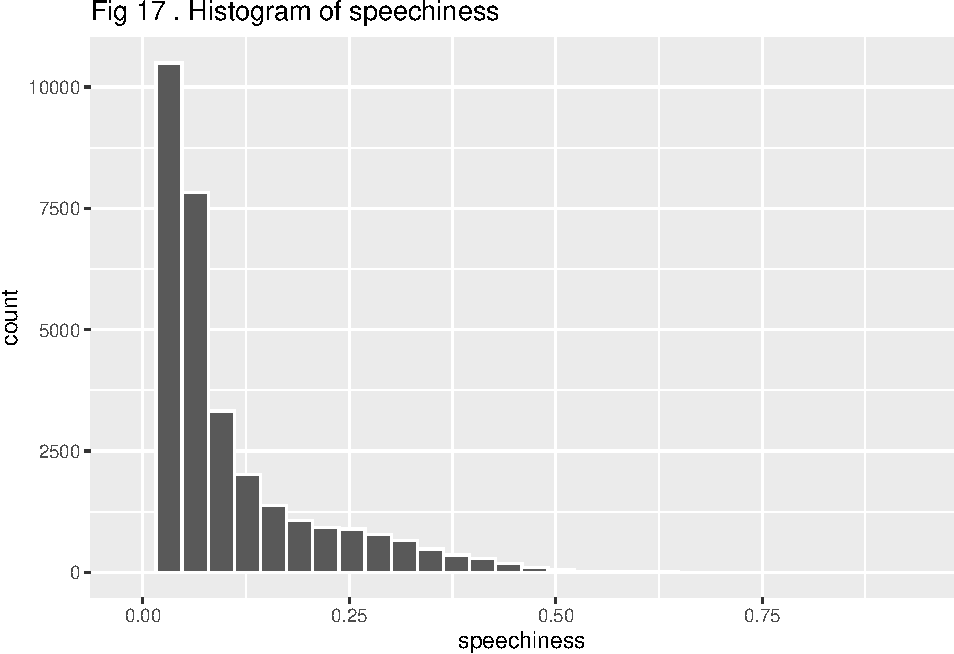
\includegraphics{Final-Report_files/figure-latex/unnamed-chunk-14-13.pdf}

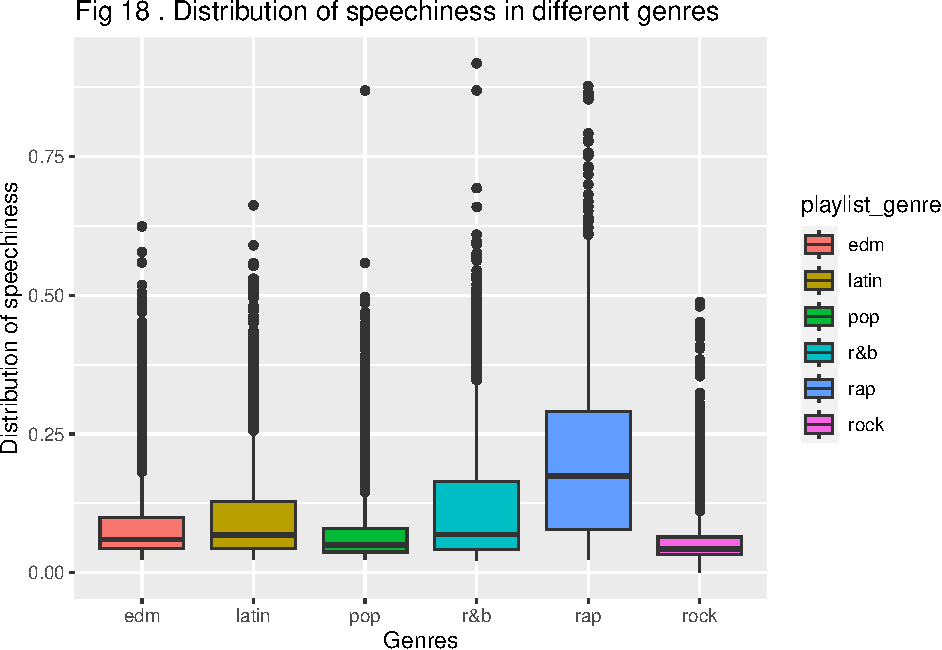
\includegraphics{Final-Report_files/figure-latex/unnamed-chunk-14-14.pdf}

\begin{verbatim}
## 
## speechiness
##        edm      latin        pop        r&b        rap       rock 
## 0.08687212 0.10327175 0.07482399 0.11890188 0.19613449 0.05865602 
##                   Df Sum Sq Mean Sq F value Pr(>F)    
## playlist_genre     5  61.81  12.362    1478 <2e-16 ***
## Residuals      30941 258.76   0.008                   
## ---
## Signif. codes:  0 '***' 0.001 '**' 0.01 '*' 0.05 '.' 0.1 ' ' 1
##   Tukey multiple comparisons of means
##     95% family-wise confidence level
## 
## Fit: aov(formula = as.formula(formula_str), data = spotify_songs)
## 
## $playlist_genre
##                   diff         lwr         upr p adj
## latin-edm   0.01639963  0.01139338  0.02140587     0
## pop-edm    -0.01204814 -0.01696597 -0.00713030     0
## r&b-edm     0.03202976  0.02705879  0.03700073     0
## rap-edm     0.10926237  0.10438468  0.11414006     0
## rock-edm   -0.02821611 -0.03348442 -0.02294779     0
## pop-latin  -0.02844776 -0.03359475 -0.02330078     0
## r&b-latin   0.01563013  0.01043236  0.02082791     0
## rap-latin   0.09286274  0.08775410  0.09797138     0
## rock-latin -0.04461573 -0.05009857 -0.03913290     0
## r&b-pop     0.04407790  0.03896521  0.04919058     0
## rap-pop     0.12131050  0.11628847  0.12633254     0
## rock-pop   -0.01616797 -0.02157020 -0.01076574     0
## rap-r&b     0.07723261  0.07215853  0.08230668     0
## rock-r&b   -0.06024587 -0.06569652 -0.05479522     0
## rock-rap   -0.13747847 -0.14284418 -0.13211276     0
## 
## [1] "NEXT>>>>NEXT>>>>NEXT>>>>NEXT>>>>NEXT>>>>NEXT>>>>NEXT>>>>"
\end{verbatim}

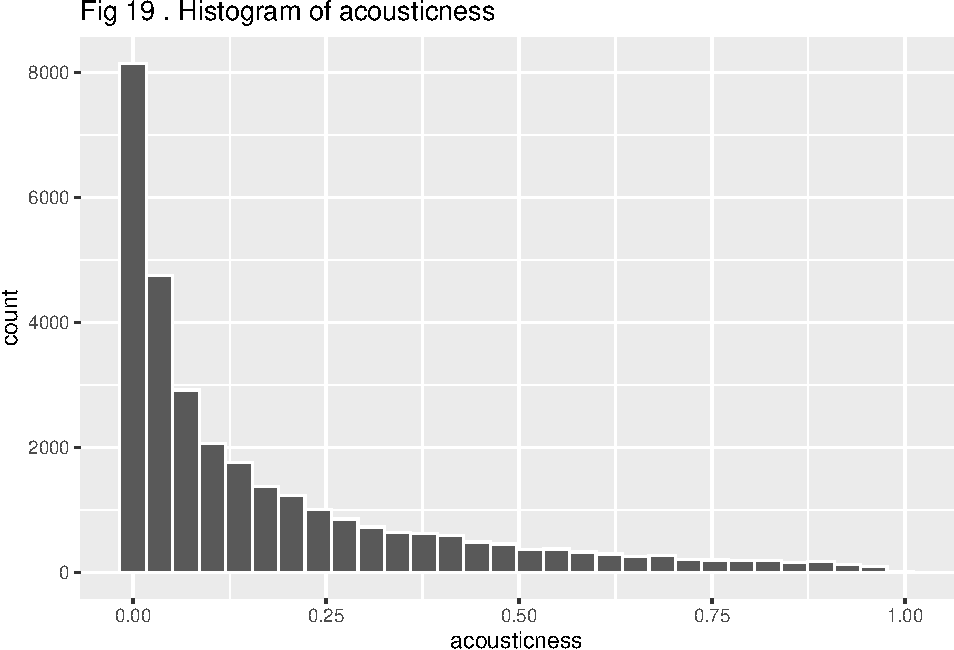
\includegraphics{Final-Report_files/figure-latex/unnamed-chunk-14-15.pdf}

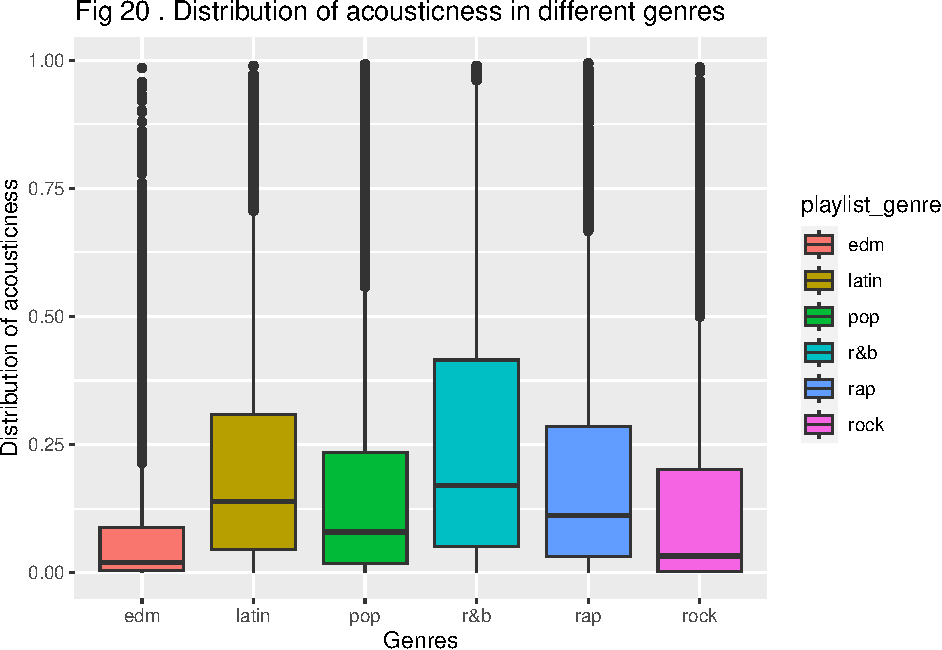
\includegraphics{Final-Report_files/figure-latex/unnamed-chunk-14-16.pdf}

\begin{verbatim}
## 
## acousticness
##       edm     latin       pop       r&b       rap      rock 
## 0.0816723 0.2110486 0.1730262 0.2629757 0.1959889 0.1400041 
##                   Df Sum Sq Mean Sq F value Pr(>F)    
## playlist_genre     5  105.3  21.070     468 <2e-16 ***
## Residuals      30941 1392.9   0.045                   
## ---
## Signif. codes:  0 '***' 0.001 '**' 0.01 '*' 0.05 '.' 0.1 ' ' 1
##   Tukey multiple comparisons of means
##     95% family-wise confidence level
## 
## Fit: aov(formula = as.formula(formula_str), data = spotify_songs)
## 
## $playlist_genre
##                   diff         lwr          upr     p adj
## latin-edm   0.12937634  0.11776115  0.140991532 0.0000000
## pop-edm     0.09135387  0.07994379  0.102763938 0.0000000
## r&b-edm     0.18130339  0.16977004  0.192836749 0.0000000
## rap-edm     0.11431655  0.10299963  0.125633477 0.0000000
## rock-edm    0.05833177  0.04610854  0.070555005 0.0000000
## pop-latin  -0.03802247 -0.04996420 -0.026080746 0.0000000
## r&b-latin   0.05192705  0.03986748  0.063986631 0.0000000
## rap-latin  -0.01505979 -0.02691254 -0.003207029 0.0039839
## rock-latin -0.07104457 -0.08376552 -0.058323620 0.0000000
## r&b-pop     0.08994953  0.07808738  0.101811672 0.0000000
## rap-pop     0.02296269  0.01131087  0.034614509 0.0000003
## rock-pop   -0.03302209 -0.04555603 -0.020488156 0.0000000
## rap-r&b    -0.06698684 -0.07875941 -0.055214266 0.0000000
## rock-r&b   -0.12297162 -0.13561789 -0.110325351 0.0000000
## rock-rap   -0.05598478 -0.06843398 -0.043535581 0.0000000
## 
## [1] "NEXT>>>>NEXT>>>>NEXT>>>>NEXT>>>>NEXT>>>>NEXT>>>>NEXT>>>>"
\end{verbatim}

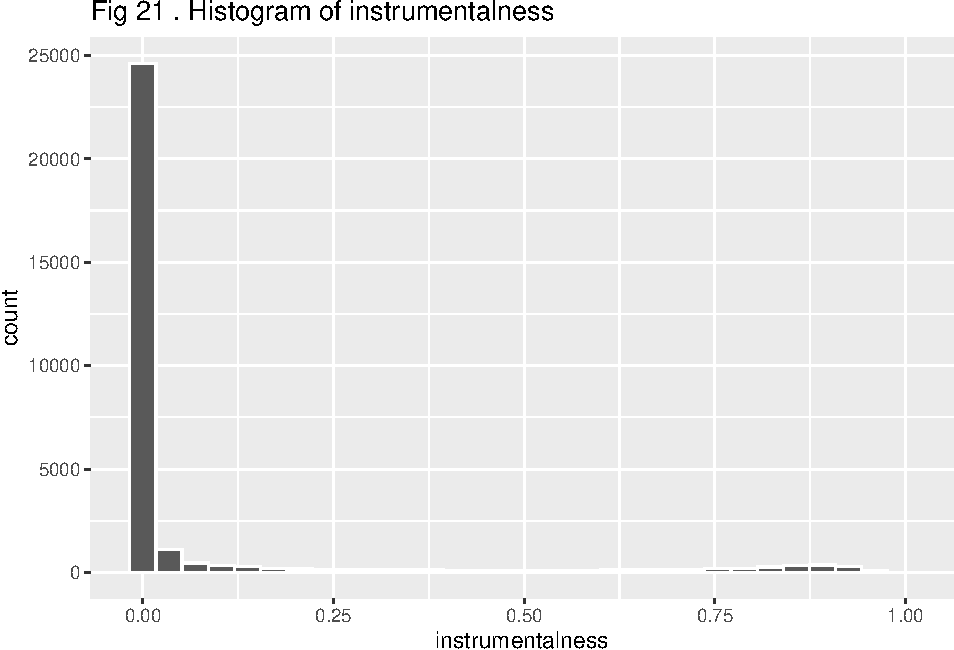
\includegraphics{Final-Report_files/figure-latex/unnamed-chunk-14-17.pdf}

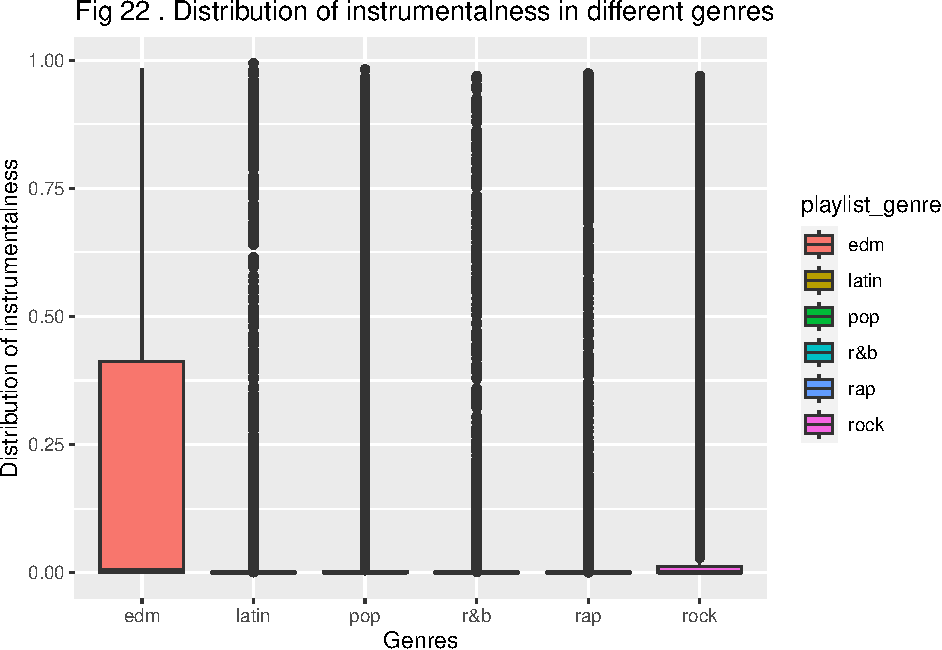
\includegraphics{Final-Report_files/figure-latex/unnamed-chunk-14-18.pdf}

\begin{verbatim}
## 
## instrumentalness
##        edm      latin        pop        r&b        rap       rock 
## 0.21881824 0.04495271 0.05858493 0.02913776 0.07864474 0.06558976 
##                   Df Sum Sq Mean Sq F value Pr(>F)    
## playlist_genre     5  136.1  27.222   575.3 <2e-16 ***
## Residuals      30941 1464.0   0.047                   
## ---
## Signif. codes:  0 '***' 0.001 '**' 0.01 '*' 0.05 '.' 0.1 ' ' 1
##   Tukey multiple comparisons of means
##     95% family-wise confidence level
## 
## Fit: aov(formula = as.formula(formula_str), data = spotify_songs)
## 
## $playlist_genre
##                    diff          lwr           upr     p adj
## latin-edm  -0.173865530 -0.185773460 -0.1619575999 0.0000000
## pop-edm    -0.160233306 -0.171930947 -0.1485356657 0.0000000
## r&b-edm    -0.189680485 -0.201504516 -0.1778564528 0.0000000
## rap-edm    -0.140173500 -0.151775645 -0.1285713561 0.0000000
## rock-edm   -0.153228478 -0.165759774 -0.1406971814 0.0000000
## pop-latin   0.013632224  0.001389527  0.0258749198 0.0188423
## r&b-latin  -0.015814955 -0.028178471 -0.0034514381 0.0036354
## rap-latin   0.033692030  0.021540546  0.0458435136 0.0000000
## rock-latin  0.020637052  0.007595496  0.0336786089 0.0000950
## r&b-pop    -0.029447178 -0.041608286 -0.0172860705 0.0000000
## rap-pop     0.020059806  0.008114323  0.0320052890 0.0000252
## rock-pop    0.007004829 -0.005845004  0.0198546614 0.6293906
## rap-r&b     0.049506984  0.037437706  0.0615762630 0.0000000
## rock-r&b    0.036452007  0.023487011  0.0494170031 0.0000000
## rock-rap   -0.013054977 -0.025817937 -0.0002920174 0.0414948
## 
## [1] "NEXT>>>>NEXT>>>>NEXT>>>>NEXT>>>>NEXT>>>>NEXT>>>>NEXT>>>>"
\end{verbatim}

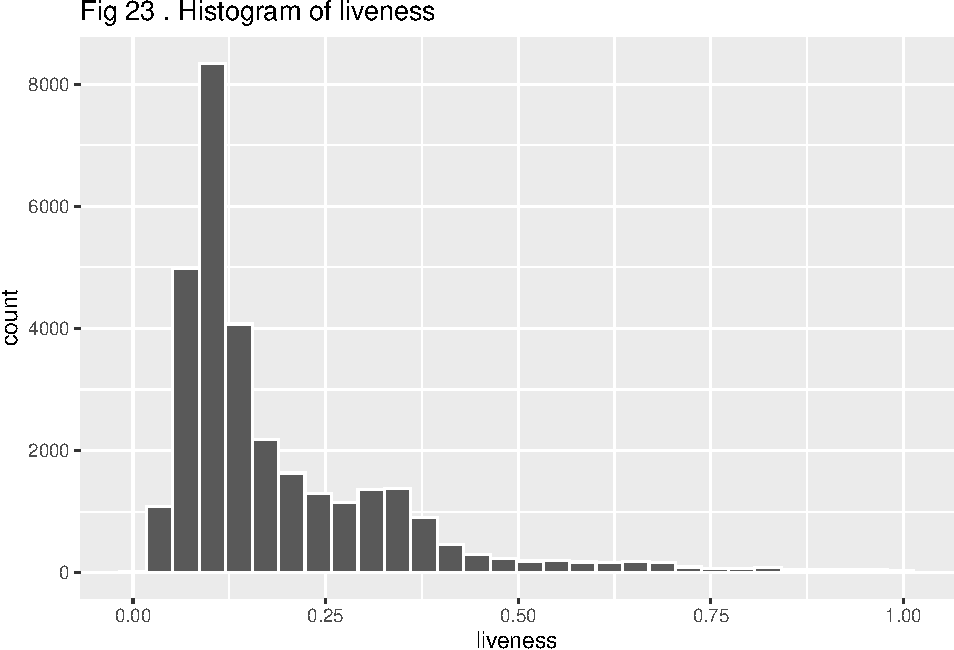
\includegraphics{Final-Report_files/figure-latex/unnamed-chunk-14-19.pdf}

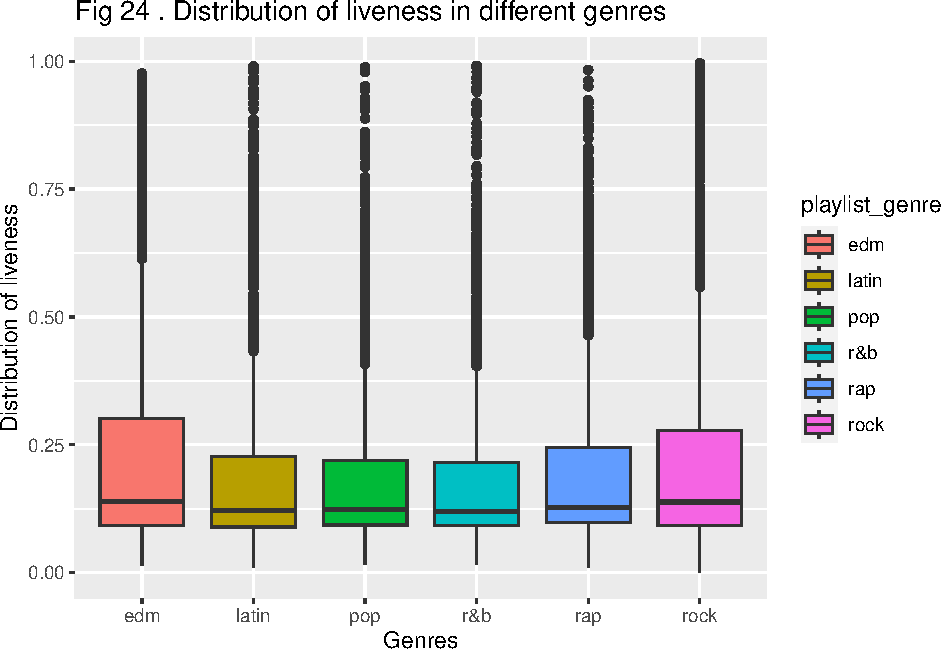
\includegraphics{Final-Report_files/figure-latex/unnamed-chunk-14-20.pdf}

\begin{verbatim}
## 
## liveness
##       edm     latin       pop       r&b       rap      rock 
## 0.2125270 0.1803575 0.1767067 0.1749040 0.1899724 0.2045341 
##                   Df Sum Sq Mean Sq F value Pr(>F)    
## playlist_genre     5    6.5  1.2929   55.04 <2e-16 ***
## Residuals      30941  726.9  0.0235                   
## ---
## Signif. codes:  0 '***' 0.001 '**' 0.01 '*' 0.05 '.' 0.1 ' ' 1
##   Tukey multiple comparisons of means
##     95% family-wise confidence level
## 
## Fit: aov(formula = as.formula(formula_str), data = spotify_songs)
## 
## $playlist_genre
##                    diff          lwr           upr     p adj
## latin-edm  -0.032169489 -0.040559929 -0.0237790481 0.0000000
## pop-edm    -0.035820312 -0.044062580 -0.0275780433 0.0000000
## r&b-edm    -0.037622962 -0.045954287 -0.0292916373 0.0000000
## rap-edm    -0.022554632 -0.030729613 -0.0143796511 0.0000000
## rock-edm   -0.007992933 -0.016822604  0.0008367368 0.1022232
## pop-latin  -0.003650823 -0.012277143  0.0049754965 0.8341357
## r&b-latin  -0.005453474 -0.014164925  0.0032579772 0.4761509
## rap-latin   0.009614857  0.001052806  0.0181769074 0.0172714
## rock-latin  0.024176555  0.014987351  0.0333657595 0.0000000
## r&b-pop    -0.001802650 -0.010371482  0.0067661814 0.9910974
## rap-pop     0.013265680  0.004848780  0.0216825805 0.0001033
## rock-pop    0.027827378  0.018773265  0.0368814923 0.0000000
## rap-r&b     0.015068330  0.006564202  0.0235724586 0.0000066
## rock-r&b    0.029630029  0.020494770  0.0387652880 0.0000000
## rock-rap    0.014561698  0.005568796  0.0235546010 0.0000579
## 
## [1] "NEXT>>>>NEXT>>>>NEXT>>>>NEXT>>>>NEXT>>>>NEXT>>>>NEXT>>>>"
\end{verbatim}

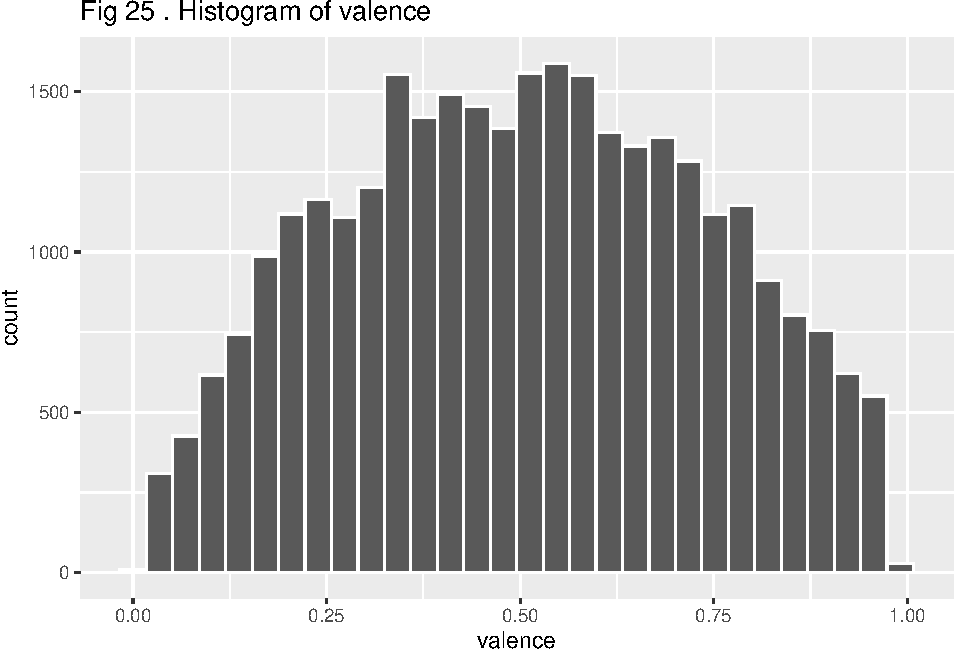
\includegraphics{Final-Report_files/figure-latex/unnamed-chunk-14-21.pdf}

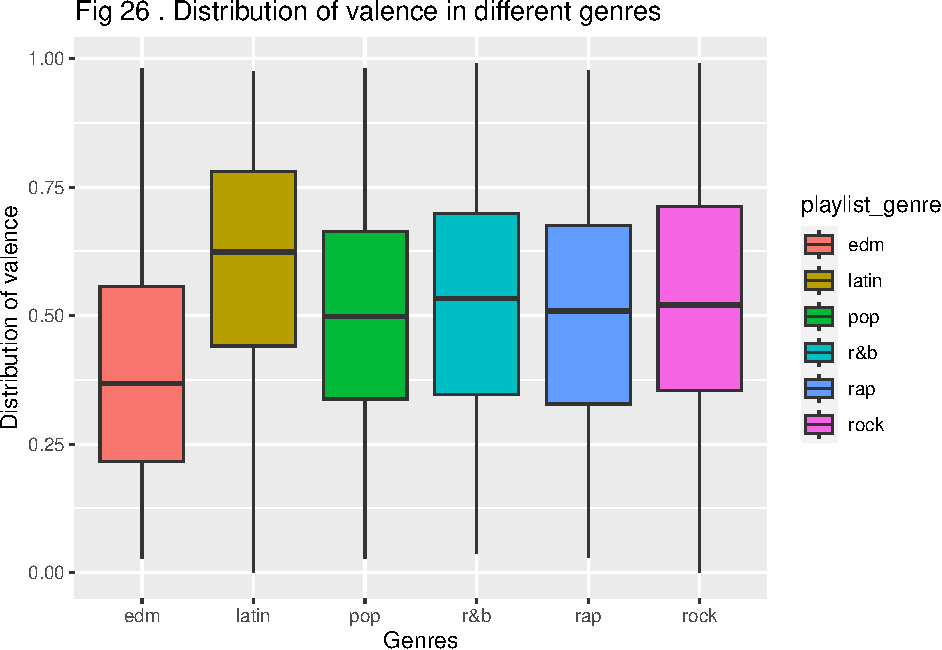
\includegraphics{Final-Report_files/figure-latex/unnamed-chunk-14-22.pdf}

\begin{verbatim}
## 
## valence
##       edm     latin       pop       r&b       rap      rock 
## 0.3984501 0.6027073 0.5004120 0.5236551 0.5000706 0.5311139 
##                   Df Sum Sq Mean Sq F value Pr(>F)    
## playlist_genre     5    120   24.00   477.1 <2e-16 ***
## Residuals      30941   1556    0.05                   
## ---
## Signif. codes:  0 '***' 0.001 '**' 0.01 '*' 0.05 '.' 0.1 ' ' 1
##   Tukey multiple comparisons of means
##     95% family-wise confidence level
## 
## Fit: aov(formula = as.formula(formula_str), data = spotify_songs)
## 
## $playlist_genre
##                     diff          lwr         upr     p adj
## latin-edm   0.2042571750  0.191979625  0.21653472 0.0000000
## pop-edm     0.1019619220  0.089901189  0.11402265 0.0000000
## r&b-edm     0.1252050148  0.113013968  0.13739606 0.0000000
## rap-edm     0.1016204632  0.089658191  0.11358274 0.0000000
## rock-edm    0.1326637807  0.119743516  0.14558405 0.0000000
## pop-latin  -0.1022952530 -0.114917960 -0.08967255 0.0000000
## r&b-latin  -0.0790521602 -0.091799437 -0.06630488 0.0000000
## rap-latin  -0.1026367118 -0.115165375 -0.09010805 0.0000000
## rock-latin -0.0715933943 -0.085039758 -0.05814703 0.0000000
## r&b-pop     0.0232430927  0.010704507  0.03578168 0.0000019
## rap-pop    -0.0003414588 -0.012657727  0.01197481 0.9999996
## rock-pop    0.0307018586  0.017453170  0.04395055 0.0000000
## rap-r&b    -0.0235845516 -0.036028458 -0.01114065 0.0000010
## rock-r&b    0.0074587659 -0.005908661  0.02082619 0.6051412
## rock-rap    0.0310433175  0.017884198  0.04420244 0.0000000
## 
## [1] "NEXT>>>>NEXT>>>>NEXT>>>>NEXT>>>>NEXT>>>>NEXT>>>>NEXT>>>>"
\end{verbatim}

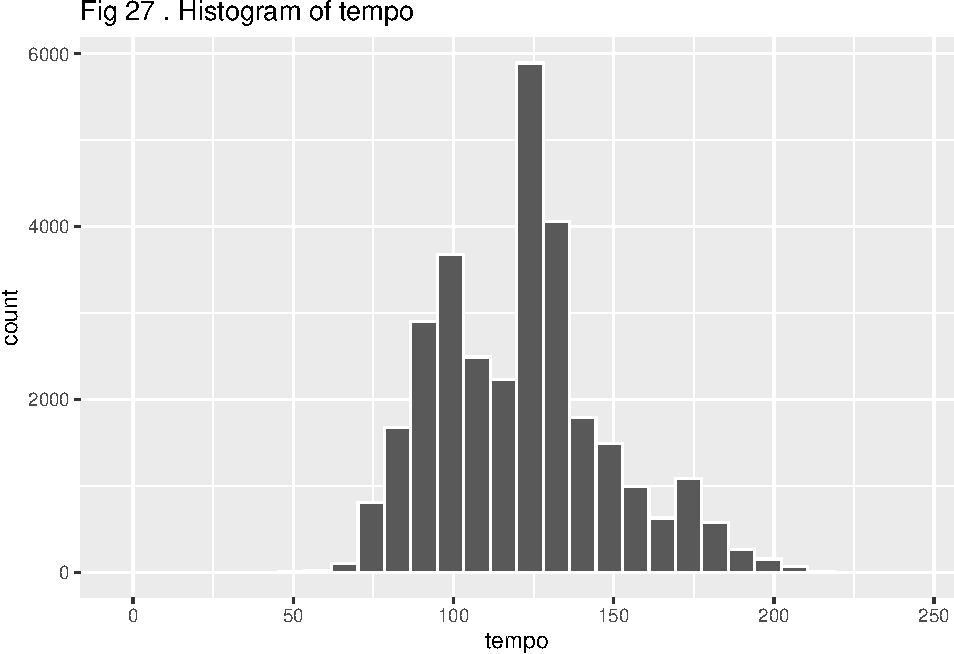
\includegraphics{Final-Report_files/figure-latex/unnamed-chunk-14-23.pdf}

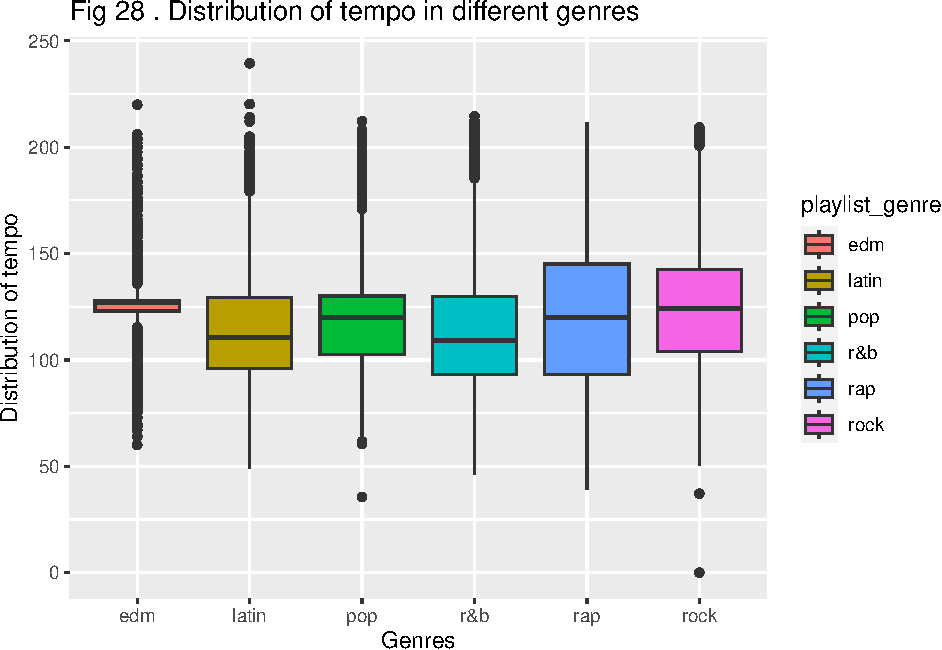
\includegraphics{Final-Report_files/figure-latex/unnamed-chunk-14-24.pdf}

\begin{verbatim}
## 
## tempo
##      edm    latin      pop      r&b      rap     rock 
## 125.7464 118.7115 120.4868 114.2492 121.1452 125.2136 
##                   Df   Sum Sq Mean Sq F value Pr(>F)    
## playlist_genre     5   467636   93527   132.5 <2e-16 ***
## Residuals      30941 21841480     706                   
## ---
## Signif. codes:  0 '***' 0.001 '**' 0.01 '*' 0.05 '.' 0.1 ' ' 1
##   Tukey multiple comparisons of means
##     95% family-wise confidence level
## 
## Fit: aov(formula = as.formula(formula_str), data = spotify_songs)
## 
## $playlist_genre
##                   diff         lwr         upr     p adj
## latin-edm   -7.0348422  -8.4892986  -5.5803857 0.0000000
## pop-edm     -5.2595762  -6.6883475  -3.8308049 0.0000000
## r&b-edm    -11.4971479 -12.9413568 -10.0529390 0.0000000
## rap-edm     -4.6011697  -6.0182768  -3.1840625 0.0000000
## rock-edm    -0.5328016  -2.0633971   0.9977939 0.9206764
## pop-latin    1.7752660   0.2799206   3.2706113 0.0093529
## r&b-latin   -4.4623057  -5.9724083  -2.9522032 0.0000000
## rap-latin    2.4336725   0.9494680   3.9178770 0.0000437
## rock-latin   6.5020406   4.9091209   8.0949602 0.0000000
## r&b-pop     -6.2375717  -7.7229517  -4.7521917 0.0000000
## rap-pop      0.6584065  -0.8006366   2.1174497 0.7929058
## rock-pop     4.7267746   3.1572725   6.2962767 0.0000000
## rap-r&b      6.8959782   5.4218144   8.3701420 0.0000000
## rock-r&b    10.9643463   9.3807779  12.5479147 0.0000000
## rock-rap     4.0683681   2.5094767   5.6272594 0.0000000
## 
## [1] "NEXT>>>>NEXT>>>>NEXT>>>>NEXT>>>>NEXT>>>>NEXT>>>>NEXT>>>>"
\end{verbatim}

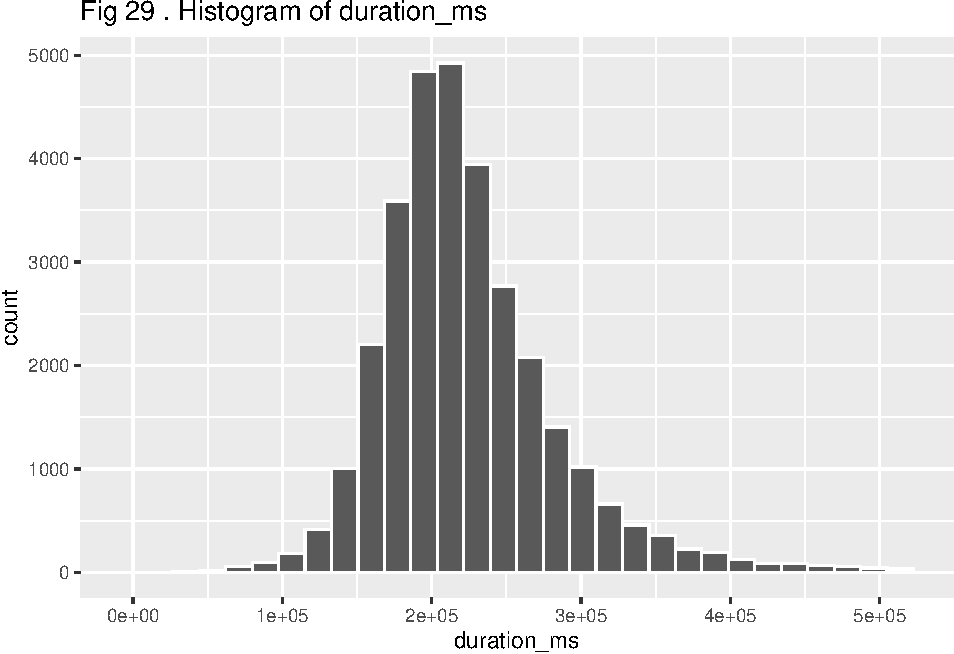
\includegraphics{Final-Report_files/figure-latex/unnamed-chunk-14-25.pdf}

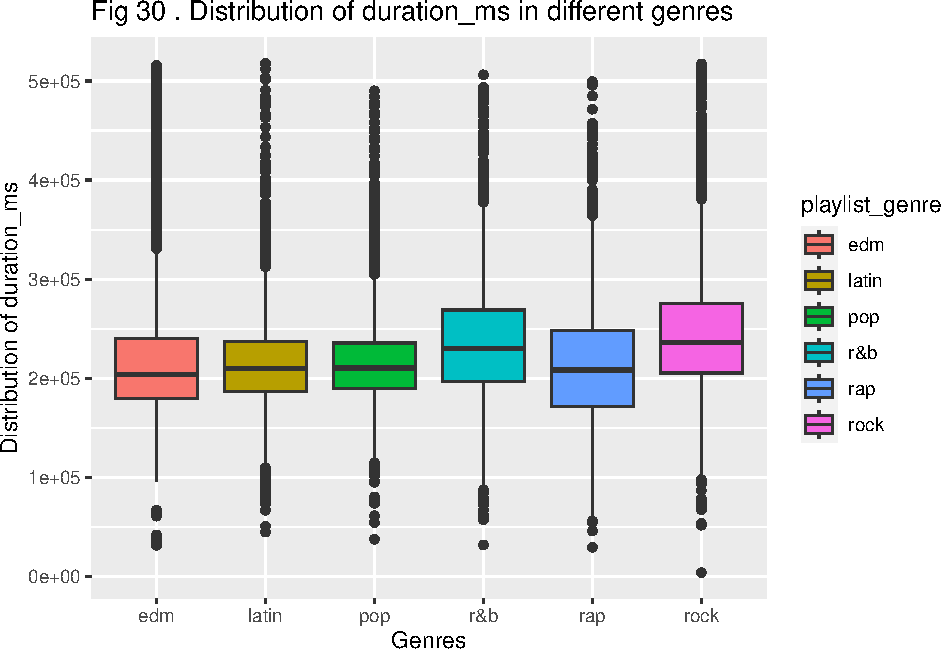
\includegraphics{Final-Report_files/figure-latex/unnamed-chunk-14-26.pdf}

\begin{verbatim}
## 
## duration_ms
##      edm    latin      pop      r&b      rap     rock 
## 221647.9 215760.6 216827.5 236093.9 211773.5 247319.9 
##                   Df    Sum Sq   Mean Sq F value Pr(>F)    
## playlist_genre     5 4.461e+12 8.922e+11   266.2 <2e-16 ***
## Residuals      30941 1.037e+14 3.351e+09                   
## ---
## Signif. codes:  0 '***' 0.001 '**' 0.01 '*' 0.05 '.' 0.1 ' ' 1
##   Tukey multiple comparisons of means
##     95% family-wise confidence level
## 
## Fit: aov(formula = as.formula(formula_str), data = spotify_songs)
## 
## $playlist_genre
##                  diff        lwr        upr     p adj
## latin-edm   -5887.289  -9056.156  -2718.422 0.0000018
## pop-edm     -4820.402  -7933.309  -1707.496 0.0001484
## r&b-edm     14445.948  11299.407  17592.489 0.0000000
## rap-edm     -9874.436 -12961.930  -6786.943 0.0000000
## rock-edm    25671.992  22337.238  29006.746 0.0000000
## pop-latin    1066.887  -2191.067   4324.840 0.9380135
## r&b-latin   20333.237  17043.131  23623.342 0.0000000
## rap-latin   -3987.148  -7220.828   -753.467 0.0058983
## rock-latin  31559.281  28088.740  35029.823 0.0000000
## r&b-pop     19266.350  16030.108  22502.591 0.0000000
## rap-pop     -5054.034  -8232.895  -1875.174 0.0000860
## rock-pop    30492.394  27072.874  33911.915 0.0000000
## rap-r&b    -24320.384 -27532.189 -21108.580 0.0000000
## rock-r&b    11226.045   7775.877  14676.212 0.0000000
## rock-rap    35546.429  32150.026  38942.832 0.0000000
## 
## [1] "NEXT>>>>NEXT>>>>NEXT>>>>NEXT>>>>NEXT>>>>NEXT>>>>NEXT>>>>"
\end{verbatim}

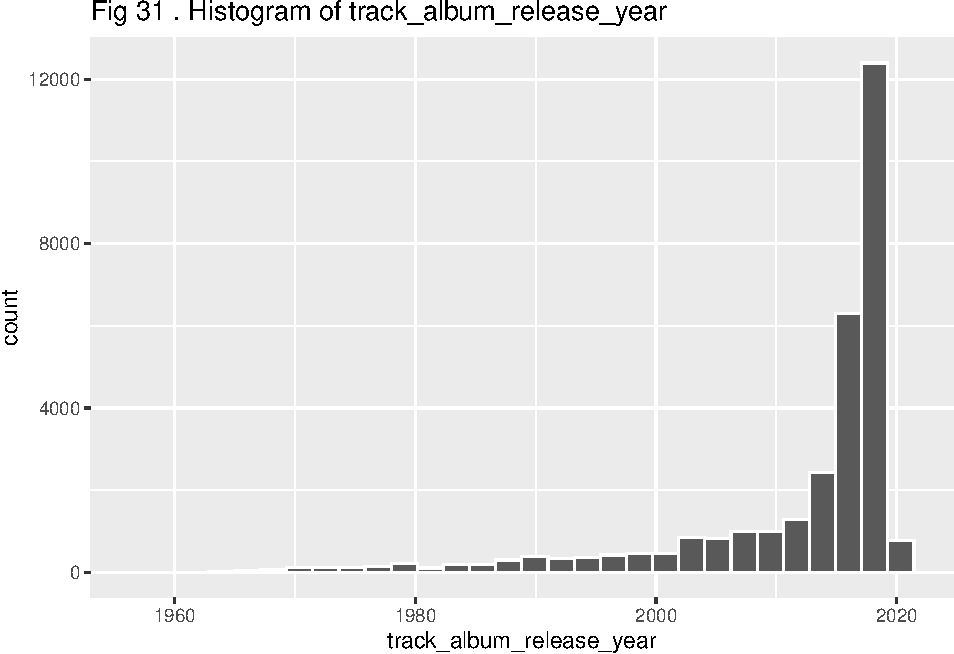
\includegraphics{Final-Report_files/figure-latex/unnamed-chunk-14-27.pdf}

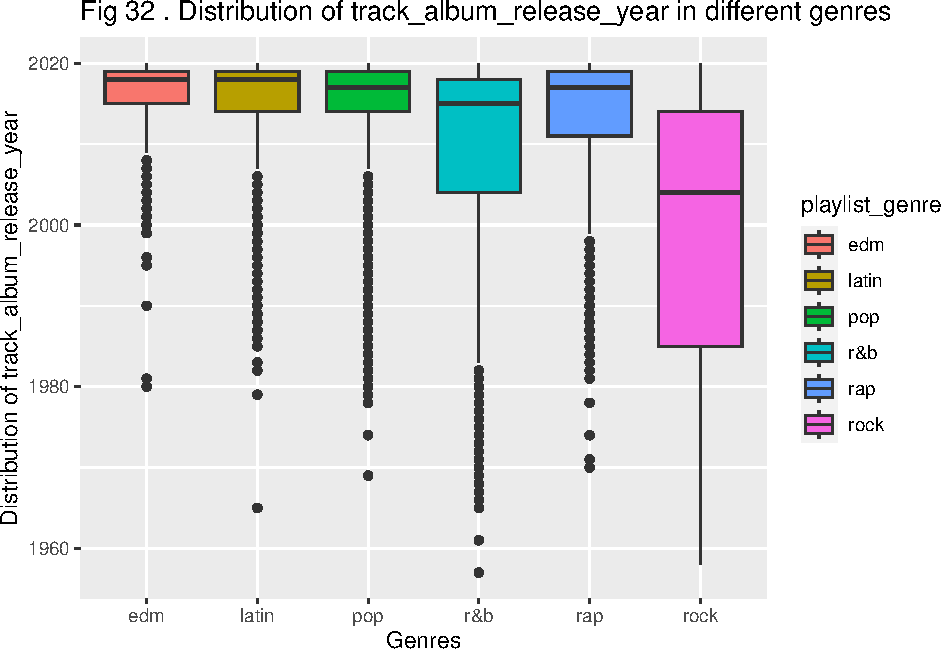
\includegraphics{Final-Report_files/figure-latex/unnamed-chunk-14-28.pdf}

\begin{verbatim}
## 
## track_album_release_year
##      edm    latin      pop      r&b      rap     rock 
## 2016.780 2015.176 2014.843 2010.361 2013.411 1999.331 
##                   Df  Sum Sq Mean Sq F value Pr(>F)    
## playlist_genre     5  918246  183649    2341 <2e-16 ***
## Residuals      30941 2427434      78                   
## ---
## Signif. codes:  0 '***' 0.001 '**' 0.01 '*' 0.05 '.' 0.1 ' ' 1
##   Tukey multiple comparisons of means
##     95% family-wise confidence level
## 
## Fit: aov(formula = as.formula(formula_str), data = spotify_songs)
## 
## $playlist_genre
##                   diff         lwr         upr     p adj
## latin-edm   -1.6037595  -2.0886385  -1.1188805 0.0000000
## pop-edm     -1.9365664  -2.4128826  -1.4602501 0.0000000
## r&b-edm     -6.4188497  -6.9003124  -5.9373869 0.0000000
## rap-edm     -3.3686033  -3.8410310  -2.8961755 0.0000000
## rock-edm   -17.4487799 -17.9590418 -16.9385181 0.0000000
## pop-latin   -0.3328069  -0.8313173   0.1657034 0.4005061
## r&b-latin   -4.8150902  -5.3185202  -4.3116602 0.0000000
## rap-latin   -1.7648438  -2.2596401  -1.2700475 0.0000000
## rock-latin -15.8450205 -16.3760596 -15.3139813 0.0000000
## r&b-pop     -4.4822833  -4.9774714  -3.9870952 0.0000000
## rap-pop     -1.4320369  -1.9184450  -0.9456288 0.0000000
## rock-pop   -15.5122135 -16.0354459 -14.9889812 0.0000000
## rap-r&b      3.0502464   2.5587975   3.5416954 0.0000000
## rock-r&b   -11.0299302 -11.5578519 -10.5020086 0.0000000
## rock-rap   -14.0801767 -14.5998716 -13.5604817 0.0000000
## 
## [1] "NEXT>>>>NEXT>>>>NEXT>>>>NEXT>>>>NEXT>>>>NEXT>>>>NEXT>>>>"
\end{verbatim}

How does track popularity change over time

\begin{Shaded}
\begin{Highlighting}[]
\NormalTok{spotify\_songs }\OtherTok{\textless{}{-}}\NormalTok{ spotify\_songs }\SpecialCharTok{\%\textgreater{}\%}
  \FunctionTok{mutate}\NormalTok{(}\AttributeTok{year\_group =} \DecValTok{5} \SpecialCharTok{*}\NormalTok{ (track\_album\_release\_year }\SpecialCharTok{\%/\%} \DecValTok{5}\NormalTok{))}

\NormalTok{spotify\_songs }\SpecialCharTok{\%\textgreater{}\%}
  \FunctionTok{ggplot}\NormalTok{(}\FunctionTok{aes}\NormalTok{(}\AttributeTok{x =} \FunctionTok{factor}\NormalTok{(year\_group), }
             \AttributeTok{y =}\NormalTok{ track\_popularity,}
             \AttributeTok{fill =}\NormalTok{ year\_group)) }\SpecialCharTok{+}
  \FunctionTok{geom\_boxplot}\NormalTok{() }\SpecialCharTok{+}
  \FunctionTok{xlab}\NormalTok{(}\StringTok{"Year Group (5{-}year intervals)"}\NormalTok{) }\SpecialCharTok{+}
  \FunctionTok{ylab}\NormalTok{(}\StringTok{"Track Popularity"}\NormalTok{) }\SpecialCharTok{+}
  \FunctionTok{ggtitle}\NormalTok{(}\StringTok{"Fig33. Track Popularity by 5{-}year Intervals"}\NormalTok{) }\SpecialCharTok{+}
  \FunctionTok{theme\_minimal}\NormalTok{()}
\end{Highlighting}
\end{Shaded}

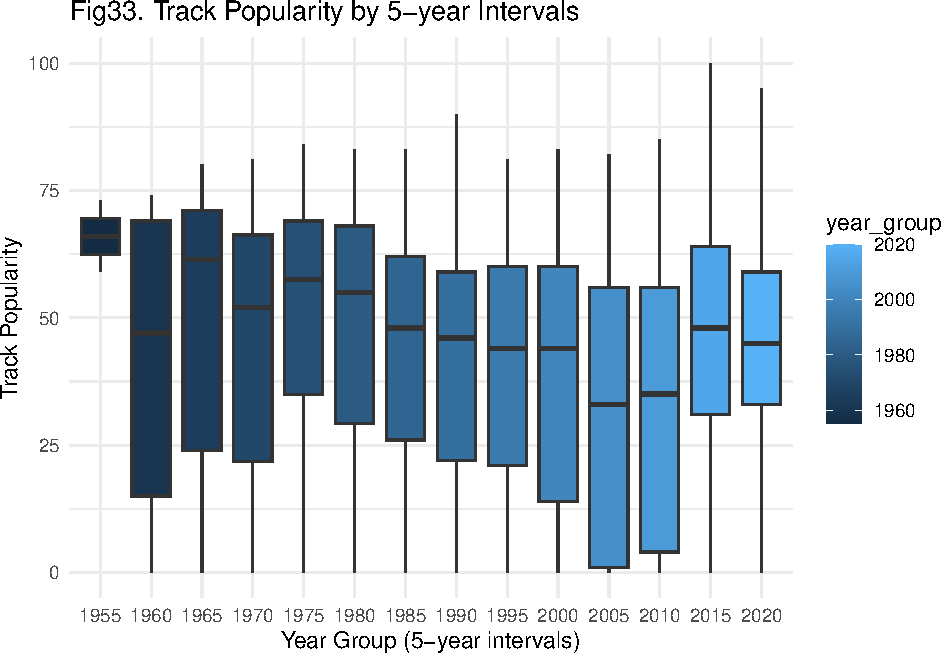
\includegraphics{Final-Report_files/figure-latex/unnamed-chunk-15-1.pdf}

\begin{Shaded}
\begin{Highlighting}[]
\NormalTok{spotify\_songs }\OtherTok{\textless{}{-}}\NormalTok{ spotify\_songs }\SpecialCharTok{\%\textgreater{}\%} 
\NormalTok{  dplyr}\SpecialCharTok{::}\FunctionTok{select}\NormalTok{(}\SpecialCharTok{{-}}\NormalTok{year\_group)}
\end{Highlighting}
\end{Shaded}

\begin{Shaded}
\begin{Highlighting}[]
\NormalTok{spotify\_songs }\SpecialCharTok{\%\textgreater{}\%}
  \FunctionTok{group\_by}\NormalTok{(track\_album\_release\_year) }\SpecialCharTok{\%\textgreater{}\%}
  \FunctionTok{summarize}\NormalTok{(}\AttributeTok{avg\_popularity =} \FunctionTok{mean}\NormalTok{(track\_popularity)) }\SpecialCharTok{\%\textgreater{}\%}
  \FunctionTok{ggplot}\NormalTok{(}\FunctionTok{aes}\NormalTok{(}\AttributeTok{x =}\NormalTok{ track\_album\_release\_year, }\AttributeTok{y =}\NormalTok{ avg\_popularity)) }\SpecialCharTok{+}
  \FunctionTok{geom\_point}\NormalTok{() }\SpecialCharTok{+}
  \FunctionTok{geom\_line}\NormalTok{() }\SpecialCharTok{+}
  \FunctionTok{xlab}\NormalTok{(}\StringTok{"Year"}\NormalTok{) }\SpecialCharTok{+}
  \FunctionTok{ylab}\NormalTok{(}\StringTok{"Average Track Popularity"}\NormalTok{) }\SpecialCharTok{+}
  \FunctionTok{ggtitle}\NormalTok{(}\StringTok{"Fig34. Average Track Popularity by Year"}\NormalTok{) }\SpecialCharTok{+}
  \FunctionTok{theme\_minimal}\NormalTok{()}
\end{Highlighting}
\end{Shaded}

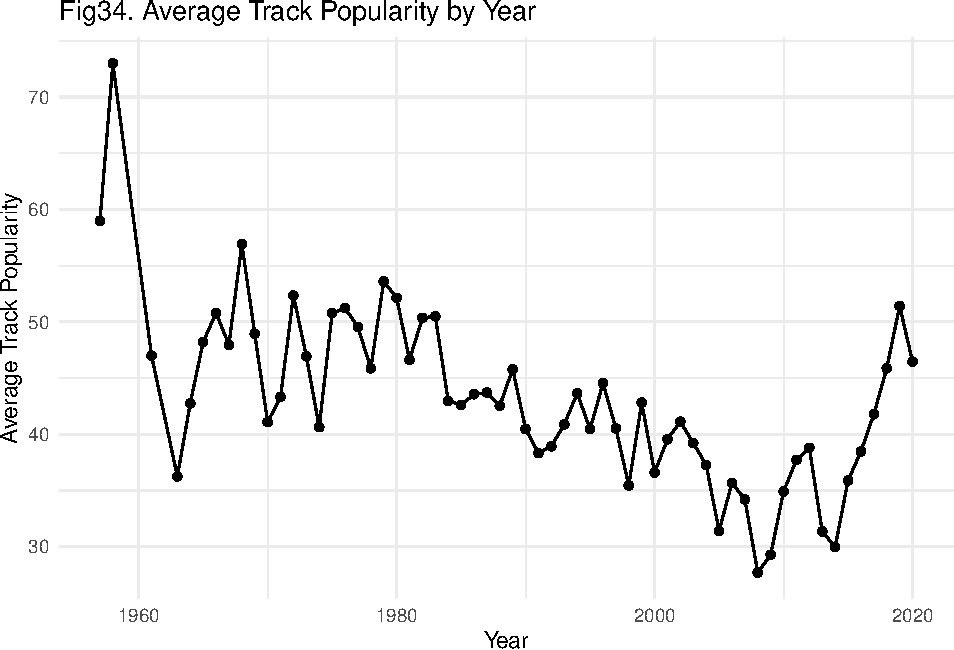
\includegraphics{Final-Report_files/figure-latex/unnamed-chunk-16-1.pdf}

\begin{Shaded}
\begin{Highlighting}[]
\NormalTok{spotify\_songs }\SpecialCharTok{\%\textgreater{}\%} \FunctionTok{ggplot}\NormalTok{(}\FunctionTok{aes}\NormalTok{(}\AttributeTok{x =}\NormalTok{ track\_album\_release\_year, }\AttributeTok{y =}\NormalTok{track\_popularity)) }\SpecialCharTok{+}
  \FunctionTok{geom\_point}\NormalTok{(}\AttributeTok{alpha =} \FloatTok{0.1}\NormalTok{) }\SpecialCharTok{+}
  \FunctionTok{geom\_smooth}\NormalTok{( }\AttributeTok{formula =}\NormalTok{ y }\SpecialCharTok{\textasciitilde{}}\NormalTok{ x, }\AttributeTok{method =} \StringTok{"loess"}\NormalTok{) }\SpecialCharTok{+}
  \FunctionTok{ggtitle}\NormalTok{(}\StringTok{"Fig3.Track\_popularity{-}Year(detaied)"}\NormalTok{) }
\end{Highlighting}
\end{Shaded}

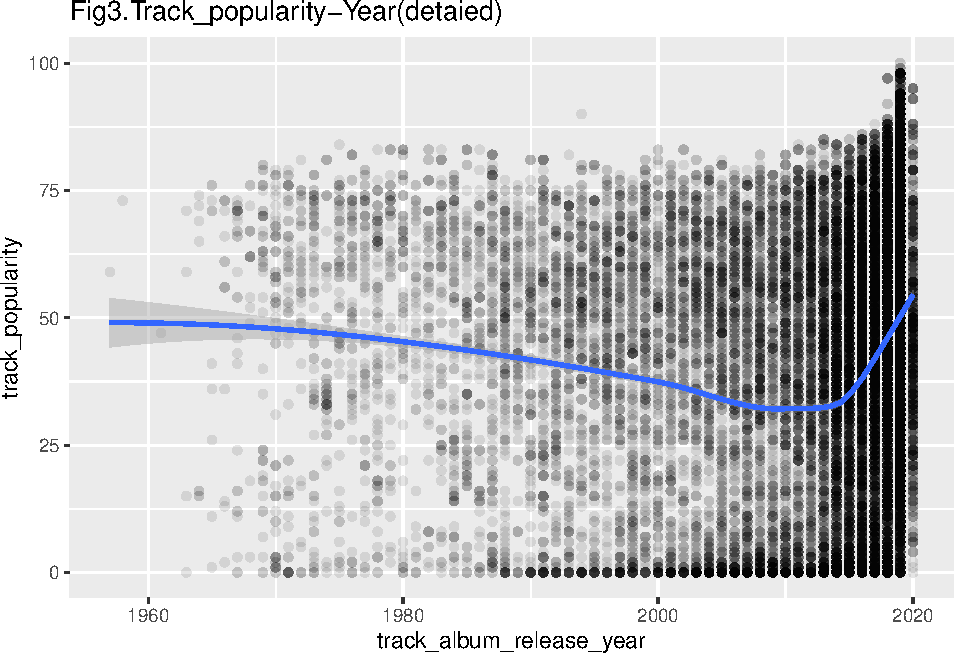
\includegraphics{Final-Report_files/figure-latex/unnamed-chunk-17-1.pdf}

\begin{Shaded}
\begin{Highlighting}[]
\NormalTok{linear\_model }\OtherTok{\textless{}{-}} \FunctionTok{lm}\NormalTok{(track\_popularity }\SpecialCharTok{\textasciitilde{}}\NormalTok{track\_album\_release\_year, }
                   \AttributeTok{data =}\NormalTok{ spotify\_songs)}

\FunctionTok{summary}\NormalTok{(linear\_model)}
\end{Highlighting}
\end{Shaded}

\begin{verbatim}
## 
## Call:
## lm(formula = track_popularity ~ track_album_release_year, data = spotify_songs)
## 
## Residuals:
##     Min      1Q  Median      3Q     Max 
## -43.998 -18.037   2.524  19.364  56.162 
## 
## Coefficients:
##                            Estimate Std. Error t value Pr(>|t|)    
## (Intercept)              -279.38805   27.39308  -10.20   <2e-16 ***
## track_album_release_year    0.16009    0.01361   11.76   <2e-16 ***
## ---
## Signif. codes:  0 '***' 0.001 '**' 0.01 '*' 0.05 '.' 0.1 ' ' 1
## 
## Residual standard error: 24.9 on 30945 degrees of freedom
## Multiple R-squared:  0.004449,   Adjusted R-squared:  0.004417 
## F-statistic: 138.3 on 1 and 30945 DF,  p-value: < 2.2e-16
\end{verbatim}

\textbf{PCA}

\begin{Shaded}
\begin{Highlighting}[]
\NormalTok{spotify\_songs\_recipe\_PCA }\OtherTok{\textless{}{-}} \FunctionTok{recipe}\NormalTok{( playlist\_genre }\SpecialCharTok{\textasciitilde{}}\NormalTok{ ., }\AttributeTok{data =}\NormalTok{ spotify\_songs ) }\SpecialCharTok{\%\textgreater{}\%} 
  \FunctionTok{step\_normalize}\NormalTok{(}\FunctionTok{all\_predictors}\NormalTok{() ) }\SpecialCharTok{\%\textgreater{}\%} \CommentTok{\# Normalise our predictors }
  \FunctionTok{step\_pca}\NormalTok{(}\FunctionTok{all\_predictors}\NormalTok{() ) }\CommentTok{\# Do the PCA.}
\NormalTok{spotify\_songs\_recipe\_PCA}
\end{Highlighting}
\end{Shaded}

\begin{verbatim}
## 
\end{verbatim}

\begin{verbatim}
## -- Recipe ----------------------------------------------------------------------
\end{verbatim}

\begin{verbatim}
## 
\end{verbatim}

\begin{verbatim}
## -- Inputs
\end{verbatim}

\begin{verbatim}
## Number of variables by role
\end{verbatim}

\begin{verbatim}
## outcome:    1
## predictor: 14
\end{verbatim}

\begin{verbatim}
## 
\end{verbatim}

\begin{verbatim}
## -- Operations
\end{verbatim}

\begin{verbatim}
## * Centering and scaling for: all_predictors()
\end{verbatim}

\begin{verbatim}
## * PCA extraction with: all_predictors()
\end{verbatim}

\begin{Shaded}
\begin{Highlighting}[]
\NormalTok{spotify\_songs\_prepped }\OtherTok{\textless{}{-}}\NormalTok{ spotify\_songs\_recipe\_PCA }\SpecialCharTok{\%\textgreater{}\%} \FunctionTok{prep}\NormalTok{() }
\FunctionTok{tidy}\NormalTok{(spotify\_songs\_prepped)}
\end{Highlighting}
\end{Shaded}

\begin{verbatim}
## # A tibble: 2 x 6
##   number operation type      trained skip  id             
##    <int> <chr>     <chr>     <lgl>   <lgl> <chr>          
## 1      1 step      normalize TRUE    FALSE normalize_LQOKm
## 2      2 step      pca       TRUE    FALSE pca_3KvVU
\end{verbatim}

\begin{Shaded}
\begin{Highlighting}[]
\NormalTok{sdev }\OtherTok{\textless{}{-}}\NormalTok{ spotify\_songs\_prepped}\SpecialCharTok{$}\NormalTok{steps[[}\DecValTok{2}\NormalTok{]]}\SpecialCharTok{$}\NormalTok{res}\SpecialCharTok{$}\NormalTok{sdev}
\NormalTok{ve }\OtherTok{\textless{}{-}}\NormalTok{ sdev}\SpecialCharTok{\^{}}\DecValTok{2} \SpecialCharTok{/} \FunctionTok{sum}\NormalTok{(sdev }\SpecialCharTok{\^{}}\DecValTok{2}\NormalTok{)}

\NormalTok{variance\_explained }\OtherTok{\textless{}{-}}\NormalTok{ ve }\SpecialCharTok{*} \DecValTok{100}

\NormalTok{sorted\_var\_explained }\OtherTok{\textless{}{-}} \FunctionTok{sort}\NormalTok{(variance\_explained, }\AttributeTok{decreasing =} \ConstantTok{TRUE}\NormalTok{)}

\NormalTok{cumulative\_var\_explained }\OtherTok{\textless{}{-}} \FunctionTok{cumsum}\NormalTok{(sorted\_var\_explained)}
\NormalTok{PC\_CUM }\OtherTok{\textless{}{-}} \FunctionTok{data.frame}\NormalTok{(}\AttributeTok{PC =} \DecValTok{1}\SpecialCharTok{:}\FunctionTok{length}\NormalTok{(cumulative\_var\_explained), }
                     \AttributeTok{cumulative\_var\_explained =}\NormalTok{ cumulative\_var\_explained)}
\NormalTok{PC\_CUM }\SpecialCharTok{\%\textgreater{}\%} \FunctionTok{filter}\NormalTok{(cumulative\_var\_explained }\SpecialCharTok{\textgreater{}} \DecValTok{95}\NormalTok{)}
\end{Highlighting}
\end{Shaded}

\begin{verbatim}
##   PC cumulative_var_explained
## 1 12                 95.56142
## 2 13                 98.48400
## 3 14                100.00000
\end{verbatim}

\begin{Shaded}
\begin{Highlighting}[]
\NormalTok{PC\_CUM }\SpecialCharTok{\%\textgreater{}\%} \FunctionTok{ggplot}\NormalTok{(}\FunctionTok{aes}\NormalTok{(}\AttributeTok{x =}\NormalTok{ PC , }\AttributeTok{y =}\NormalTok{ cumulative\_var\_explained)) }\SpecialCharTok{+} \FunctionTok{geom\_point}\NormalTok{() }\SpecialCharTok{+} \FunctionTok{geom\_line}\NormalTok{() }\SpecialCharTok{+}
  \FunctionTok{ggtitle}\NormalTok{(}\StringTok{"Fig36. Proportion of Total Variance Explained by PC"}\NormalTok{) }\SpecialCharTok{+} \FunctionTok{xlab}\NormalTok{(}\StringTok{"PC"}\NormalTok{) }\SpecialCharTok{+}
  \FunctionTok{ylab}\NormalTok{(}\StringTok{"Proportion of Variance Explained"}\NormalTok{)}
\end{Highlighting}
\end{Shaded}

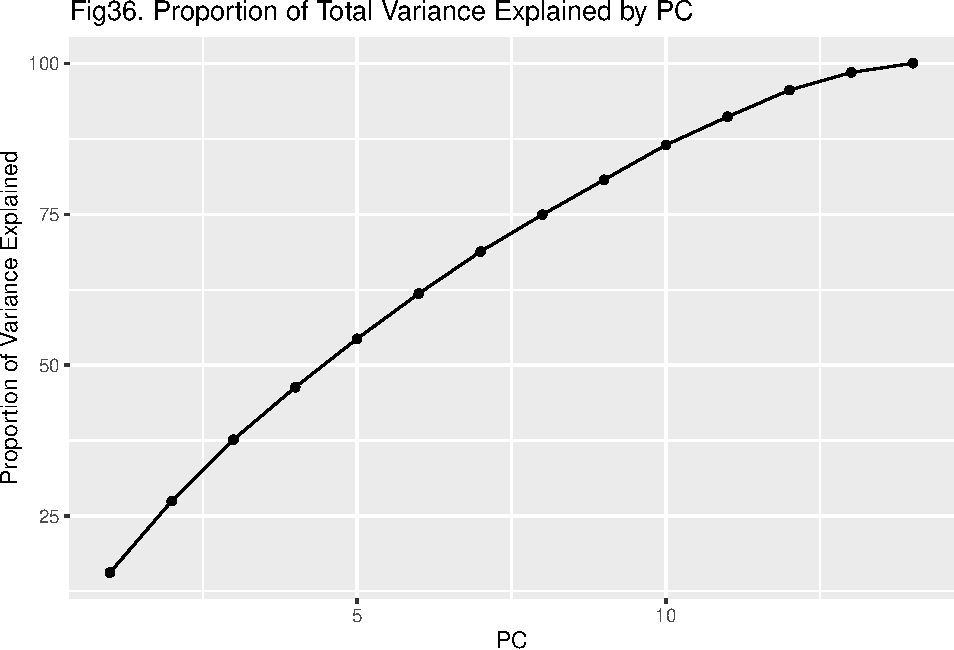
\includegraphics{Final-Report_files/figure-latex/unnamed-chunk-20-1.pdf}

\hypertarget{modeling}{%
\subsection{1.4 Modeling}\label{modeling}}

\hypertarget{sampling-to-reduce-data-set-size}{%
\subsubsection{Sampling to reduce data set
size}\label{sampling-to-reduce-data-set-size}}

\begin{Shaded}
\begin{Highlighting}[]
\FunctionTok{set.seed}\NormalTok{(}\DecValTok{1897402}\NormalTok{)}
\NormalTok{songs\_per\_genre }\OtherTok{\textless{}{-}} \DecValTok{1000}

\NormalTok{spotify\_songs\_sampled  }\OtherTok{\textless{}{-}}\NormalTok{ spotify\_songs }\SpecialCharTok{\%\textgreater{}\%}
  \FunctionTok{group\_by}\NormalTok{(playlist\_genre) }\SpecialCharTok{\%\textgreater{}\%}
  \FunctionTok{sample\_n}\NormalTok{(songs\_per\_genre) }\SpecialCharTok{\%\textgreater{}\%}
  \FunctionTok{ungroup}\NormalTok{()}

\FunctionTok{skim}\NormalTok{(spotify\_songs\_sampled)}
\end{Highlighting}
\end{Shaded}

\begin{longtable}[]{@{}ll@{}}
\caption{Data summary}\tabularnewline
\toprule()
\endhead
Name & spotify\_songs\_sampled \\
Number of rows & 6000 \\
Number of columns & 15 \\
\_\_\_\_\_\_\_\_\_\_\_\_\_\_\_\_\_\_\_\_\_\_\_ & \\
Column type frequency: & \\
factor & 1 \\
numeric & 14 \\
\_\_\_\_\_\_\_\_\_\_\_\_\_\_\_\_\_\_\_\_\_\_\_\_ & \\
Group variables & None \\
\bottomrule()
\end{longtable}

\textbf{Variable type: factor}

\begin{longtable}[]{@{}
  >{\raggedright\arraybackslash}p{(\columnwidth - 10\tabcolsep) * \real{0.1515}}
  >{\raggedleft\arraybackslash}p{(\columnwidth - 10\tabcolsep) * \real{0.1010}}
  >{\raggedleft\arraybackslash}p{(\columnwidth - 10\tabcolsep) * \real{0.1414}}
  >{\raggedright\arraybackslash}p{(\columnwidth - 10\tabcolsep) * \real{0.0808}}
  >{\raggedleft\arraybackslash}p{(\columnwidth - 10\tabcolsep) * \real{0.0909}}
  >{\raggedright\arraybackslash}p{(\columnwidth - 10\tabcolsep) * \real{0.4343}}@{}}
\toprule()
\begin{minipage}[b]{\linewidth}\raggedright
skim\_variable
\end{minipage} & \begin{minipage}[b]{\linewidth}\raggedleft
n\_missing
\end{minipage} & \begin{minipage}[b]{\linewidth}\raggedleft
complete\_rate
\end{minipage} & \begin{minipage}[b]{\linewidth}\raggedright
ordered
\end{minipage} & \begin{minipage}[b]{\linewidth}\raggedleft
n\_unique
\end{minipage} & \begin{minipage}[b]{\linewidth}\raggedright
top\_counts
\end{minipage} \\
\midrule()
\endhead
playlist\_genre & 0 & 1 & FALSE & 6 & edm: 1000, lat: 1000, pop: 1000,
r\&b: 1000 \\
\bottomrule()
\end{longtable}

\textbf{Variable type: numeric}

\begin{longtable}[]{@{}
  >{\raggedright\arraybackslash}p{(\columnwidth - 20\tabcolsep) * \real{0.2033}}
  >{\raggedleft\arraybackslash}p{(\columnwidth - 20\tabcolsep) * \real{0.0813}}
  >{\raggedleft\arraybackslash}p{(\columnwidth - 20\tabcolsep) * \real{0.1138}}
  >{\raggedleft\arraybackslash}p{(\columnwidth - 20\tabcolsep) * \real{0.0813}}
  >{\raggedleft\arraybackslash}p{(\columnwidth - 20\tabcolsep) * \real{0.0732}}
  >{\raggedleft\arraybackslash}p{(\columnwidth - 20\tabcolsep) * \real{0.0732}}
  >{\raggedleft\arraybackslash}p{(\columnwidth - 20\tabcolsep) * \real{0.0813}}
  >{\raggedleft\arraybackslash}p{(\columnwidth - 20\tabcolsep) * \real{0.0813}}
  >{\raggedleft\arraybackslash}p{(\columnwidth - 20\tabcolsep) * \real{0.0813}}
  >{\raggedleft\arraybackslash}p{(\columnwidth - 20\tabcolsep) * \real{0.0813}}
  >{\raggedright\arraybackslash}p{(\columnwidth - 20\tabcolsep) * \real{0.0488}}@{}}
\toprule()
\begin{minipage}[b]{\linewidth}\raggedright
skim\_variable
\end{minipage} & \begin{minipage}[b]{\linewidth}\raggedleft
n\_missing
\end{minipage} & \begin{minipage}[b]{\linewidth}\raggedleft
complete\_rate
\end{minipage} & \begin{minipage}[b]{\linewidth}\raggedleft
mean
\end{minipage} & \begin{minipage}[b]{\linewidth}\raggedleft
sd
\end{minipage} & \begin{minipage}[b]{\linewidth}\raggedleft
p0
\end{minipage} & \begin{minipage}[b]{\linewidth}\raggedleft
p25
\end{minipage} & \begin{minipage}[b]{\linewidth}\raggedleft
p50
\end{minipage} & \begin{minipage}[b]{\linewidth}\raggedleft
p75
\end{minipage} & \begin{minipage}[b]{\linewidth}\raggedleft
p100
\end{minipage} & \begin{minipage}[b]{\linewidth}\raggedright
hist
\end{minipage} \\
\midrule()
\endhead
track\_popularity & 0 & 1 & 42.77 & 24.69 & 0.00 & 25.00 & 46.00 & 62.00
& 98.00 & ▆▆▇▇▂ \\
danceability & 0 & 1 & 0.65 & 0.15 & 0.08 & 0.56 & 0.67 & 0.76 & 0.97 &
▁▂▅▇▃ \\
energy & 0 & 1 & 0.70 & 0.18 & 0.02 & 0.58 & 0.72 & 0.84 & 1.00 &
▁▁▅▇▇ \\
key & 0 & 1 & 5.42 & 3.63 & 0.00 & 2.00 & 6.00 & 9.00 & 11.00 & ▇▂▅▅▇ \\
loudness & 0 & 1 & -6.70 & 3.02 & -36.51 & -8.17 & -6.14 & -4.60 & 0.64
& ▁▁▁▅▇ \\
mode & 0 & 1 & 0.56 & 0.50 & 0.00 & 0.00 & 1.00 & 1.00 & 1.00 & ▆▁▁▁▇ \\
speechiness & 0 & 1 & 0.11 & 0.10 & 0.02 & 0.04 & 0.06 & 0.13 & 0.86 &
▇▁▁▁▁ \\
acousticness & 0 & 1 & 0.18 & 0.22 & 0.00 & 0.02 & 0.08 & 0.26 & 0.98 &
▇▂▁▁▁ \\
instrumentalness & 0 & 1 & 0.08 & 0.22 & 0.00 & 0.00 & 0.00 & 0.00 &
0.99 & ▇▁▁▁▁ \\
liveness & 0 & 1 & 0.19 & 0.15 & 0.01 & 0.09 & 0.13 & 0.25 & 1.00 &
▇▂▁▁▁ \\
valence & 0 & 1 & 0.51 & 0.23 & 0.00 & 0.33 & 0.52 & 0.70 & 0.98 &
▃▆▇▇▅ \\
tempo & 0 & 1 & 120.79 & 27.19 & 52.65 & 99.90 & 121.04 & 134.03 &
220.25 & ▂▇▇▂▁ \\
duration\_ms & 0 & 1 & 224650.09 & 59104.81 & 31893.00 & 187510.25 &
214323.50 & 252233.25 & 517125.00 & ▁▇▅▁▁ \\
track\_album\_release\_year & 0 & 1 & 2011.48 & 11.26 & 1958.00 &
2009.00 & 2016.00 & 2019.00 & 2020.00 & ▁▁▁▁▇ \\
\bottomrule()
\end{longtable}

\hypertarget{split-train-and-test}{%
\subsection{Split Train and Test}\label{split-train-and-test}}

\begin{Shaded}
\begin{Highlighting}[]
\FunctionTok{set.seed}\NormalTok{(}\DecValTok{1897402}\NormalTok{)}
\NormalTok{spotify\_songs\_split }\OtherTok{\textless{}{-}} \FunctionTok{initial\_split}\NormalTok{(spotify\_songs\_sampled, }
                                     \AttributeTok{strata =}\NormalTok{ playlist\_genre) }
\NormalTok{spotify\_songs\_split}
\end{Highlighting}
\end{Shaded}

\begin{verbatim}
## <Training/Testing/Total>
## <4500/1500/6000>
\end{verbatim}

\begin{Shaded}
\begin{Highlighting}[]
\NormalTok{spotify\_songs\_train }\OtherTok{\textless{}{-}} \FunctionTok{training}\NormalTok{(spotify\_songs\_split)}
\NormalTok{spotify\_songs\_test }\OtherTok{\textless{}{-}} \FunctionTok{testing}\NormalTok{(spotify\_songs\_split)}
\FunctionTok{head}\NormalTok{(spotify\_songs\_train)}
\end{Highlighting}
\end{Shaded}

\begin{verbatim}
## # A tibble: 6 x 15
##   track_pop~1 playl~2 dance~3 energy   key loudn~4  mode speec~5 acous~6 instr~7
##         <dbl> <fct>     <dbl>  <dbl> <dbl>   <dbl> <dbl>   <dbl>   <dbl>   <dbl>
## 1          29 edm       0.478  0.904     0  -5.41      0  0.0648 0.00221 0      
## 2          48 edm       0.355  0.993     5  -0.627     0  0.221  0.0108  1.13e-1
## 3          71 edm       0.687  0.707     4  -6.19      1  0.0328 0.0536  9.29e-5
## 4          55 edm       0.891  0.794     3  -3.44      0  0.0526 0.383   1.99e-4
## 5          46 edm       0.755  0.83      8  -6.34      0  0.124  0.104   6.6 e-1
## 6          37 edm       0.893  0.748     7  -5.60      0  0.051  0.311   2.59e-5
## # ... with 5 more variables: liveness <dbl>, valence <dbl>, tempo <dbl>,
## #   duration_ms <dbl>, track_album_release_year <dbl>, and abbreviated variable
## #   names 1: track_popularity, 2: playlist_genre, 3: danceability, 4: loudness,
## #   5: speechiness, 6: acousticness, 7: instrumentalness
\end{verbatim}

\begin{Shaded}
\begin{Highlighting}[]
\NormalTok{spotify\_songs\_train }\SpecialCharTok{\%\textgreater{}\%} \FunctionTok{count}\NormalTok{(playlist\_genre) }\SpecialCharTok{\%\textgreater{}\%}
  \FunctionTok{mutate}\NormalTok{(}\AttributeTok{percent =} \FunctionTok{prop.table}\NormalTok{(n) }\SpecialCharTok{*} \DecValTok{100}\NormalTok{)}
\end{Highlighting}
\end{Shaded}

\begin{verbatim}
## # A tibble: 6 x 3
##   playlist_genre     n percent
##   <fct>          <int>   <dbl>
## 1 edm              750    16.7
## 2 latin            750    16.7
## 3 pop              750    16.7
## 4 r&b              750    16.7
## 5 rap              750    16.7
## 6 rock             750    16.7
\end{verbatim}

\begin{Shaded}
\begin{Highlighting}[]
\NormalTok{spotify\_songs\_test }\SpecialCharTok{\%\textgreater{}\%} \FunctionTok{count}\NormalTok{(playlist\_genre)  }\SpecialCharTok{\%\textgreater{}\%}
  \FunctionTok{mutate}\NormalTok{(}\AttributeTok{percent =} \FunctionTok{prop.table}\NormalTok{(n) }\SpecialCharTok{*} \DecValTok{100}\NormalTok{)}
\end{Highlighting}
\end{Shaded}

\begin{verbatim}
## # A tibble: 6 x 3
##   playlist_genre     n percent
##   <fct>          <int>   <dbl>
## 1 edm              250    16.7
## 2 latin            250    16.7
## 3 pop              250    16.7
## 4 r&b              250    16.7
## 5 rap              250    16.7
## 6 rock             250    16.7
\end{verbatim}

\hypertarget{preprocessing}{%
\section{Preprocessing}\label{preprocessing}}

\begin{Shaded}
\begin{Highlighting}[]
\NormalTok{spotify\_songs\_rcp }\OtherTok{\textless{}{-}} \FunctionTok{recipe}\NormalTok{(playlist\_genre }\SpecialCharTok{\textasciitilde{}}\NormalTok{ ., }\AttributeTok{data =}\NormalTok{ spotify\_songs\_train) }\SpecialCharTok{\%\textgreater{}\%}
  \FunctionTok{step\_zv}\NormalTok{(}\FunctionTok{all\_predictors}\NormalTok{()) }\SpecialCharTok{\%\textgreater{}\%} 
  \FunctionTok{step\_normalize}\NormalTok{(}\FunctionTok{all\_predictors}\NormalTok{()) }\SpecialCharTok{\%\textgreater{}\%} 
  \FunctionTok{step\_corr}\NormalTok{(}\FunctionTok{all\_predictors}\NormalTok{()) }\SpecialCharTok{\%\textgreater{}\%} 
  \FunctionTok{prep}\NormalTok{()}

\NormalTok{spotify\_songs\_rcp}
\end{Highlighting}
\end{Shaded}

\begin{verbatim}
## 
\end{verbatim}

\begin{verbatim}
## -- Recipe ----------------------------------------------------------------------
\end{verbatim}

\begin{verbatim}
## 
\end{verbatim}

\begin{verbatim}
## -- Inputs
\end{verbatim}

\begin{verbatim}
## Number of variables by role
\end{verbatim}

\begin{verbatim}
## outcome:    1
## predictor: 14
\end{verbatim}

\begin{verbatim}
## 
\end{verbatim}

\begin{verbatim}
## -- Training information
\end{verbatim}

\begin{verbatim}
## Training data contained 4500 data points and no incomplete rows.
\end{verbatim}

\begin{verbatim}
## 
\end{verbatim}

\begin{verbatim}
## -- Operations
\end{verbatim}

\begin{verbatim}
## * Zero variance filter removed: <none> | Trained
\end{verbatim}

\begin{verbatim}
## * Centering and scaling for: track_popularity, danceability, ... | Trained
\end{verbatim}

\begin{verbatim}
## * Correlation filter on: <none> | Trained
\end{verbatim}

\begin{Shaded}
\begin{Highlighting}[]
\NormalTok{spotify\_train\_prep }\OtherTok{\textless{}{-}} \FunctionTok{juice}\NormalTok{(spotify\_songs\_rcp)}

\NormalTok{spotify\_train\_prep }\SpecialCharTok{\%\textgreater{}\%} \FunctionTok{head}\NormalTok{()}
\end{Highlighting}
\end{Shaded}

\begin{verbatim}
## # A tibble: 6 x 15
##   track_~1 dance~2 energy     key loudn~3   mode speec~4 acous~5 instr~6 liven~7
##      <dbl>   <dbl>  <dbl>   <dbl>   <dbl>  <dbl>   <dbl>   <dbl>   <dbl>   <dbl>
## 1   -0.554  -1.16  1.13   -1.47     0.428 -1.14   -0.417  -0.795  -0.366   1.42 
## 2    0.214  -1.99  1.61   -0.0991   2.00  -1.14    1.10   -0.757   0.144   0.996
## 3    1.14    0.244 0.0521 -0.374    0.172  0.878  -0.727  -0.567  -0.365  -0.193
## 4    0.496   1.62  0.527  -0.649    1.08  -1.14   -0.535   0.893  -0.365  -0.707
## 5    0.133   0.701 0.724   0.725    0.122 -1.14    0.156  -0.344   2.61   -0.667
## 6   -0.231   1.63  0.276   0.451    0.367 -1.14   -0.551   0.574  -0.365   1.17 
## # ... with 5 more variables: valence <dbl>, tempo <dbl>, duration_ms <dbl>,
## #   track_album_release_year <dbl>, playlist_genre <fct>, and abbreviated
## #   variable names 1: track_popularity, 2: danceability, 3: loudness,
## #   4: speechiness, 5: acousticness, 6: instrumentalness, 7: liveness
\end{verbatim}

\begin{Shaded}
\begin{Highlighting}[]
\NormalTok{spotify\_test\_prep }\OtherTok{\textless{}{-}} \FunctionTok{bake}\NormalTok{(spotify\_songs\_rcp, }\AttributeTok{new\_data =}\NormalTok{ spotify\_songs\_test)}
\NormalTok{spotify\_test\_prep }\SpecialCharTok{\%\textgreater{}\%} \FunctionTok{head}\NormalTok{()}
\end{Highlighting}
\end{Shaded}

\begin{verbatim}
## # A tibble: 6 x 15
##   track_~1 dance~2 energy     key loudn~3   mode speec~4 acous~5 instr~6 liven~7
##      <dbl>   <dbl>  <dbl>   <dbl>   <dbl>  <dbl>   <dbl>   <dbl>   <dbl>   <dbl>
## 1   0.577   -0.570  0.380  0.176   0.185  -1.14   -0.253  -0.335  -0.366  -0.673
## 2  -0.554    0.876  1.06  -0.374   0.0944 -1.14    0.602  -0.633   0.932  -0.671
## 3   0.0923   0.607  0.467 -0.374   0.632   0.878  -0.643  -0.739  -0.366   0.730
## 4  -1.08     0.439  1.52   1.55    1.07   -1.14    0.602  -0.613  -0.197   1.24 
## 5  -1.64     0.432  0.560 -1.20    0.403  -1.14   -0.507  -0.759  -0.366   0.840
## 6   1.14    -2.14   1.57  -0.0991  1.27   -1.14   -0.500  -0.660   3.10    0.236
## # ... with 5 more variables: valence <dbl>, tempo <dbl>, duration_ms <dbl>,
## #   track_album_release_year <dbl>, playlist_genre <fct>, and abbreviated
## #   variable names 1: track_popularity, 2: danceability, 3: loudness,
## #   4: speechiness, 5: acousticness, 6: instrumentalness, 7: liveness
\end{verbatim}

\begin{Shaded}
\begin{Highlighting}[]
\FunctionTok{set.seed}\NormalTok{(}\DecValTok{1897402}\NormalTok{)}
\NormalTok{spotify\_cv }\OtherTok{\textless{}{-}} \FunctionTok{vfold\_cv}\NormalTok{( }
 \AttributeTok{data =}\NormalTok{ spotify\_train\_prep, }
 \AttributeTok{v =} \DecValTok{5}\NormalTok{, }
 \AttributeTok{strata =}\NormalTok{ playlist\_genre)}

\NormalTok{spotify\_cv }\SpecialCharTok{\%\textgreater{}\%}
  \FunctionTok{slice}\NormalTok{( }\DecValTok{1}\NormalTok{ ) }\SpecialCharTok{\%\textgreater{}\%}
 \FunctionTok{pull}\NormalTok{( splits ) }
\end{Highlighting}
\end{Shaded}

\begin{verbatim}
## [[1]]
## <Analysis/Assess/Total>
## <3600/900/4500>
\end{verbatim}

\begin{Shaded}
\begin{Highlighting}[]
\FunctionTok{set.seed}\NormalTok{(}\DecValTok{1897402}\NormalTok{)}
\NormalTok{spotify\_bootstrap }\OtherTok{\textless{}{-}} \FunctionTok{bootstraps}\NormalTok{(spotify\_train\_prep, }\AttributeTok{times =} \DecValTok{10}\NormalTok{,  }\AttributeTok{strata =}\NormalTok{ playlist\_genre )}
\end{Highlighting}
\end{Shaded}

\#\#\#LDA

\begin{Shaded}
\begin{Highlighting}[]
\NormalTok{lda\_model }\OtherTok{\textless{}{-}} \FunctionTok{discrim\_linear}\NormalTok{(}\AttributeTok{mode =} \StringTok{"classification"}\NormalTok{) }\SpecialCharTok{\%\textgreater{}\%}
  \FunctionTok{set\_engine}\NormalTok{(}\StringTok{"MASS"}\NormalTok{)}

\NormalTok{spotify\_resamples }\OtherTok{\textless{}{-}} \FunctionTok{fit\_resamples}\NormalTok{(}
  \AttributeTok{object =}\NormalTok{ lda\_model,}
  \AttributeTok{preprocessor =} \FunctionTok{recipe}\NormalTok{(playlist\_genre }\SpecialCharTok{\textasciitilde{}}\NormalTok{ ., }\AttributeTok{data =}\NormalTok{ spotify\_train\_prep),}
  \AttributeTok{resamples =}\NormalTok{ spotify\_bootstrap,}
  \AttributeTok{control =} \FunctionTok{control\_resamples}\NormalTok{(}\AttributeTok{save\_pred =}\NormalTok{ T)}
\NormalTok{)}

\NormalTok{prediction\_lda }\OtherTok{\textless{}{-}}\NormalTok{ spotify\_resamples }\SpecialCharTok{\%\textgreater{}\%} \FunctionTok{collect\_predictions}\NormalTok{()}
\NormalTok{metrics\_lda }\OtherTok{\textless{}{-}}\NormalTok{ spotify\_resamples }\SpecialCharTok{\%\textgreater{}\%} \FunctionTok{collect\_metrics}\NormalTok{()}

\NormalTok{lda\_10cfm }\OtherTok{\textless{}{-}}\NormalTok{ prediction\_lda }\SpecialCharTok{\%\textgreater{}\%} 
  \FunctionTok{group\_by}\NormalTok{(id) }\SpecialCharTok{\%\textgreater{}\%}
  \FunctionTok{conf\_mat}\NormalTok{(}\AttributeTok{truth =}\NormalTok{ playlist\_genre, }\AttributeTok{estimate =}\NormalTok{ .pred\_class) }\SpecialCharTok{\%\textgreater{}\%}
  \FunctionTok{pull}\NormalTok{(conf\_mat)}

\NormalTok{lda\_boost\_result }\OtherTok{\textless{}{-}}\NormalTok{ spotify\_resamples }\SpecialCharTok{\%\textgreater{}\%}
  \FunctionTok{collect\_predictions}\NormalTok{() }\SpecialCharTok{\%\textgreater{}\%}
  \FunctionTok{group\_by}\NormalTok{(id)}

\FunctionTok{confusionMatrix}\NormalTok{(lda\_boost\_result}\SpecialCharTok{$}\NormalTok{.pred\_class, }\FunctionTok{as\_factor}\NormalTok{(lda\_boost\_result}\SpecialCharTok{$}\NormalTok{playlist\_genre))}
\end{Highlighting}
\end{Shaded}

\begin{verbatim}
## Confusion Matrix and Statistics
## 
##           Reference
## Prediction  edm latin  pop  r&b  rap rock
##      edm   1550   277  357  103  288  191
##      latin  324  1282  554  381  428  123
##      pop    561   434 1139  413  246  456
##      r&b    114   240  325  869  325  191
##      rap    183   365  162  634 1405   23
##      rock    18   111  205  357   81 1798
## 
## Overall Statistics
##                                           
##                Accuracy : 0.4871          
##                  95% CI : (0.4794, 0.4947)
##     No Information Rate : 0.1685          
##     P-Value [Acc > NIR] : < 2.2e-16       
##                                           
##                   Kappa : 0.3846          
##                                           
##  Mcnemar's Test P-Value : < 2.2e-16       
## 
## Statistics by Class:
## 
##                      Class: edm Class: latin Class: pop Class: r&b Class: rap
## Sensitivity             0.56364      0.47324    0.41539    0.31520    0.50667
## Specificity             0.91165      0.86888    0.84678    0.91313    0.90051
## Pos Pred Value          0.56038      0.41462    0.35057    0.42103    0.50685
## Neg Pred Value          0.91271      0.89367    0.87915    0.86933    0.90044
## Prevalence              0.16654      0.16405    0.16605    0.16696    0.16793
## Detection Rate          0.09387      0.07764    0.06898    0.05263    0.08508
## Detection Prevalence    0.16750      0.18725    0.19675    0.12499    0.16787
## Balanced Accuracy       0.73764      0.67106    0.63108    0.61416    0.70359
##                      Class: rock
## Sensitivity               0.6463
## Specificity               0.9438
## Pos Pred Value            0.6996
## Neg Pred Value            0.9294
## Prevalence                0.1685
## Detection Rate            0.1089
## Detection Prevalence      0.1556
## Balanced Accuracy         0.7950
\end{verbatim}

\hypertarget{knn}{%
\subsubsection{KNN}\label{knn}}

\begin{Shaded}
\begin{Highlighting}[]
\NormalTok{knn\_model }\OtherTok{\textless{}{-}} \FunctionTok{nearest\_neighbor}\NormalTok{(}
  \AttributeTok{mode =} \StringTok{"classification"}\NormalTok{,}
  \AttributeTok{neighbors =} \FunctionTok{tune}\NormalTok{()}
\NormalTok{) }\SpecialCharTok{\%\textgreater{}\%}
  \FunctionTok{set\_engine}\NormalTok{(}\StringTok{"kknn"}\NormalTok{)}

\NormalTok{k\_grid }\OtherTok{\textless{}{-}} \FunctionTok{grid\_regular}\NormalTok{(}
  \AttributeTok{levels =} \DecValTok{20}\NormalTok{,}
  \FunctionTok{neighbors}\NormalTok{(}\AttributeTok{range =} \FunctionTok{c}\NormalTok{(}\DecValTok{1}\NormalTok{, }\DecValTok{100}\NormalTok{))) }\SpecialCharTok{\%\textgreater{}\%}
  \FunctionTok{as\_tibble}\NormalTok{()}

\NormalTok{spotify\_knn\_tune }\OtherTok{\textless{}{-}} \FunctionTok{tune\_grid}\NormalTok{(}
  \AttributeTok{object =}\NormalTok{ knn\_model,}
  \AttributeTok{resamples =}\NormalTok{ spotify\_bootstrap,}
  \AttributeTok{grid =}\NormalTok{ k\_grid,}
  \AttributeTok{preprocessor =} \FunctionTok{recipe}\NormalTok{(playlist\_genre }\SpecialCharTok{\textasciitilde{}}\NormalTok{., }\AttributeTok{data =}\NormalTok{ spotify\_train\_prep),}
\NormalTok{)}


\NormalTok{best.k }\OtherTok{\textless{}{-}}\NormalTok{ spotify\_knn\_tune }\SpecialCharTok{\%\textgreater{}\%} 
  \FunctionTok{select\_best}\NormalTok{(}\StringTok{"accuracy"}\NormalTok{)}

\NormalTok{best.k}
\end{Highlighting}
\end{Shaded}

\begin{verbatim}
## # A tibble: 1 x 2
##   neighbors .config              
##       <int> <chr>                
## 1        89 Preprocessor1_Model18
\end{verbatim}

\begin{Shaded}
\begin{Highlighting}[]
\NormalTok{knn\_model\_best }\OtherTok{\textless{}{-}} 
  \FunctionTok{nearest\_neighbor}\NormalTok{(}\AttributeTok{mode =} \StringTok{"classification"}\NormalTok{, }
                   \AttributeTok{neighbors =}\NormalTok{ best.k}\SpecialCharTok{$}\NormalTok{neighbors) }\SpecialCharTok{\%\textgreater{}\%}
  \FunctionTok{set\_engine}\NormalTok{( }\StringTok{"kknn"}\NormalTok{ )}

\NormalTok{knn\_model\_best}
\end{Highlighting}
\end{Shaded}

\begin{verbatim}
## K-Nearest Neighbor Model Specification (classification)
## 
## Main Arguments:
##   neighbors = best.k$neighbors
## 
## Computational engine: kknn
\end{verbatim}

\begin{Shaded}
\begin{Highlighting}[]
\NormalTok{spotify\_knn\_tune }\SpecialCharTok{\%\textgreater{}\%} \FunctionTok{collect\_metrics}\NormalTok{()}
\end{Highlighting}
\end{Shaded}

\begin{verbatim}
## # A tibble: 40 x 7
##    neighbors .metric  .estimator  mean     n std_err .config              
##        <int> <chr>    <chr>      <dbl> <int>   <dbl> <chr>                
##  1         1 accuracy multiclass 0.417    10 0.00317 Preprocessor1_Model01
##  2         1 roc_auc  hand_till  0.650    10 0.00188 Preprocessor1_Model01
##  3         6 accuracy multiclass 0.432    10 0.00321 Preprocessor1_Model02
##  4         6 roc_auc  hand_till  0.742    10 0.00226 Preprocessor1_Model02
##  5        11 accuracy multiclass 0.451    10 0.00382 Preprocessor1_Model03
##  6        11 roc_auc  hand_till  0.764    10 0.00275 Preprocessor1_Model03
##  7        16 accuracy multiclass 0.462    10 0.00432 Preprocessor1_Model04
##  8        16 roc_auc  hand_till  0.776    10 0.00290 Preprocessor1_Model04
##  9        21 accuracy multiclass 0.471    10 0.00444 Preprocessor1_Model05
## 10        21 roc_auc  hand_till  0.783    10 0.00283 Preprocessor1_Model05
## # ... with 30 more rows
\end{verbatim}

\hypertarget{rf}{%
\subsubsection{RF}\label{rf}}

\begin{Shaded}
\begin{Highlighting}[]
\NormalTok{rf\_spec }\OtherTok{\textless{}{-}} \FunctionTok{rand\_forest}\NormalTok{(}\AttributeTok{mode =} \StringTok{"classification"}\NormalTok{,}
                       \AttributeTok{trees =} \DecValTok{100}\NormalTok{,}
                       \AttributeTok{mtry =} \FunctionTok{tune}\NormalTok{(),}
                       \AttributeTok{min\_n =} \FunctionTok{tune}\NormalTok{()) }\SpecialCharTok{\%\textgreater{}\%}
  \FunctionTok{set\_engine}\NormalTok{(}\StringTok{"ranger"}\NormalTok{, }\AttributeTok{importance =} \StringTok{"permutation"}\NormalTok{)}

\NormalTok{rf\_grid }\OtherTok{\textless{}{-}} \FunctionTok{grid\_regular}\NormalTok{( }
  \FunctionTok{finalize}\NormalTok{( }\FunctionTok{mtry}\NormalTok{(), }
\NormalTok{            spotify\_train\_prep}\SpecialCharTok{\%\textgreater{}\%} 
\NormalTok{              dplyr}\SpecialCharTok{::}\FunctionTok{select}\NormalTok{( }\SpecialCharTok{{-}}\NormalTok{playlist\_genre ) ),}
  \FunctionTok{min\_n}\NormalTok{(),}
  \AttributeTok{levels =} \DecValTok{5}\NormalTok{ )}

\FunctionTok{set.seed}\NormalTok{(}\DecValTok{1897402}\NormalTok{)}
\NormalTok{doParallel}\SpecialCharTok{::}\FunctionTok{registerDoParallel}\NormalTok{() }\CommentTok{\# This makes macs run a little faster}
\NormalTok{spotify\_rf\_tune }\OtherTok{\textless{}{-}} \FunctionTok{tune\_grid}\NormalTok{(}\AttributeTok{object =}\NormalTok{ rf\_spec,}
                             \AttributeTok{preprocessor =} \FunctionTok{recipe}\NormalTok{(playlist\_genre }\SpecialCharTok{\textasciitilde{}}\NormalTok{ ., }\AttributeTok{data =}\NormalTok{ spotify\_train\_prep),}
                             \AttributeTok{resamples =}\NormalTok{ spotify\_bootstrap,}
                             \AttributeTok{grid =}\NormalTok{ rf\_grid)}

\NormalTok{spotify\_rf\_tune }\SpecialCharTok{\%\textgreater{}\%} 
 \FunctionTok{collect\_metrics}\NormalTok{() }\SpecialCharTok{\%\textgreater{}\%} 
  \FunctionTok{mutate}\NormalTok{( }\AttributeTok{min\_n =} \FunctionTok{as.factor}\NormalTok{( min\_n ) ) }\SpecialCharTok{\%\textgreater{}\%} 
  \FunctionTok{ggplot}\NormalTok{( }\FunctionTok{aes}\NormalTok{( }\AttributeTok{x =}\NormalTok{ mtry, }\AttributeTok{y =}\NormalTok{ mean, }\AttributeTok{colour =}\NormalTok{ min\_n ) ) }\SpecialCharTok{+}
  \FunctionTok{geom\_point}\NormalTok{( }\AttributeTok{size =} \DecValTok{2}\NormalTok{ ) }\SpecialCharTok{+}
  \FunctionTok{geom\_line}\NormalTok{( }\AttributeTok{alpha =} \FloatTok{0.75}\NormalTok{ ) }\SpecialCharTok{+}
  \FunctionTok{ggtitle}\NormalTok{(}\StringTok{"Fig37. Accuracy and ROC\_AUC in different param"}\NormalTok{)}\SpecialCharTok{+}
  \FunctionTok{facet\_wrap}\NormalTok{( }\SpecialCharTok{\textasciitilde{}}\NormalTok{ .metric, }\AttributeTok{scales =} \StringTok{"free"}\NormalTok{, }\AttributeTok{nrow =} \DecValTok{3}\NormalTok{ )}
\end{Highlighting}
\end{Shaded}

\includegraphics{Final-Report_files/figure-latex/unnamed-chunk-32-1.pdf}

\begin{Shaded}
\begin{Highlighting}[]
\NormalTok{best\_rf\_acc }\OtherTok{\textless{}{-}} \FunctionTok{select\_best}\NormalTok{(spotify\_rf\_tune, }\StringTok{"accuracy"}\NormalTok{ )}
\NormalTok{best\_rf\_acc}
\end{Highlighting}
\end{Shaded}

\begin{verbatim}
## # A tibble: 1 x 3
##    mtry min_n .config              
##   <int> <int> <chr>                
## 1     4    11 Preprocessor1_Model07
\end{verbatim}

\begin{Shaded}
\begin{Highlighting}[]
\NormalTok{rf\_model\_best }\OtherTok{\textless{}{-}} \FunctionTok{finalize\_model}\NormalTok{( rf\_spec, best\_rf\_acc )}
\NormalTok{rf\_model\_best}
\end{Highlighting}
\end{Shaded}

\begin{verbatim}
## Random Forest Model Specification (classification)
## 
## Main Arguments:
##   mtry = 4
##   trees = 100
##   min_n = 11
## 
## Engine-Specific Arguments:
##   importance = permutation
## 
## Computational engine: ranger
\end{verbatim}

\hypertarget{model-evaluation-method}{%
\subsection{1.5 Model Evaluation Method}\label{model-evaluation-method}}

\hypertarget{standard-model-build-function}{%
\subsubsection{standard model build
function}\label{standard-model-build-function}}

\begin{Shaded}
\begin{Highlighting}[]
\NormalTok{model\_build\_function }\OtherTok{\textless{}{-}} \ControlFlowTok{function}\NormalTok{(model) \{}
\NormalTok{  model.cv }\OtherTok{\textless{}{-}} \FunctionTok{fit\_resamples}\NormalTok{(  }
    \AttributeTok{object =}\NormalTok{ model,}
    \AttributeTok{preprocessor =} \FunctionTok{recipe}\NormalTok{(playlist\_genre }\SpecialCharTok{\textasciitilde{}}\NormalTok{ . , }
                          \AttributeTok{data =}\NormalTok{ spotify\_train\_prep),}
    \AttributeTok{resamples =}\NormalTok{ spotify\_cv, }
    \AttributeTok{control =} \FunctionTok{control\_resamples}\NormalTok{(}\AttributeTok{save\_pred =}\NormalTok{ T))}
  
\NormalTok{  model.metrics }\OtherTok{\textless{}{-}}\NormalTok{ model.cv }\SpecialCharTok{\%\textgreater{}\%} 
    \FunctionTok{collect\_metrics}\NormalTok{()}
  
\NormalTok{  model.prediction }\OtherTok{\textless{}{-}}\NormalTok{ model.cv }\SpecialCharTok{\%\textgreater{}\%} 
    \FunctionTok{collect\_predictions}\NormalTok{()}
  
  \FunctionTok{return}\NormalTok{(}\FunctionTok{list}\NormalTok{(}\AttributeTok{metrics =}\NormalTok{ model.metrics, }\AttributeTok{prediction =}\NormalTok{ model.prediction))}
\NormalTok{\}}
\end{Highlighting}
\end{Shaded}

\begin{Shaded}
\begin{Highlighting}[]
\NormalTok{genre }\OtherTok{=} \FunctionTok{c}\NormalTok{(}\StringTok{".pred\_edm"}\NormalTok{,}\StringTok{".pred\_latin"}\NormalTok{,}\StringTok{".pred\_pop"}\NormalTok{,}\StringTok{".pred\_r\&b"}\NormalTok{,}\StringTok{".pred\_rap"}\NormalTok{,}\StringTok{".pred\_rock"}\NormalTok{ )}
\NormalTok{genrename }\OtherTok{=} \FunctionTok{c}\NormalTok{(}\StringTok{"edm"}\NormalTok{,}\StringTok{"latin"}\NormalTok{,}\StringTok{"pop"}\NormalTok{,}\StringTok{"r\&b"}\NormalTok{,}\StringTok{"rap"}\NormalTok{,}\StringTok{"rock"}\NormalTok{ )}

\NormalTok{ROC\_plot }\OtherTok{\textless{}{-}} \ControlFlowTok{function}\NormalTok{(prediction,i,idx,model\_name)\{}
  
\NormalTok{  index }\OtherTok{=}\NormalTok{ idx}\SpecialCharTok{+}\NormalTok{i}
\NormalTok{  predictions }\OtherTok{\textless{}{-}} 
\NormalTok{  prediction }\SpecialCharTok{\%\textgreater{}\%} 
  \FunctionTok{mutate}\NormalTok{(}\AttributeTok{.pred\_other =} \DecValTok{1} \SpecialCharTok{{-}} \FunctionTok{across}\NormalTok{(genre[i])) }\SpecialCharTok{\%\textgreater{}\%} 
  \FunctionTok{mutate}\NormalTok{(}\AttributeTok{playlist\_genre =} \FunctionTok{ifelse}\NormalTok{(playlist\_genre }\SpecialCharTok{==}\NormalTok{ genrename[i],genrename[i], }\StringTok{"other"}\NormalTok{)) }\SpecialCharTok{\%\textgreater{}\%} 
  \FunctionTok{mutate}\NormalTok{(}\AttributeTok{playlist\_genre =} \FunctionTok{factor}\NormalTok{(playlist\_genre, }\AttributeTok{levels =} \FunctionTok{c}\NormalTok{(genrename[i], }\StringTok{"other"}\NormalTok{))) }\SpecialCharTok{\%\textgreater{}\%} 
  \FunctionTok{mutate}\NormalTok{(}\AttributeTok{.pred\_class =} \FunctionTok{ifelse}\NormalTok{(.pred\_class }\SpecialCharTok{==}\NormalTok{ genrename[i],genrename[i],}\StringTok{"other"}\NormalTok{))}

\NormalTok{  plot }\OtherTok{\textless{}{-}}\NormalTok{ predictions }\SpecialCharTok{\%\textgreater{}\%} \FunctionTok{group\_by}\NormalTok{( id ) }\SpecialCharTok{\%\textgreater{}\%} 
  \FunctionTok{roc\_curve}\NormalTok{( }\AttributeTok{truth =} \FunctionTok{as\_factor}\NormalTok{(playlist\_genre), }\AttributeTok{estimate =}\NormalTok{ genre[i] ) }\SpecialCharTok{\%\textgreater{}\%} 
    \FunctionTok{ggplot}\NormalTok{(}\FunctionTok{aes}\NormalTok{(}\AttributeTok{x=} \DecValTok{1}\SpecialCharTok{{-}}\NormalTok{specificity, }\AttributeTok{y =}\NormalTok{ sensitivity)) }\SpecialCharTok{+} \FunctionTok{geom\_point}\NormalTok{(}\AttributeTok{alpha =} \FloatTok{0.2}\NormalTok{, }\AttributeTok{color =} \StringTok{"red"}\NormalTok{) }\SpecialCharTok{+}
    \FunctionTok{ggtitle}\NormalTok{(}\FunctionTok{paste}\NormalTok{(}\StringTok{"Fig"}\NormalTok{,index,}\StringTok{". ROC curve of "}\NormalTok{, genrename[i],}\StringTok{"for "}\NormalTok{, model\_name)) }\SpecialCharTok{+} \FunctionTok{theme\_minimal}\NormalTok{()}
 \FunctionTok{return}\NormalTok{(plot)}
\NormalTok{\}}

\NormalTok{AUC\_value }\OtherTok{\textless{}{-}} \ControlFlowTok{function}\NormalTok{(prediction,i)\{}
  
\NormalTok{  predictions }\OtherTok{\textless{}{-}} 
\NormalTok{  prediction }\SpecialCharTok{\%\textgreater{}\%} 
  \FunctionTok{mutate}\NormalTok{(}\AttributeTok{.pred\_other =} \DecValTok{1} \SpecialCharTok{{-}} \FunctionTok{across}\NormalTok{(genre[i])) }\SpecialCharTok{\%\textgreater{}\%} 
  \FunctionTok{mutate}\NormalTok{(}\AttributeTok{playlist\_genre =} \FunctionTok{ifelse}\NormalTok{(playlist\_genre }\SpecialCharTok{==}\NormalTok{ genrename[i],genrename[i], }\StringTok{"other"}\NormalTok{)) }\SpecialCharTok{\%\textgreater{}\%} 
  \FunctionTok{mutate}\NormalTok{(}\AttributeTok{playlist\_genre =} \FunctionTok{factor}\NormalTok{(playlist\_genre, }\AttributeTok{levels =} \FunctionTok{c}\NormalTok{(genrename[i], }\StringTok{"other"}\NormalTok{))) }\SpecialCharTok{\%\textgreater{}\%} 
  \FunctionTok{mutate}\NormalTok{(}\AttributeTok{.pred\_class =} \FunctionTok{ifelse}\NormalTok{(.pred\_class }\SpecialCharTok{==}\NormalTok{ genrename[i],genrename[i],}\StringTok{"other"}\NormalTok{))}

\NormalTok{  roc\_data }\OtherTok{\textless{}{-}}\NormalTok{ predictions }\SpecialCharTok{\%\textgreater{}\%} \FunctionTok{group\_by}\NormalTok{( id ) }\SpecialCharTok{\%\textgreater{}\%} 
  \FunctionTok{roc\_curve}\NormalTok{( }\AttributeTok{truth =} \FunctionTok{as\_factor}\NormalTok{(playlist\_genre), }\AttributeTok{estimate =}\NormalTok{ genre[i])}
 \FunctionTok{return}\NormalTok{(roc\_data)}
\NormalTok{\}}
\end{Highlighting}
\end{Shaded}

\hypertarget{lda}{%
\subsubsection{LDA}\label{lda}}

\begin{Shaded}
\begin{Highlighting}[]
\NormalTok{lda.cv.model }\OtherTok{\textless{}{-}} \FunctionTok{model\_build\_function}\NormalTok{(lda\_model)}
\NormalTok{lda.prediction  }\OtherTok{\textless{}{-}}\NormalTok{ lda.cv.model}\SpecialCharTok{$}\NormalTok{prediction}

\NormalTok{lda.cv.model}\SpecialCharTok{$}\NormalTok{metrics}
\end{Highlighting}
\end{Shaded}

\begin{verbatim}
## # A tibble: 2 x 6
##   .metric  .estimator  mean     n std_err .config             
##   <chr>    <chr>      <dbl> <int>   <dbl> <chr>               
## 1 accuracy multiclass 0.489     5 0.00338 Preprocessor1_Model1
## 2 roc_auc  hand_till  0.806     5 0.00204 Preprocessor1_Model1
\end{verbatim}

\begin{Shaded}
\begin{Highlighting}[]
\NormalTok{lda.cfm }\OtherTok{\textless{}{-}} \FunctionTok{confusionMatrix}\NormalTok{(lda.prediction}\SpecialCharTok{$}\NormalTok{.pred\_class, }\FunctionTok{as\_factor}\NormalTok{(lda.prediction}\SpecialCharTok{$}\NormalTok{playlist\_genre))}
\NormalTok{lda.cfm }
\end{Highlighting}
\end{Shaded}

\begin{verbatim}
## Confusion Matrix and Statistics
## 
##           Reference
## Prediction edm latin pop r&b rap rock
##      edm   418    72  94  31  78   53
##      latin  87   360 147 103 108   31
##      pop   159   120 313 109  69  123
##      r&b    30    64  93 238  82   53
##      rap    52   102  45 171 389    6
##      rock    4    32  58  98  24  484
## 
## Overall Statistics
##                                           
##                Accuracy : 0.4893          
##                  95% CI : (0.4746, 0.5041)
##     No Information Rate : 0.1667          
##     P-Value [Acc > NIR] : < 2.2e-16       
##                                           
##                   Kappa : 0.3872          
##                                           
##  Mcnemar's Test P-Value : < 2.2e-16       
## 
## Statistics by Class:
## 
##                      Class: edm Class: latin Class: pop Class: r&b Class: rap
## Sensitivity             0.55733       0.4800    0.41733    0.31733    0.51867
## Specificity             0.91253       0.8731    0.84533    0.91413    0.89973
## Pos Pred Value          0.56032       0.4306    0.35050    0.42500    0.50850
## Neg Pred Value          0.91156       0.8936    0.87885    0.87005    0.90335
## Prevalence              0.16667       0.1667    0.16667    0.16667    0.16667
## Detection Rate          0.09289       0.0800    0.06956    0.05289    0.08644
## Detection Prevalence    0.16578       0.1858    0.19844    0.12444    0.17000
## Balanced Accuracy       0.73493       0.6765    0.63133    0.61573    0.70920
##                      Class: rock
## Sensitivity               0.6453
## Specificity               0.9424
## Pos Pred Value            0.6914
## Neg Pred Value            0.9300
## Prevalence                0.1667
## Detection Rate            0.1076
## Detection Prevalence      0.1556
## Balanced Accuracy         0.7939
\end{verbatim}

\begin{Shaded}
\begin{Highlighting}[]
\NormalTok{plot }\OtherTok{\textless{}{-}} \FunctionTok{lapply}\NormalTok{(}\DecValTok{1}\SpecialCharTok{:}\DecValTok{6}\NormalTok{, }\ControlFlowTok{function}\NormalTok{(x) (}\FunctionTok{ROC\_plot}\NormalTok{(lda.prediction,x,}\DecValTok{37}\NormalTok{,}\StringTok{"LDA"}\NormalTok{)))}
\end{Highlighting}
\end{Shaded}

\begin{verbatim}
## Warning: Returning more (or less) than 1 row per `summarise()` group was deprecated in
## dplyr 1.1.0.
## i Please use `reframe()` instead.
## i When switching from `summarise()` to `reframe()`, remember that `reframe()`
##   always returns an ungrouped data frame and adjust accordingly.
## i The deprecated feature was likely used in the yardstick package.
\end{verbatim}

\begin{Shaded}
\begin{Highlighting}[]
\FunctionTok{print}\NormalTok{(plot)}
\end{Highlighting}
\end{Shaded}

\begin{verbatim}
## [[1]]
\end{verbatim}

\includegraphics{Final-Report_files/figure-latex/unnamed-chunk-35-1.pdf}

\begin{verbatim}
## 
## [[2]]
\end{verbatim}

\includegraphics{Final-Report_files/figure-latex/unnamed-chunk-35-2.pdf}

\begin{verbatim}
## 
## [[3]]
\end{verbatim}

\includegraphics{Final-Report_files/figure-latex/unnamed-chunk-35-3.pdf}

\begin{verbatim}
## 
## [[4]]
\end{verbatim}

\includegraphics{Final-Report_files/figure-latex/unnamed-chunk-35-4.pdf}

\begin{verbatim}
## 
## [[5]]
\end{verbatim}

\includegraphics{Final-Report_files/figure-latex/unnamed-chunk-35-5.pdf}

\begin{verbatim}
## 
## [[6]]
\end{verbatim}

\includegraphics{Final-Report_files/figure-latex/unnamed-chunk-35-6.pdf}
\#\#\# KNN

\begin{Shaded}
\begin{Highlighting}[]
\NormalTok{knn.cv.model }\OtherTok{\textless{}{-}} \FunctionTok{model\_build\_function}\NormalTok{(knn\_model\_best)}
\NormalTok{knn.prediction  }\OtherTok{\textless{}{-}}\NormalTok{ knn.cv.model}\SpecialCharTok{$}\NormalTok{prediction}

\NormalTok{knn.cv.model}\SpecialCharTok{$}\NormalTok{metrics}
\end{Highlighting}
\end{Shaded}

\begin{verbatim}
## # A tibble: 2 x 6
##   .metric  .estimator  mean     n std_err .config             
##   <chr>    <chr>      <dbl> <int>   <dbl> <chr>               
## 1 accuracy multiclass 0.509     5 0.00675 Preprocessor1_Model1
## 2 roc_auc  hand_till  0.820     5 0.00221 Preprocessor1_Model1
\end{verbatim}

\begin{Shaded}
\begin{Highlighting}[]
\NormalTok{knn.cmf }\OtherTok{\textless{}{-}} \FunctionTok{confusionMatrix}\NormalTok{(knn.prediction}\SpecialCharTok{$}\NormalTok{.pred\_class, }\FunctionTok{as\_factor}\NormalTok{(knn.prediction}\SpecialCharTok{$}\NormalTok{playlist\_genre))}
\NormalTok{knn.cmf}
\end{Highlighting}
\end{Shaded}

\begin{verbatim}
## Confusion Matrix and Statistics
## 
##           Reference
## Prediction edm latin pop r&b rap rock
##      edm   494    78 127  41  83   80
##      latin  61   345 114 106 102   24
##      pop   137   154 331 125  88  108
##      r&b    17    73  74 273  82   57
##      rap    35    78  48 150 377    9
##      rock    6    22  56  55  18  472
## 
## Overall Statistics
##                                          
##                Accuracy : 0.5093         
##                  95% CI : (0.4946, 0.524)
##     No Information Rate : 0.1667         
##     P-Value [Acc > NIR] : < 2.2e-16      
##                                          
##                   Kappa : 0.4112         
##                                          
##  Mcnemar's Test P-Value : < 2.2e-16      
## 
## Statistics by Class:
## 
##                      Class: edm Class: latin Class: pop Class: r&b Class: rap
## Sensitivity              0.6587      0.46000    0.44133    0.36400    0.50267
## Specificity              0.8909      0.89147    0.83680    0.91920    0.91467
## Pos Pred Value           0.5471      0.45878    0.35101    0.47396    0.54089
## Neg Pred Value           0.9288      0.89194    0.88220    0.87844    0.90192
## Prevalence               0.1667      0.16667    0.16667    0.16667    0.16667
## Detection Rate           0.1098      0.07667    0.07356    0.06067    0.08378
## Detection Prevalence     0.2007      0.16711    0.20956    0.12800    0.15489
## Balanced Accuracy        0.7748      0.67573    0.63907    0.64160    0.70867
##                      Class: rock
## Sensitivity               0.6293
## Specificity               0.9581
## Pos Pred Value            0.7504
## Neg Pred Value            0.9282
## Prevalence                0.1667
## Detection Rate            0.1049
## Detection Prevalence      0.1398
## Balanced Accuracy         0.7937
\end{verbatim}

\begin{Shaded}
\begin{Highlighting}[]
\NormalTok{plot }\OtherTok{\textless{}{-}} \FunctionTok{lapply}\NormalTok{(}\DecValTok{1}\SpecialCharTok{:}\DecValTok{6}\NormalTok{, }\ControlFlowTok{function}\NormalTok{(x) (}\FunctionTok{ROC\_plot}\NormalTok{(knn.prediction,x,}\DecValTok{43}\NormalTok{,}\StringTok{"KNN"}\NormalTok{)))}
\FunctionTok{print}\NormalTok{(plot)}
\end{Highlighting}
\end{Shaded}

\begin{verbatim}
## [[1]]
\end{verbatim}

\includegraphics{Final-Report_files/figure-latex/unnamed-chunk-36-1.pdf}

\begin{verbatim}
## 
## [[2]]
\end{verbatim}

\includegraphics{Final-Report_files/figure-latex/unnamed-chunk-36-2.pdf}

\begin{verbatim}
## 
## [[3]]
\end{verbatim}

\includegraphics{Final-Report_files/figure-latex/unnamed-chunk-36-3.pdf}

\begin{verbatim}
## 
## [[4]]
\end{verbatim}

\includegraphics{Final-Report_files/figure-latex/unnamed-chunk-36-4.pdf}

\begin{verbatim}
## 
## [[5]]
\end{verbatim}

\includegraphics{Final-Report_files/figure-latex/unnamed-chunk-36-5.pdf}

\begin{verbatim}
## 
## [[6]]
\end{verbatim}

\includegraphics{Final-Report_files/figure-latex/unnamed-chunk-36-6.pdf}

\hypertarget{rf-1}{%
\subsubsection{RF}\label{rf-1}}

\begin{Shaded}
\begin{Highlighting}[]
\NormalTok{rf.cv.model }\OtherTok{\textless{}{-}} \FunctionTok{model\_build\_function}\NormalTok{(rf\_model\_best)}
\NormalTok{rf.prediction  }\OtherTok{\textless{}{-}}\NormalTok{ rf.cv.model}\SpecialCharTok{$}\NormalTok{prediction}

\NormalTok{rf.cv.model}\SpecialCharTok{$}\NormalTok{metrics}
\end{Highlighting}
\end{Shaded}

\begin{verbatim}
## # A tibble: 2 x 6
##   .metric  .estimator  mean     n std_err .config             
##   <chr>    <chr>      <dbl> <int>   <dbl> <chr>               
## 1 accuracy multiclass 0.561     5 0.00606 Preprocessor1_Model1
## 2 roc_auc  hand_till  0.849     5 0.00176 Preprocessor1_Model1
\end{verbatim}

\begin{Shaded}
\begin{Highlighting}[]
\FunctionTok{confusionMatrix}\NormalTok{(rf.prediction}\SpecialCharTok{$}\NormalTok{.pred\_class, }\FunctionTok{as\_factor}\NormalTok{(rf.prediction}\SpecialCharTok{$}\NormalTok{playlist\_genre))}
\end{Highlighting}
\end{Shaded}

\begin{verbatim}
## Confusion Matrix and Statistics
## 
##           Reference
## Prediction edm latin pop r&b rap rock
##      edm   499    57 104  23  49   19
##      latin  49   343 112  68  62   12
##      pop   112   126 284  94  46   58
##      r&b    27    90 109 320  93   55
##      rap    43   108  52 175 480    8
##      rock   20    26  89  70  20  598
## 
## Overall Statistics
##                                           
##                Accuracy : 0.5609          
##                  95% CI : (0.5462, 0.5755)
##     No Information Rate : 0.1667          
##     P-Value [Acc > NIR] : < 2.2e-16       
##                                           
##                   Kappa : 0.4731          
##                                           
##  Mcnemar's Test P-Value : 7.121e-08       
## 
## Statistics by Class:
## 
##                      Class: edm Class: latin Class: pop Class: r&b Class: rap
## Sensitivity              0.6653      0.45733    0.37867    0.42667     0.6400
## Specificity              0.9328      0.91920    0.88373    0.90027     0.8971
## Pos Pred Value           0.6644      0.53096    0.39444    0.46110     0.5543
## Neg Pred Value           0.9330      0.89440    0.87672    0.88702     0.9257
## Prevalence               0.1667      0.16667    0.16667    0.16667     0.1667
## Detection Rate           0.1109      0.07622    0.06311    0.07111     0.1067
## Detection Prevalence     0.1669      0.14356    0.16000    0.15422     0.1924
## Balanced Accuracy        0.7991      0.68827    0.63120    0.66347     0.7685
##                      Class: rock
## Sensitivity               0.7973
## Specificity               0.9400
## Pos Pred Value            0.7266
## Neg Pred Value            0.9587
## Prevalence                0.1667
## Detection Rate            0.1329
## Detection Prevalence      0.1829
## Balanced Accuracy         0.8687
\end{verbatim}

\begin{Shaded}
\begin{Highlighting}[]
\NormalTok{rf.cfm }\OtherTok{\textless{}{-}} \FunctionTok{confusionMatrix}\NormalTok{(rf.prediction}\SpecialCharTok{$}\NormalTok{.pred\_class, }\FunctionTok{as\_factor}\NormalTok{(rf.prediction}\SpecialCharTok{$}\NormalTok{playlist\_genre))}
\NormalTok{rf.cfm }
\end{Highlighting}
\end{Shaded}

\begin{verbatim}
## Confusion Matrix and Statistics
## 
##           Reference
## Prediction edm latin pop r&b rap rock
##      edm   499    57 104  23  49   19
##      latin  49   343 112  68  62   12
##      pop   112   126 284  94  46   58
##      r&b    27    90 109 320  93   55
##      rap    43   108  52 175 480    8
##      rock   20    26  89  70  20  598
## 
## Overall Statistics
##                                           
##                Accuracy : 0.5609          
##                  95% CI : (0.5462, 0.5755)
##     No Information Rate : 0.1667          
##     P-Value [Acc > NIR] : < 2.2e-16       
##                                           
##                   Kappa : 0.4731          
##                                           
##  Mcnemar's Test P-Value : 7.121e-08       
## 
## Statistics by Class:
## 
##                      Class: edm Class: latin Class: pop Class: r&b Class: rap
## Sensitivity              0.6653      0.45733    0.37867    0.42667     0.6400
## Specificity              0.9328      0.91920    0.88373    0.90027     0.8971
## Pos Pred Value           0.6644      0.53096    0.39444    0.46110     0.5543
## Neg Pred Value           0.9330      0.89440    0.87672    0.88702     0.9257
## Prevalence               0.1667      0.16667    0.16667    0.16667     0.1667
## Detection Rate           0.1109      0.07622    0.06311    0.07111     0.1067
## Detection Prevalence     0.1669      0.14356    0.16000    0.15422     0.1924
## Balanced Accuracy        0.7991      0.68827    0.63120    0.66347     0.7685
##                      Class: rock
## Sensitivity               0.7973
## Specificity               0.9400
## Pos Pred Value            0.7266
## Neg Pred Value            0.9587
## Prevalence                0.1667
## Detection Rate            0.1329
## Detection Prevalence      0.1829
## Balanced Accuracy         0.8687
\end{verbatim}

\begin{Shaded}
\begin{Highlighting}[]
\NormalTok{plot }\OtherTok{\textless{}{-}} \FunctionTok{lapply}\NormalTok{(}\DecValTok{1}\SpecialCharTok{:}\DecValTok{6}\NormalTok{, }\ControlFlowTok{function}\NormalTok{(x) (}\FunctionTok{ROC\_plot}\NormalTok{(rf.prediction,x,}\DecValTok{49}\NormalTok{,}\StringTok{"Random Forest"}\NormalTok{)))}
\FunctionTok{print}\NormalTok{(plot)}
\end{Highlighting}
\end{Shaded}

\begin{verbatim}
## [[1]]
\end{verbatim}

\includegraphics{Final-Report_files/figure-latex/unnamed-chunk-37-1.pdf}

\begin{verbatim}
## 
## [[2]]
\end{verbatim}

\includegraphics{Final-Report_files/figure-latex/unnamed-chunk-37-2.pdf}

\begin{verbatim}
## 
## [[3]]
\end{verbatim}

\includegraphics{Final-Report_files/figure-latex/unnamed-chunk-37-3.pdf}

\begin{verbatim}
## 
## [[4]]
\end{verbatim}

\includegraphics{Final-Report_files/figure-latex/unnamed-chunk-37-4.pdf}

\begin{verbatim}
## 
## [[5]]
\end{verbatim}

\includegraphics{Final-Report_files/figure-latex/unnamed-chunk-37-5.pdf}

\begin{verbatim}
## 
## [[6]]
\end{verbatim}

\includegraphics{Final-Report_files/figure-latex/unnamed-chunk-37-6.pdf}

\hypertarget{prediction}{%
\subsection{2.prediction}\label{prediction}}

\begin{Shaded}
\begin{Highlighting}[]
\FunctionTok{set.seed}\NormalTok{(}\DecValTok{1897402}\NormalTok{)}
\NormalTok{rf.final }\OtherTok{\textless{}{-}}\NormalTok{ rf\_model\_best }\SpecialCharTok{\%\textgreater{}\%}
  \FunctionTok{fit}\NormalTok{( playlist\_genre }\SpecialCharTok{\textasciitilde{}}\NormalTok{ . , }\AttributeTok{data =}\NormalTok{ spotify\_train\_prep)}

\NormalTok{rf.final }\SpecialCharTok{\%\textgreater{}\%} \FunctionTok{vip}\NormalTok{() }\SpecialCharTok{+} \FunctionTok{ggtitle}\NormalTok{(}\StringTok{"Fig 56. The importance RANK of fearturesc"}\NormalTok{)}
\end{Highlighting}
\end{Shaded}

\includegraphics{Final-Report_files/figure-latex/unnamed-chunk-38-1.pdf}

\begin{Shaded}
\begin{Highlighting}[]
\NormalTok{test\_pred }\OtherTok{\textless{}{-}} \FunctionTok{predict}\NormalTok{(rf.final, }\CommentTok{\# The predictions}
                         \AttributeTok{new\_data =}\NormalTok{ spotify\_test\_prep) }\SpecialCharTok{\%\textgreater{}\%} 
  \FunctionTok{bind\_cols}\NormalTok{( spotify\_test\_prep }\SpecialCharTok{\%\textgreater{}\%}  \CommentTok{\# Add the truth}
\NormalTok{               dplyr}\SpecialCharTok{::}\FunctionTok{select}\NormalTok{( playlist\_genre ) )}


\FunctionTok{confusionMatrix}\NormalTok{(test\_pred}\SpecialCharTok{$}\NormalTok{.pred\_class,}\FunctionTok{as\_factor}\NormalTok{(test\_pred}\SpecialCharTok{$}\NormalTok{playlist\_genre))}
\end{Highlighting}
\end{Shaded}

\begin{verbatim}
## Confusion Matrix and Statistics
## 
##           Reference
## Prediction edm latin pop r&b rap rock
##      edm   162    24  36   7  11    7
##      latin  16   101  34  26  31    5
##      pop    41    50  85  29  15   16
##      r&b    10    22  41 123  25   19
##      rap    18    41  28  50 159    5
##      rock    3    12  26  15   9  198
## 
## Overall Statistics
##                                           
##                Accuracy : 0.552           
##                  95% CI : (0.5264, 0.5774)
##     No Information Rate : 0.1667          
##     P-Value [Acc > NIR] : < 2.2e-16       
##                                           
##                   Kappa : 0.4624          
##                                           
##  Mcnemar's Test P-Value : 0.007047        
## 
## Statistics by Class:
## 
##                      Class: edm Class: latin Class: pop Class: r&b Class: rap
## Sensitivity              0.6480      0.40400    0.34000     0.4920     0.6360
## Specificity              0.9320      0.91040    0.87920     0.9064     0.8864
## Pos Pred Value           0.6559      0.47418    0.36017     0.5125     0.5282
## Neg Pred Value           0.9298      0.88423    0.86946     0.8992     0.9241
## Prevalence               0.1667      0.16667    0.16667     0.1667     0.1667
## Detection Rate           0.1080      0.06733    0.05667     0.0820     0.1060
## Detection Prevalence     0.1647      0.14200    0.15733     0.1600     0.2007
## Balanced Accuracy        0.7900      0.65720    0.60960     0.6992     0.7612
##                      Class: rock
## Sensitivity               0.7920
## Specificity               0.9480
## Pos Pred Value            0.7529
## Neg Pred Value            0.9580
## Prevalence                0.1667
## Detection Rate            0.1320
## Detection Prevalence      0.1753
## Balanced Accuracy         0.8700
\end{verbatim}

\begin{Shaded}
\begin{Highlighting}[]
\NormalTok{test\_pred\_prob }\OtherTok{\textless{}{-}} \FunctionTok{predict}\NormalTok{(rf.final,}
\NormalTok{                      spotify\_test\_prep,}
                      \AttributeTok{type =} \StringTok{"prob"}\NormalTok{ )  }

\FunctionTok{colnames}\NormalTok{(test\_pred\_prob) }\OtherTok{\textless{}{-}}\NormalTok{ genrename}
  
\NormalTok{pROC}\SpecialCharTok{::}\FunctionTok{multiclass.roc}\NormalTok{(spotify\_test\_prep}\SpecialCharTok{$}\NormalTok{playlist\_genre, }
                            \FunctionTok{as.matrix}\NormalTok{(test\_pred\_prob))}
\end{Highlighting}
\end{Shaded}

\begin{verbatim}
## 
## Call:
## multiclass.roc.default(response = spotify_test_prep$playlist_genre,     predictor = as.matrix(test_pred_prob))
## 
## Data: multivariate predictor as.matrix(test_pred_prob) with 6 levels of spotify_test_prep$playlist_genre: edm, latin, pop, r&b, rap, rock.
## Multi-class area under the curve: 0.843
\end{verbatim}

\end{document}
